\documentclass[NewProceedings,letterpaper,NoPageNumbers,NoLineNumbers, DoubleSpace]{ascelike-new}
\WarningFilter{caption}{Unknown document class}
%% Please choose the appropriate document class option:
% "Journal" produces double-spaced manuscripts for ASCE journals.
% "NewProceedings" produces single-spaced manuscripts for ASCE conference proceedings.
% "Proceedings" produces older-style single-spaced manuscripts for ASCE conference proceedings. 
%
%% For more details and options, please see the notes in the ascelike-new.cls file.

% Some useful packages...
\usepackage[utf8]{inputenc}
\usepackage[T1]{fontenc}
\usepackage{lmodern}
\usepackage{graphicx}
\graphicspath{{./figures/}}
\usepackage[style=base,figurename=Fig.,labelfont=bf,labelsep=period]{caption}
\usepackage{subcaption}
\usepackage{amsmath}
\usepackage{newtxtext,newtxmath}
\usepackage{placeins}
\usepackage[colorlinks=true,citecolor=red,linkcolor=black]{hyperref}
\usepackage{multirow}
\usepackage{booktabs}
\usepackage{array}
\usepackage{tabularx}
%
% Please add the first author's last name here for the footer:
% \NameTag{AuthorOneLastName, \today}
% Note that this is not displayed if the NoPageNumbers option is used
% in the documentclass declaration.
%
\begin{document}

% You will need to make the title all-caps
\title{Prediction of Building Component Condition Assessment Scores}

\author[1]{Eric Mixon}
\author[2]{Juliana Marks}
\author[3]{Julian Hwang}

\affil[1]{Email: ermixon2@illinois.edu}
\affil[2]{Email: jm128@illinois.edu}
\affil[3]{Email: jzhwang3@illinois.edu}
\maketitle
\section{Introduction}

Sustainment of very large real property portfolios requires many complex decisions. When a few decision makers must allocate constrained maintenance funding across millions of facilities, informed individual repair/replace decisions become infeasible for the whole portfolio. Real property managers in this situation rely on mathematical models to assist with funding distribution and work action decisions across the large scope.  These sustainment decision models generally rely on condition information about the inventory within the portfolio to drive their decision-making. This is known as a knowledge-based decision model.  In many cases, it is infeasible to install condition sensors on every component of every facility, so knowledge-based models will use expert observations in the form of condition assessments to inform inventory condition.  While sustainment models can attempt to predict condition deterioration over time, much like weather prediction models, they are only reliable for short-term horizons. So, periodic re-observations are required through assessment contracts with large architecture and engineering (A\&E) firms to collect and update condition information.  

Stemming from these requirements comes a need for real property managers to decide what inventory in their portfolio is due for re-observation.  Historically, the most common method is to simply reassess everything every 5 years (i.e. 20\% of the portfolio per year).  To reduce the amount and therefore cost of these assessments, a value of information (VOI) strategy could be utilized to make informed selections of which assets or components within the inventory are of the highest value to re-assess (i.e. the most likely to improve our maintenance investment decisions). The practical application is described in Grussing's proposed implementation of using VOI to optimize condition assessment planning \cite{grussing2018optimized}. Figure \ref{fig:grussing_voi_example} illustrates the VOI process where expected value of an assessment is calculated based on the variable costs and probabilities of the possible decision branches using work planning thresholds.  For Grussing's case, he used a Markov state transition matrix (representing component degradation) and some assumed assessor error ranges for the probability scores. The drawback of the Markov model is that the degradation transitions did not consider ongoing maintenance actions from prior year investments and would tend to underestimate the actual observed conditions. 

\begin{figure}[htbp]
\centering
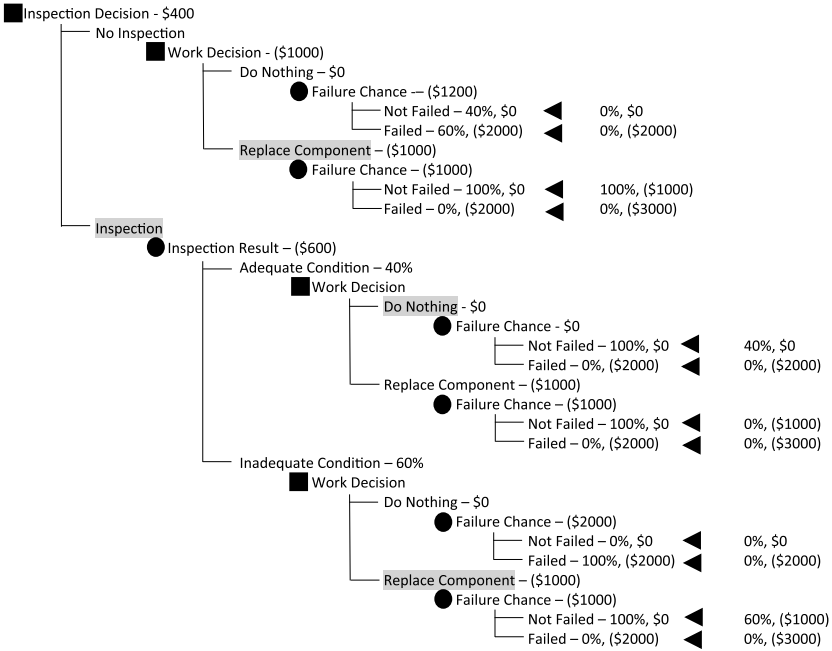
\includegraphics[width=.8\linewidth]{Grussing_VOI_Example.png}
\caption{Value of Information for Assessment Planning Example \protect\cite{grussing2018optimized}}
\label{fig:grussing_voi_example}
\end{figure}

The goal of this study is to improve the predicted probabilities (and therefore the quality of the VOI model) by analyzing historical assessment data and building a machine learning based model that accounts for previous sustainment trends. Specifically, classification models are developed to estimate the probability of a new assessment score falling into either the "Do Nothing" (Green) or "Repair" (Not Green) maintenance decision regions. In practice, this approach could be extended to include additional decision regions, such as "Replace" or "Renovate" depending on the maintenance manager's priorities. To accomplish this, an exploratory data analysis and Principal Component Analysis (PCA) are first performed to identify the most informative component parameters, followed by an evaluation and comparison of logistic regression, decision tree, and artificial neural network (ANN) models.

\subsection{Dataset}

The dataset used for this study comes from assessment data in the Sustainment Management System (SMS) BUILDER platform developed by Construction Engineering Research Laboratory (CERL) \cite{erdc_sms_roc}. Although the full dataset consists of approximately 2.7 million observations, a subset corresponding to the boilers material equipment category (MEC), consisting of 12,832 assessments, is used for detailed analysis and model development. Observations include both a manually collected direct condition rating and a predicted condition index generated from component information using the SMS Weibull degradation model at the time of an assessment. Multiple observations can be generated for given components if they have multiple assessment records. The observation's predicted Condition Index (CI) is generated using the following:

\begin{equation}
\label{eq:sms-weibull-ci}
\mathrm{CI}(t) = A \left( \frac{100}{\mathrm{CI}_{\mathrm{T}}} \right)^{ -\left(\frac{t}{\beta}\right)^{\alpha} }
\end{equation}

Where $\mathrm{t}$ is the normalized age of the component, $\mathrm{CI_T}$ is the design life of the component, A is the initial starting condition (usually 100), $\alpha$ is the scale or characteristic age of replacement, and $\beta$ is the shape or degradation parameter. The $\alpha$ and $\beta$ parameters are provided from a per specification reference catalog within the SMS, however these values can be shifted after assessments to adjust the curve to fit to the assessed condition. In cases where components have multiple assessments, the SMS $\alpha$ and $\beta$ shift calculations are applied prior to calculating the predicted CI to ensure continuity with the prediction at the time of the assessment. Additional component attributes included in each observation are detailed in Table~\ref{table:assembly}.

Assessment scores generally are collected as "Direct Condition Ratings", amounting to a selection from 9 possible score options. An example criterion for these scores can be found below in Table \ref{table:AssessmentScores} (Not all organizations have exactly the same criterion, but the score choices are always the same). Most organizations have additional guidance through large (sometimes thousands of pages) assessment guides. Within these guides, direction is provided on the types of components to inventory and assess, when and how to input comments about the assessment, additional criterion for scoring for specific component types, and other data quality governance. 

\begin{table}[htbp]
\caption{Assessment Observation Data}
\label{table:assembly}
\centering
\small
\renewcommand{\arraystretch}{1.25}
\begin{tabular}{l p{4in}}
\hline\hline
\multicolumn{1}{c}{Column (Type)} &
\multicolumn{1}{c}{Description} \\
\hline
Id (Int) & Unique identifier for the observed component.\\
Spec (Int) & Unique identifier for the specification. (Ex. 2 HP Pump, 400 gallon AST.) \\
MEC (Int) & Unique identifier for the Material Equipment Category. (Ex. Gas Boiler.) \\
System (Int) & Unique identifier for generic component classification. (Ex. HVAC Equipment) \\
DesignLife (Int) & Designed lifespan in years of the component. \\
Qty (Float) & Quantity of the component. Units defined by UOM. \\
UOM (String) & Unit of Measure of the component Qty. \\
NormalizedAge (Float) & Equal to $\text{ComponentAge} / \text{DesignLife}$. \\
EffectiveAge (Float) & The curve adjusted age of the component at the time of assessment \\
RSL (Float) & The adjusted remaining service life of the component. ($\text{DesignLife} - \text{EffectiveAge}$) \\
Recency (Int) & Years since the last assessment. Null for first assessments. \\
PredictedCI (Float) & Predicted Condition Index at the time of the observation. Derived from SMS Weibull Model. \\
Score (Float) & Assessor's assigned condition rating. \\
CRV (Int) & Component Replacement Value (U.S. Dollars) \\
Year (Int) & Calendar year of the assessment. \\
Month (Int) & Calendar month of the assessment. \\
Climate (Int) & Department of Energy (DOE) based climate zone code \cite{doe_building_america_climate_guidance}. \\
Fac (Int) & Unique identifier for the type/purpose of the component's parent asset. \\
AssetAge (Int) & Age in years of the component's parent asset. \\
AssetDesignLife (Int) & Designed lifespan in years of the component's parent asset. \\
PrevScore (Float) & Previous assessment score. Null for first assessments. \\
\hline
\multicolumn{2}{l}{$\ast$ System->MEC->Spec form a data hierarchy similar to a WBS like classification structure.} \\
\multicolumn{2}{l}{$\ast$ Data has been obfuscated, replacing readable definitions with numbers.} \\
\hline\hline
\end{tabular}
\normalsize
\end{table}

\begin{table}[htbp]
\caption{Example Assessment Scoring Criteria based on USACE Guidance.}
\label{table:AssessmentScores}
\centering
\small
\renewcommand{\arraystretch}{1.25}
\begin{tabular}{l r p{3.5in}}
\hline\hline
\multicolumn{1}{c}{Rating} &
\multicolumn{1}{c}{CI Value} &
\multicolumn{1}{c}{Rating Definition} \\
\hline
Green (+) & 100 & Entire component is free of observable distresses. Like-new condition. \\
Green & 95 & No serviceability or reliability reduction. Slight degradation but noncritical. No work other than routine maintenance is required. \\
Green ($-$) & 88 & Slight or no serviceability or reliability reduction. Some noticeable degradation is present but remains noncritical. No work other than routine maintenance is required. \\
Amber (+) & 79 & Serviceability or reliability is degraded but remains adequate. Moderate deterioration is present but remains noncritical. Minor repairs are needed. \\
Amber & 68 & Serviceability or reliability is noticeably impaired. Moderate deterioration or damage requires corrective repairs. \\
Amber ($-$) & 60 & Significant serviceability or reliability loss. Significant degradation or damage requires major rehabilitation or overhaul. \\
Red (+) & 50 & Significant serviceability or reliability loss. Repairs are not feasible, and replacement is needed. \\
Red & 25 & Severe serviceability or reliability reduction may result in loss of use or safety. Immediate replacement is warranted. \\
Red ($-$) & 10 & Complete degradation and loss of serviceability. May result in damage to surrounding components. Replace immediately. \\
\hline\hline
\end{tabular}
\normalsize
\end{table}

\FloatBarrier

\section{Exploratory Data Analysis}

As a first step of exploratory analysis, the shapes of individual columns of the dataset were visualized to understand the distributions of the data. Although distributions were produced and explored for all fields in the dataset, only the distributions most relevant to the motivating questions are highlighted in this report. For the purposes of this project, three of the most pertinent columns in the dataset include the predicted condition score, or CI, of the Weibull degradation model, the actual observed score of the assessor (i.e., assessor rating), and Remaining Service Life (RSL). Because RSL is calculated from the component's design life and curve adjusted effective age, it is directly tied to the Weibull degradation curve used to generate the predicted CI and provides an intuitive measure of remaining component life (Figure \ref{fig:rsl_dist}). Based on the histograms for the condition variables, there is a visually identifiable difference between the expected degradation and the assessed scores (Figures \ref{fig:ci_dist} and \ref{fig:score_dist}). There is also a heavy observable bias toward ratings of 88 in the assessed boiler condition scores compared to the Weibull predicted CIs.

\begin{figure}
\centering
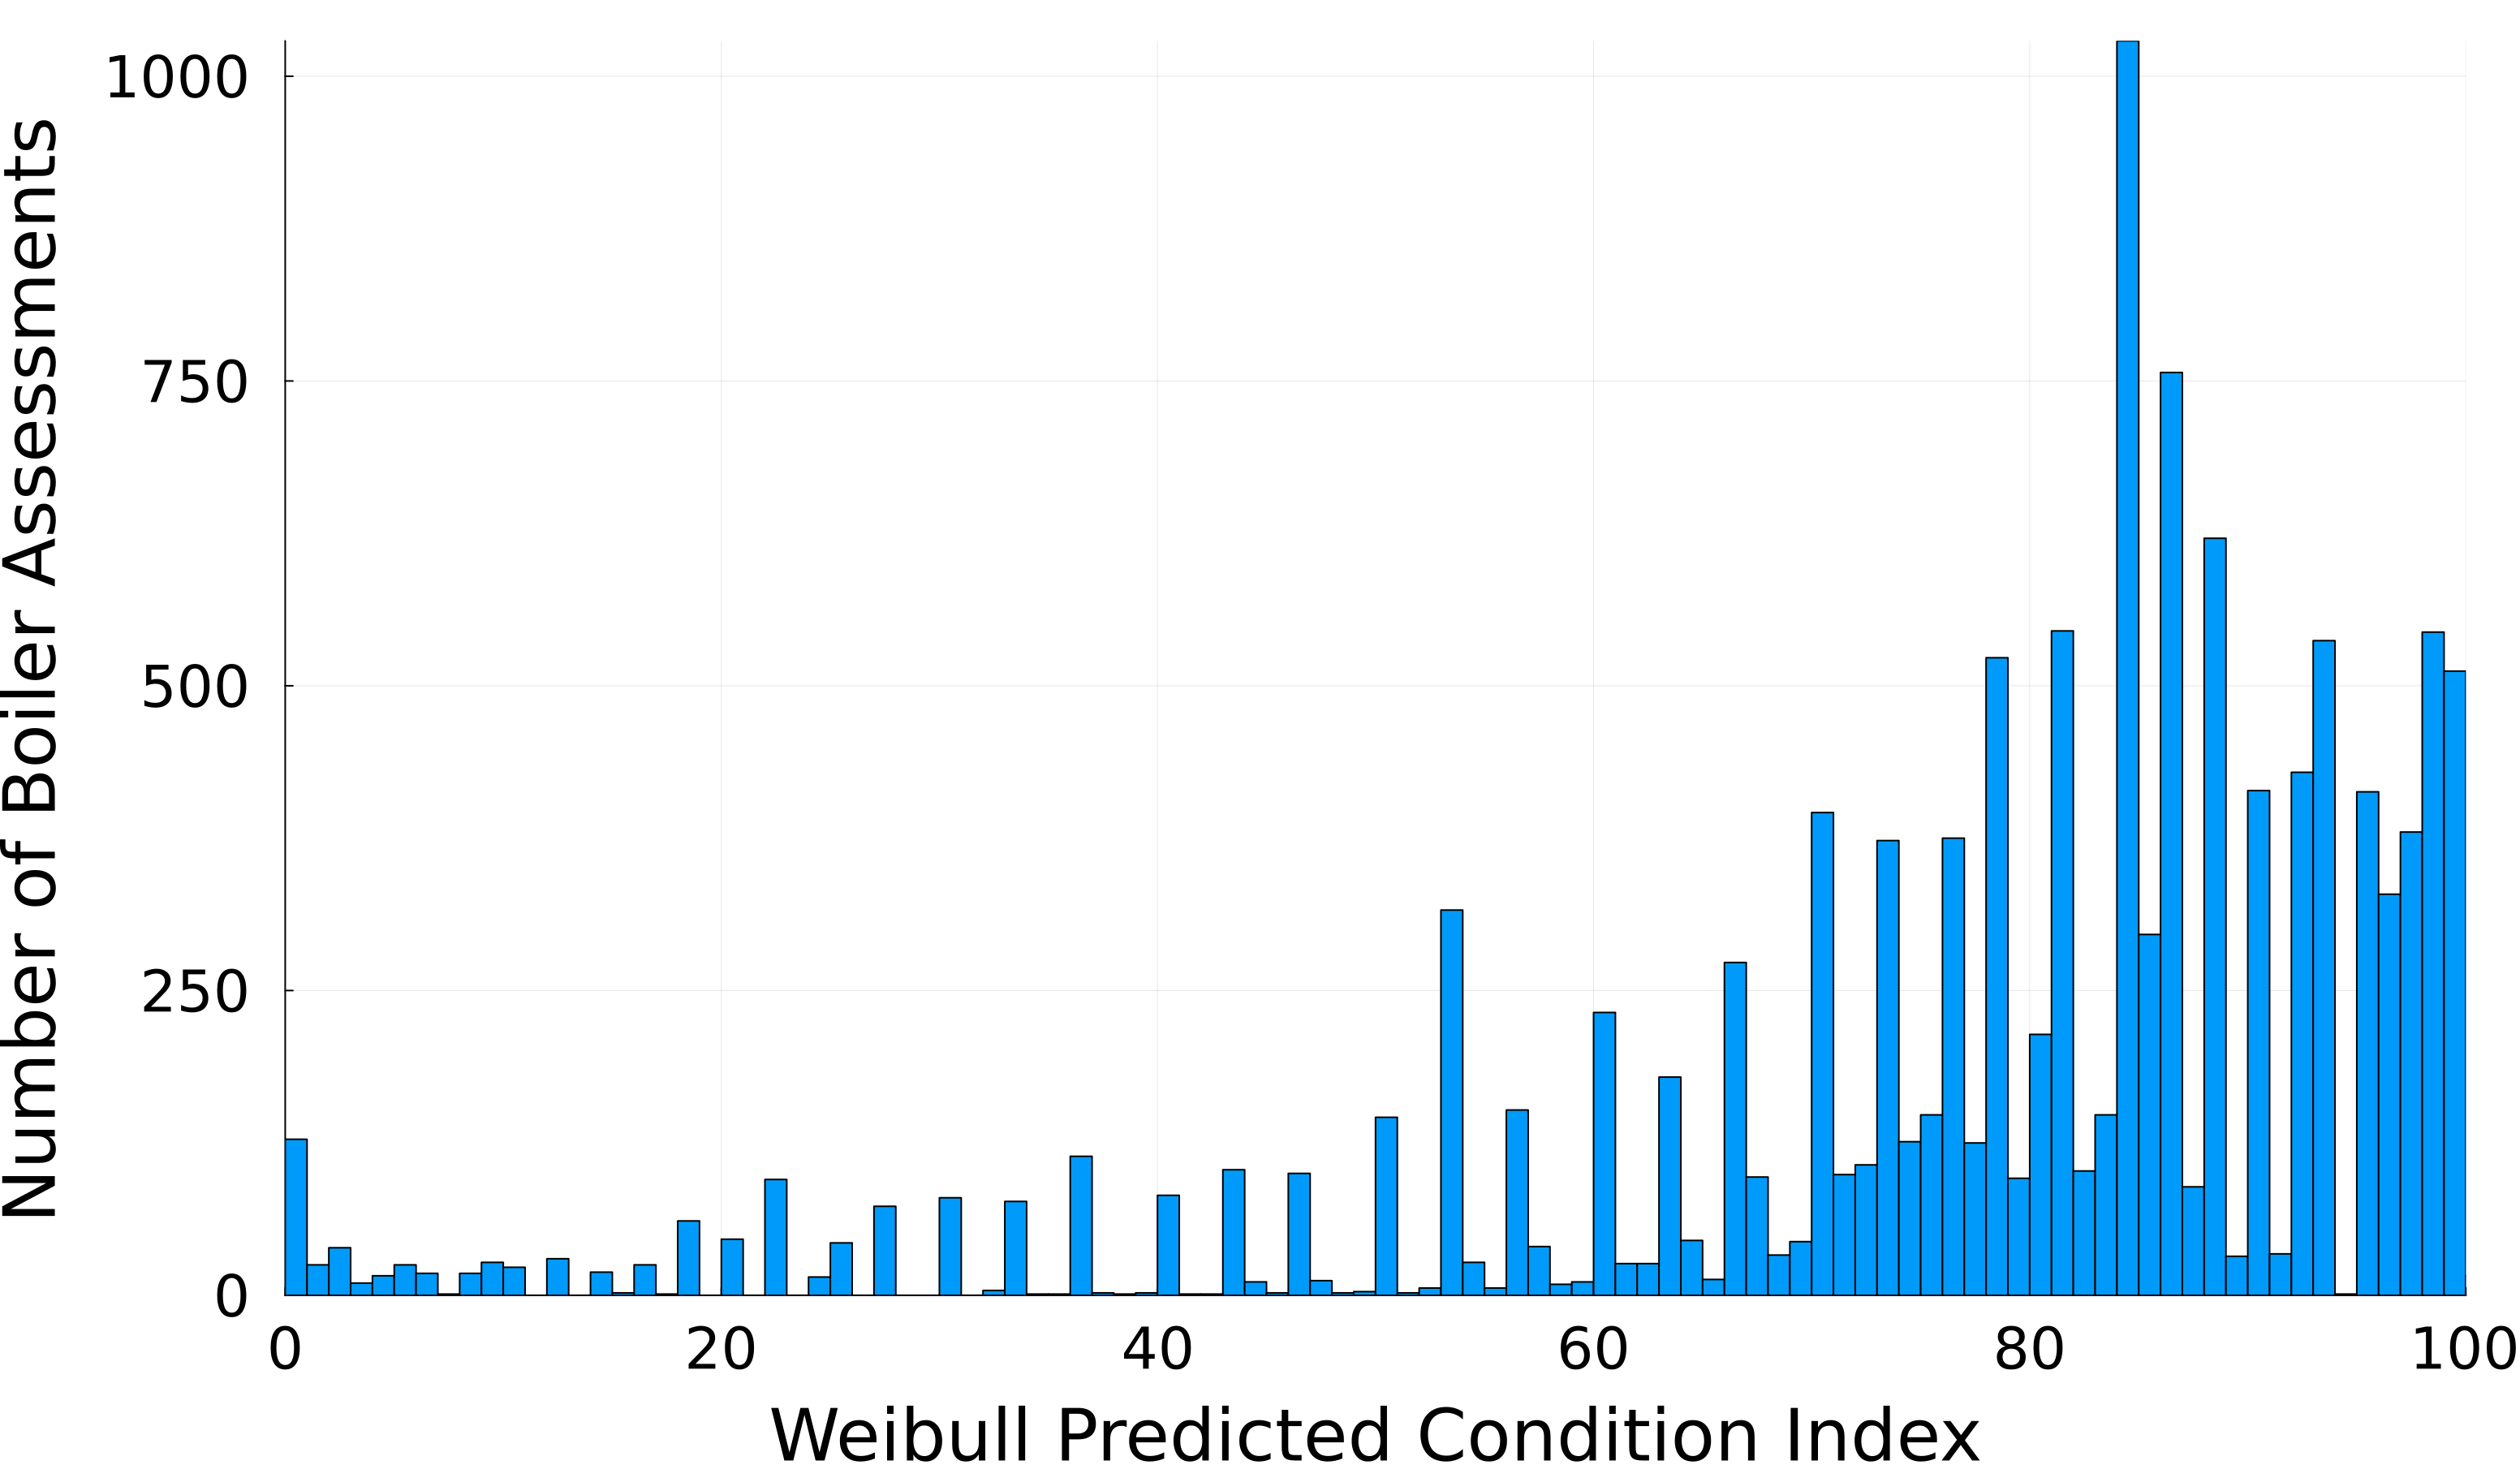
\includegraphics[width=.8\linewidth]{ci_dist.png}
\caption{Predicted CI Distribution}
\label{fig:ci_dist}
\end{figure}

\begin{figure}
\centering
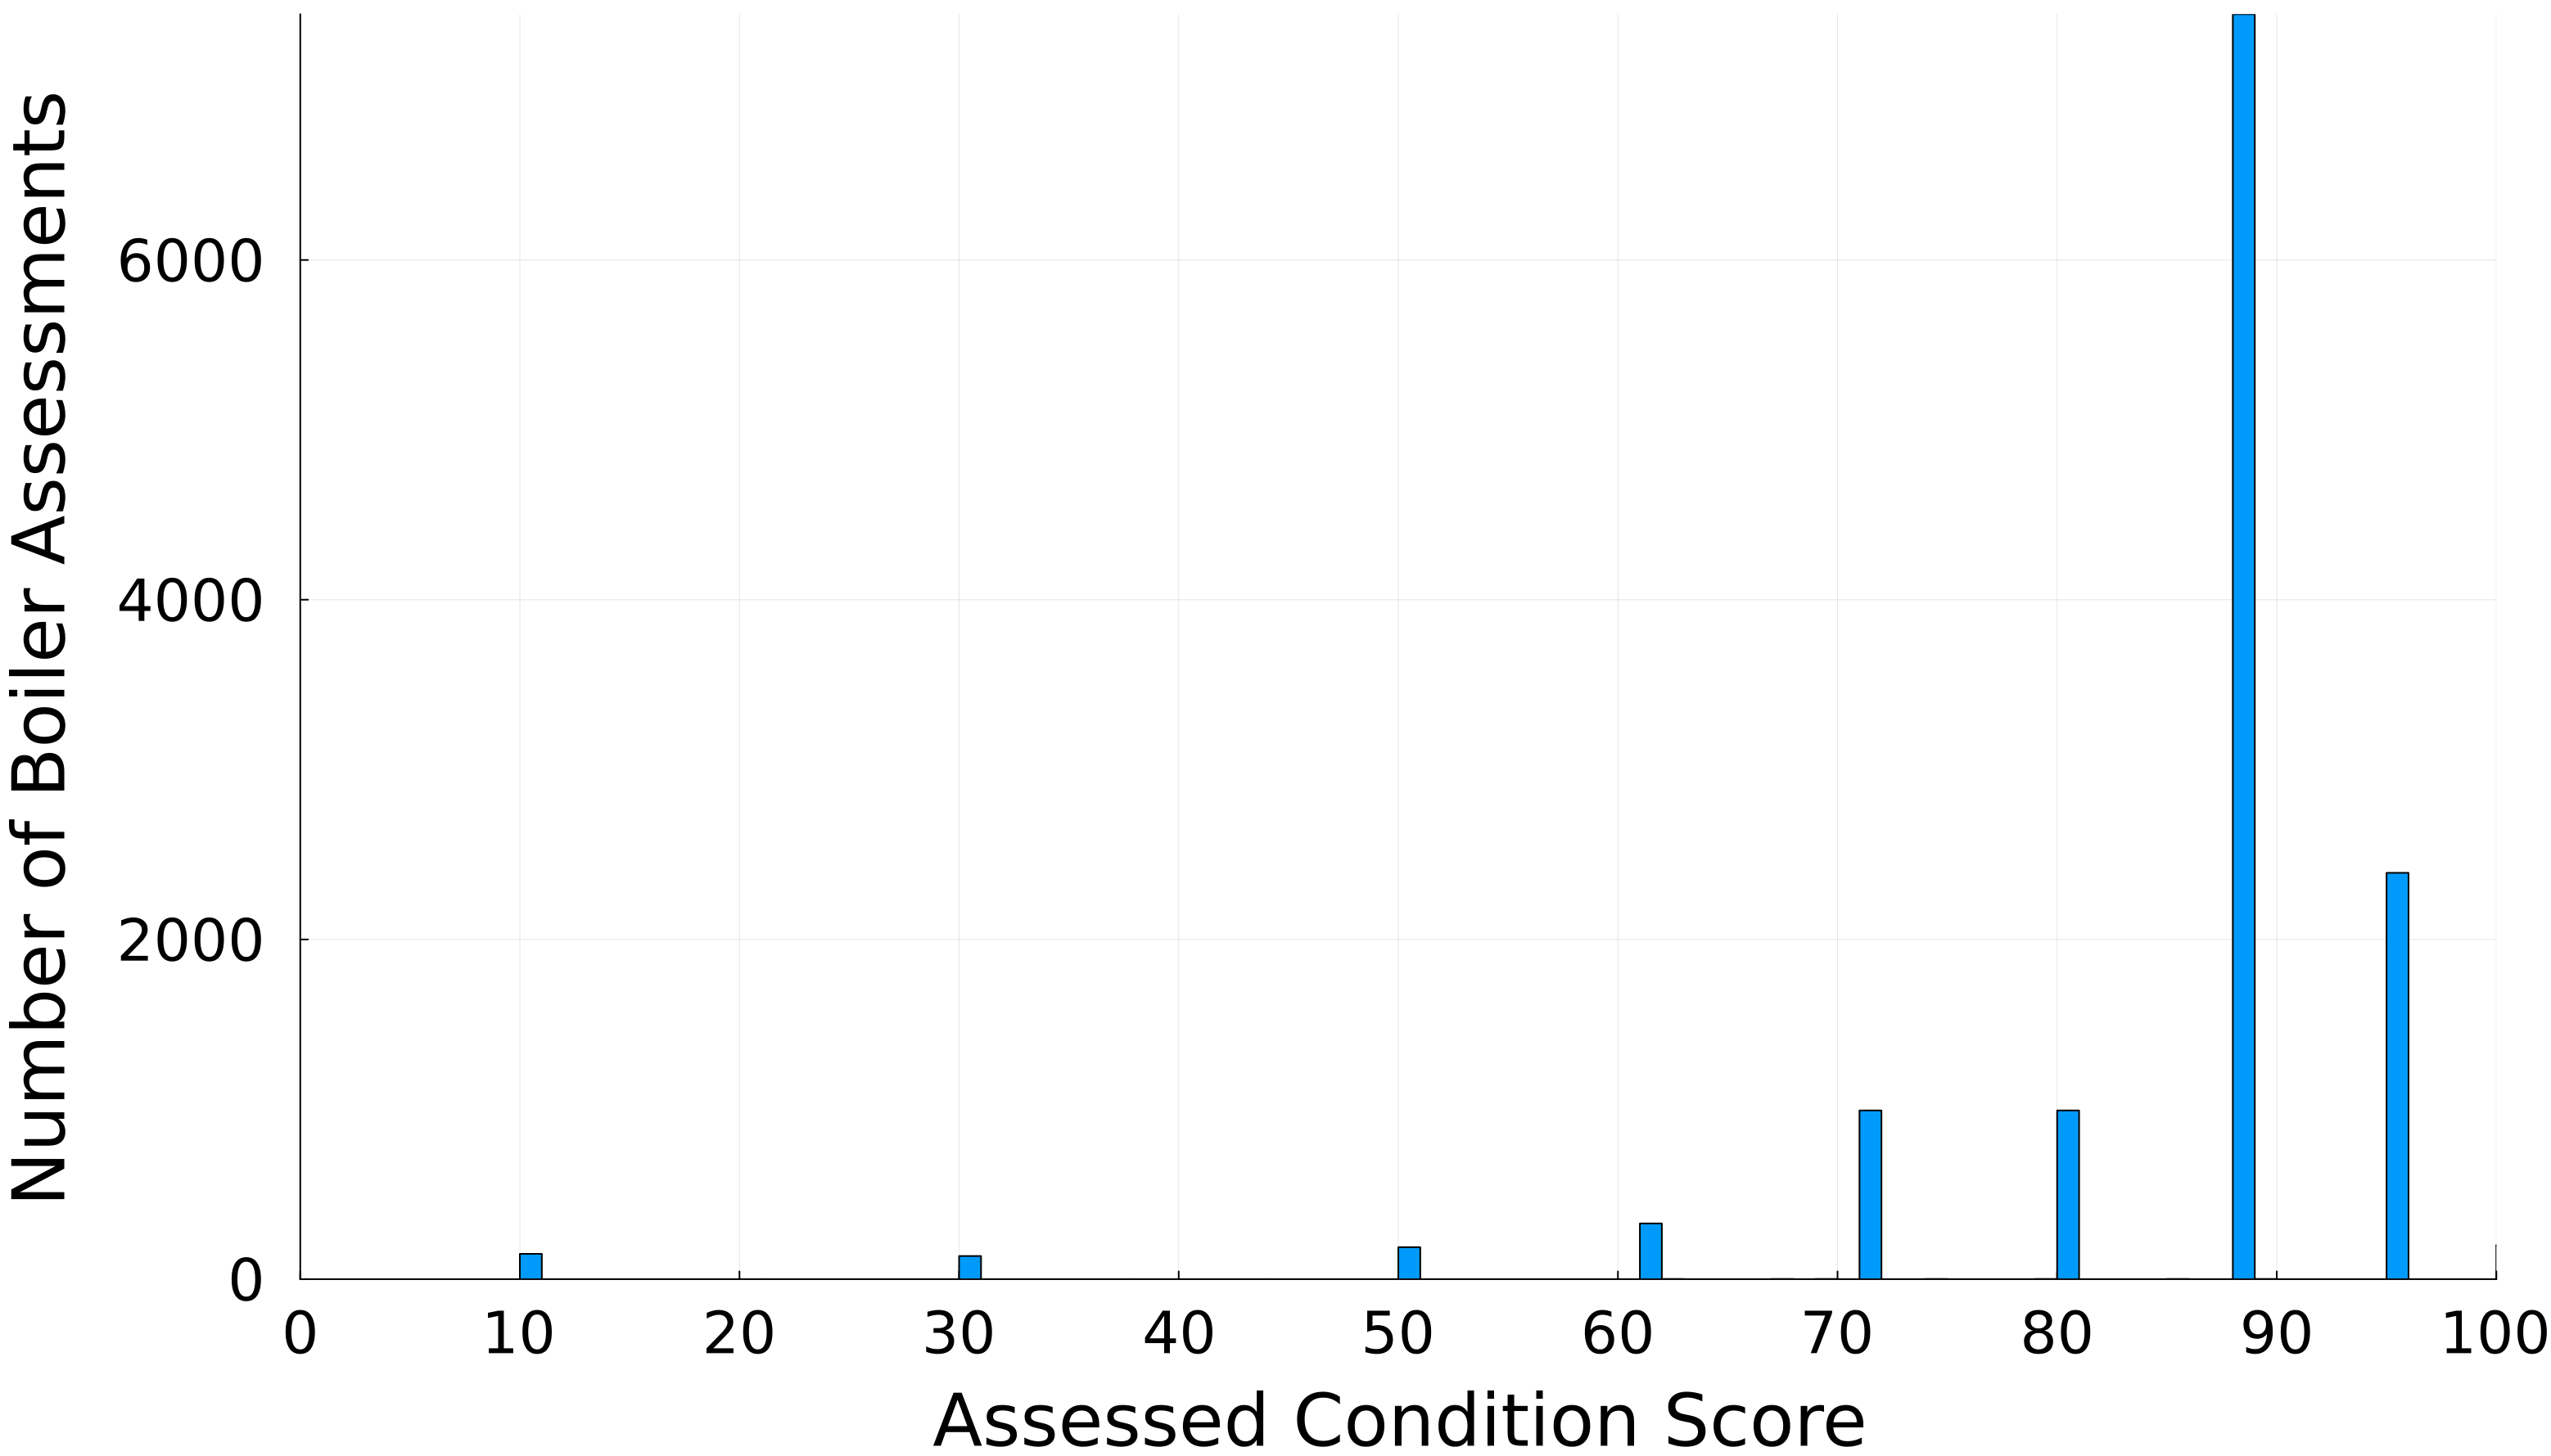
\includegraphics[width=.8\linewidth]{score_dist.png}
\caption{Assessment Score Distribution}
\label{fig:score_dist}
\end{figure}

\begin{figure}
\centering
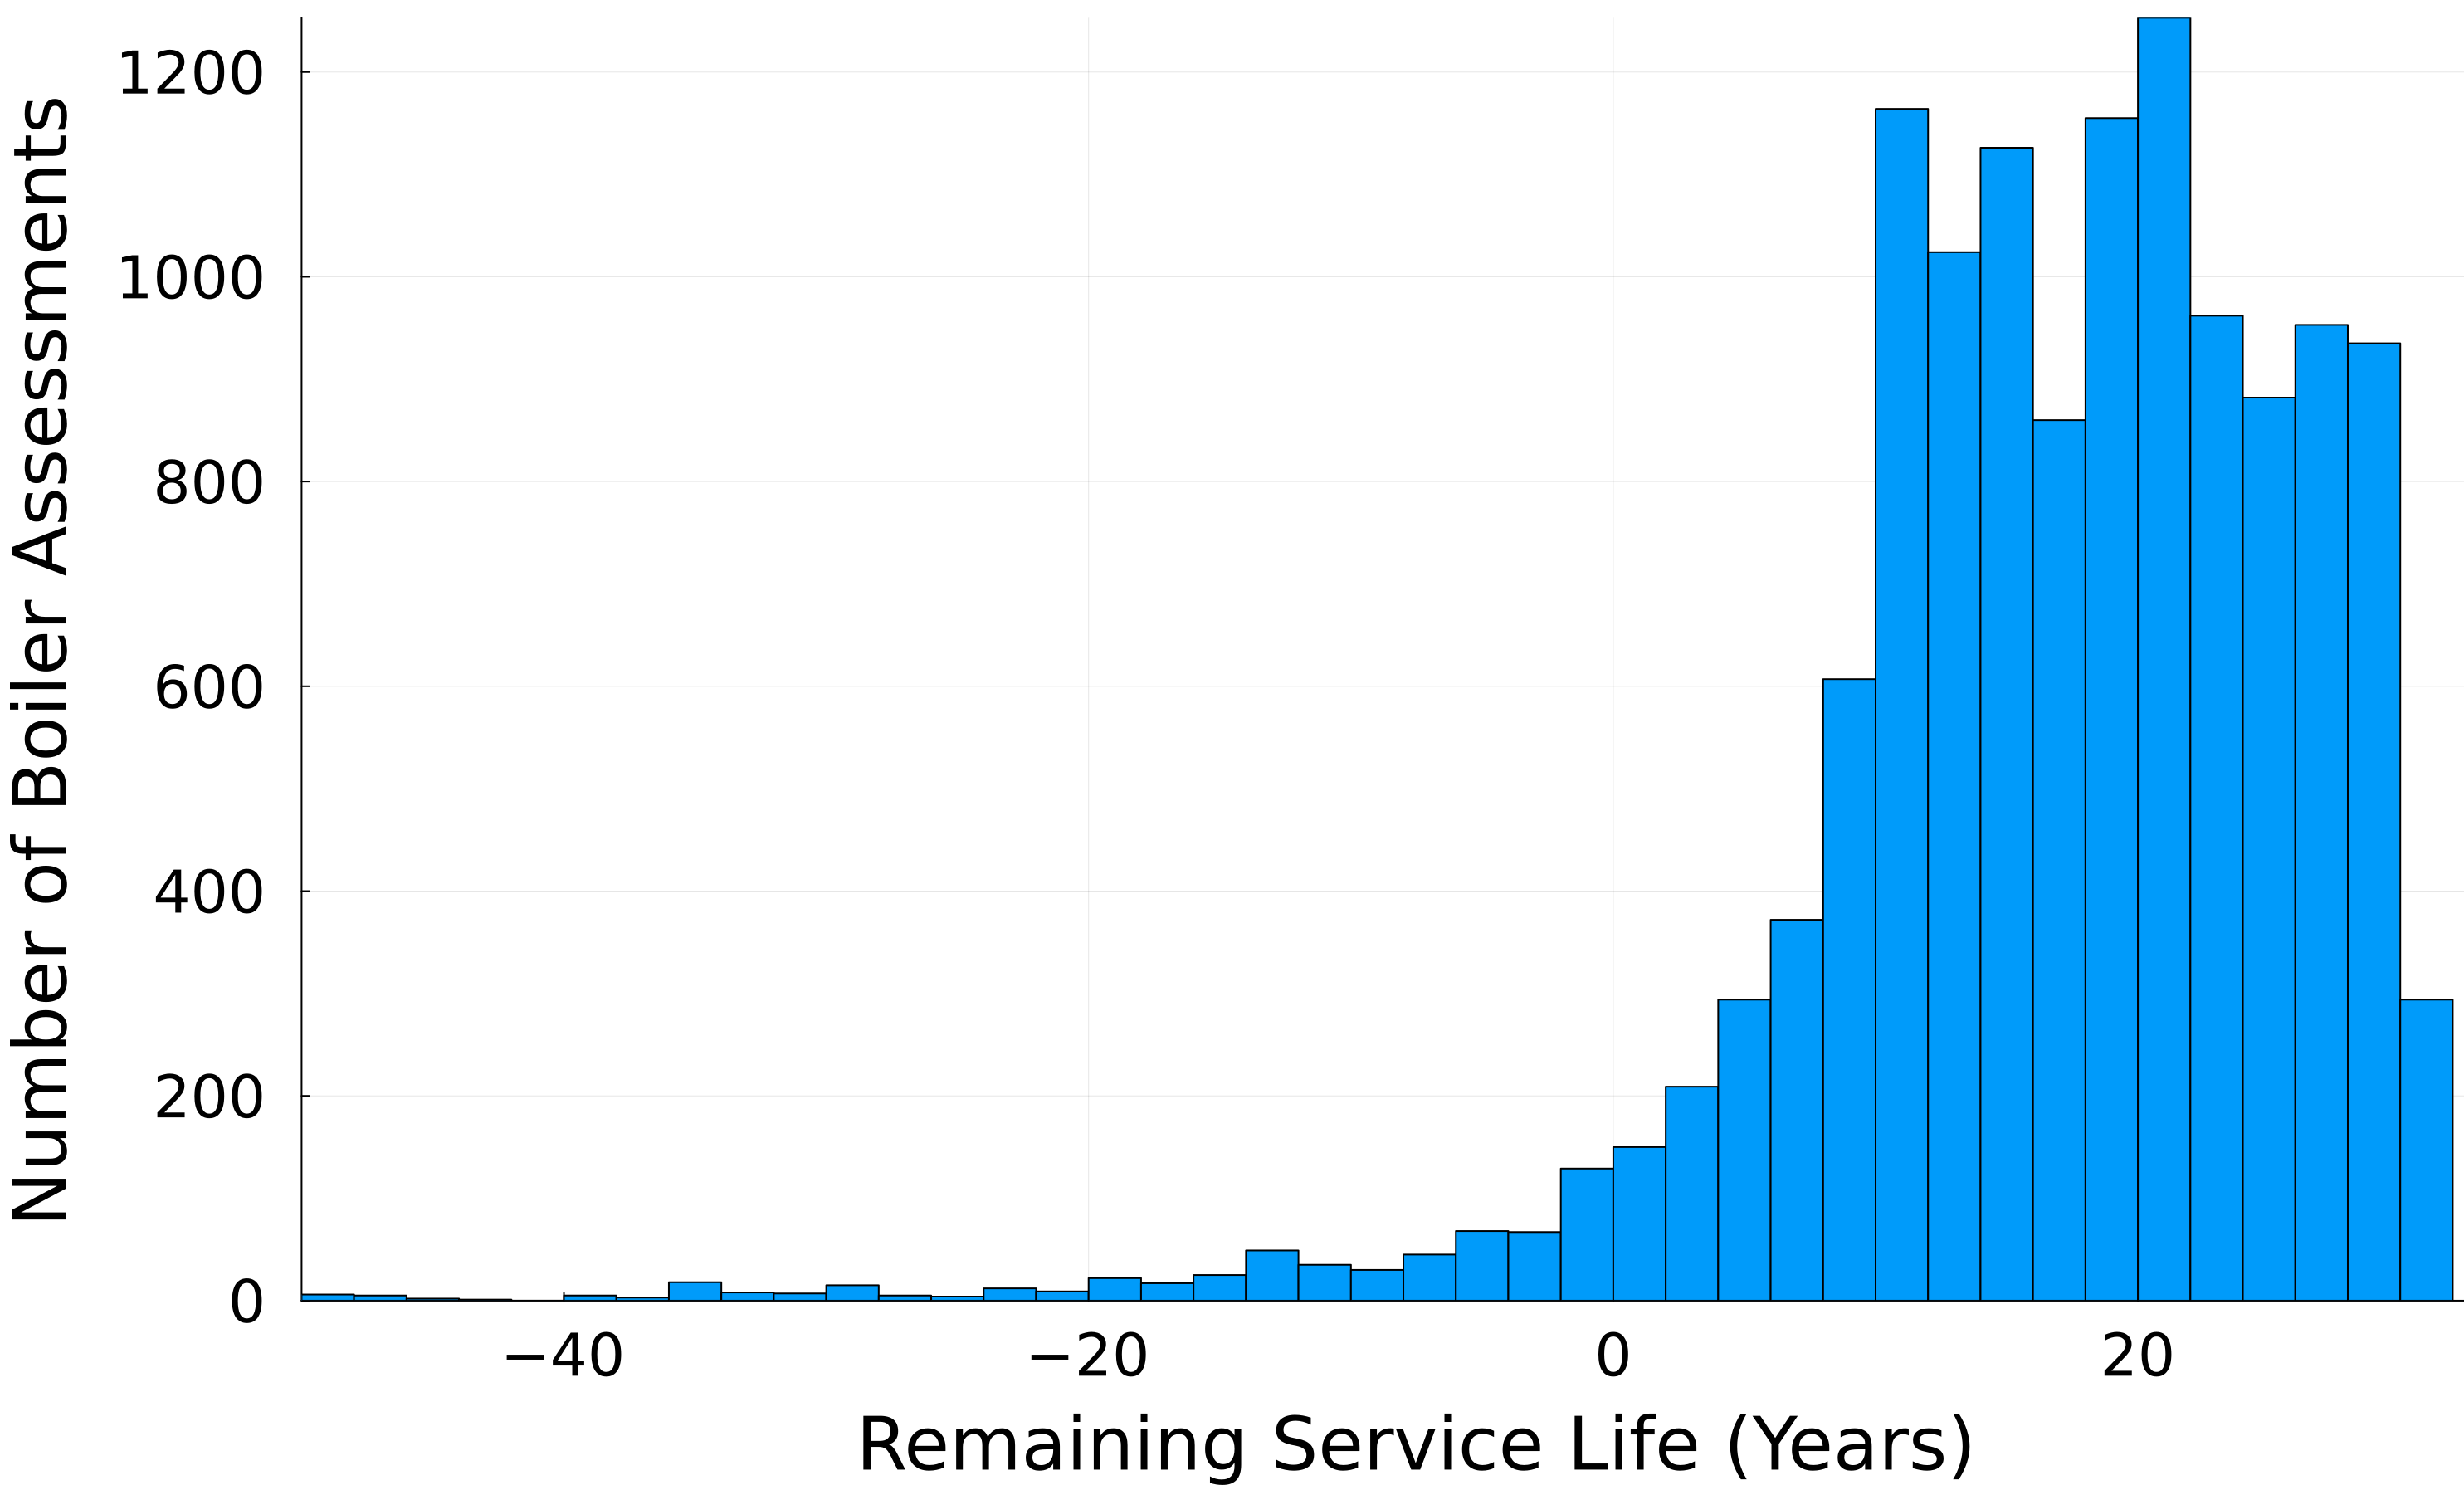
\includegraphics[width=.8\linewidth]{rsl_dist.png}
\caption{Remaining Service Life Distribution}
\label{fig:rsl_dist}
\end{figure}

There are some rational narratives that can explain the disagreement in predicted and assessed scores.  The SMS system from which the observations are sourced is used by organizations to plan maintenance management.  Work analysis rules are put into place within the system to prioritize maintenance funding allocation.  For HVAC systems, a typical ruleset will specify that components with a CI less than 85 should be marked for repair action, and components with an RSL of less than 2 should be marked for replacement \cite{rsmeans_uniformatii}. If maintenance dollars are being executed by that guidance, then it would be expected that assessors rarely come across boilers with condition less than 85.  This also makes rational sense from a facility function perspective, heating, ventilation, and air conditioning (HVAC) systems tend to get immediate attention when they fail, as they are considered critical for most facilities. Additionally, this bias is not unique to SMS data, and has been observed in other inspection and assessment-based condition datasets. One such example is an Ontario bridge inspection dataset where a similar condition clustering is observed around a score of 77 (based on that unique condition rating system) \cite{ontario_bridge_conditions_2021}.

Additionally, based on this visual inspection of the assessed score distribution, questions were formulated to attempt to identify how data could be classified to distinguish between boilers that are kept to specified condition versus those that are allowed to deteriorate. Answers to these questions may assist in feature selection for the construction of a prediction model. Looking at several of the other distributions, including Month (Figure \ref{fig:month_dist}) and Climate (Figure \ref{fig:climate_dist}), raised possible considerations. Specifically, the following questions were considered: (1) Does RSL (or other lifecycle variables) correlate with assessor ratings?; (2) Does the month (i.e Season) of the assessment impact the expected assessed condition for boilers?; (3) Does the climate (warm or cold) impact expected assessed condition?; and finally, (4) What other ways could the data be classified to help with prediction models?

\begin{figure}
\centering
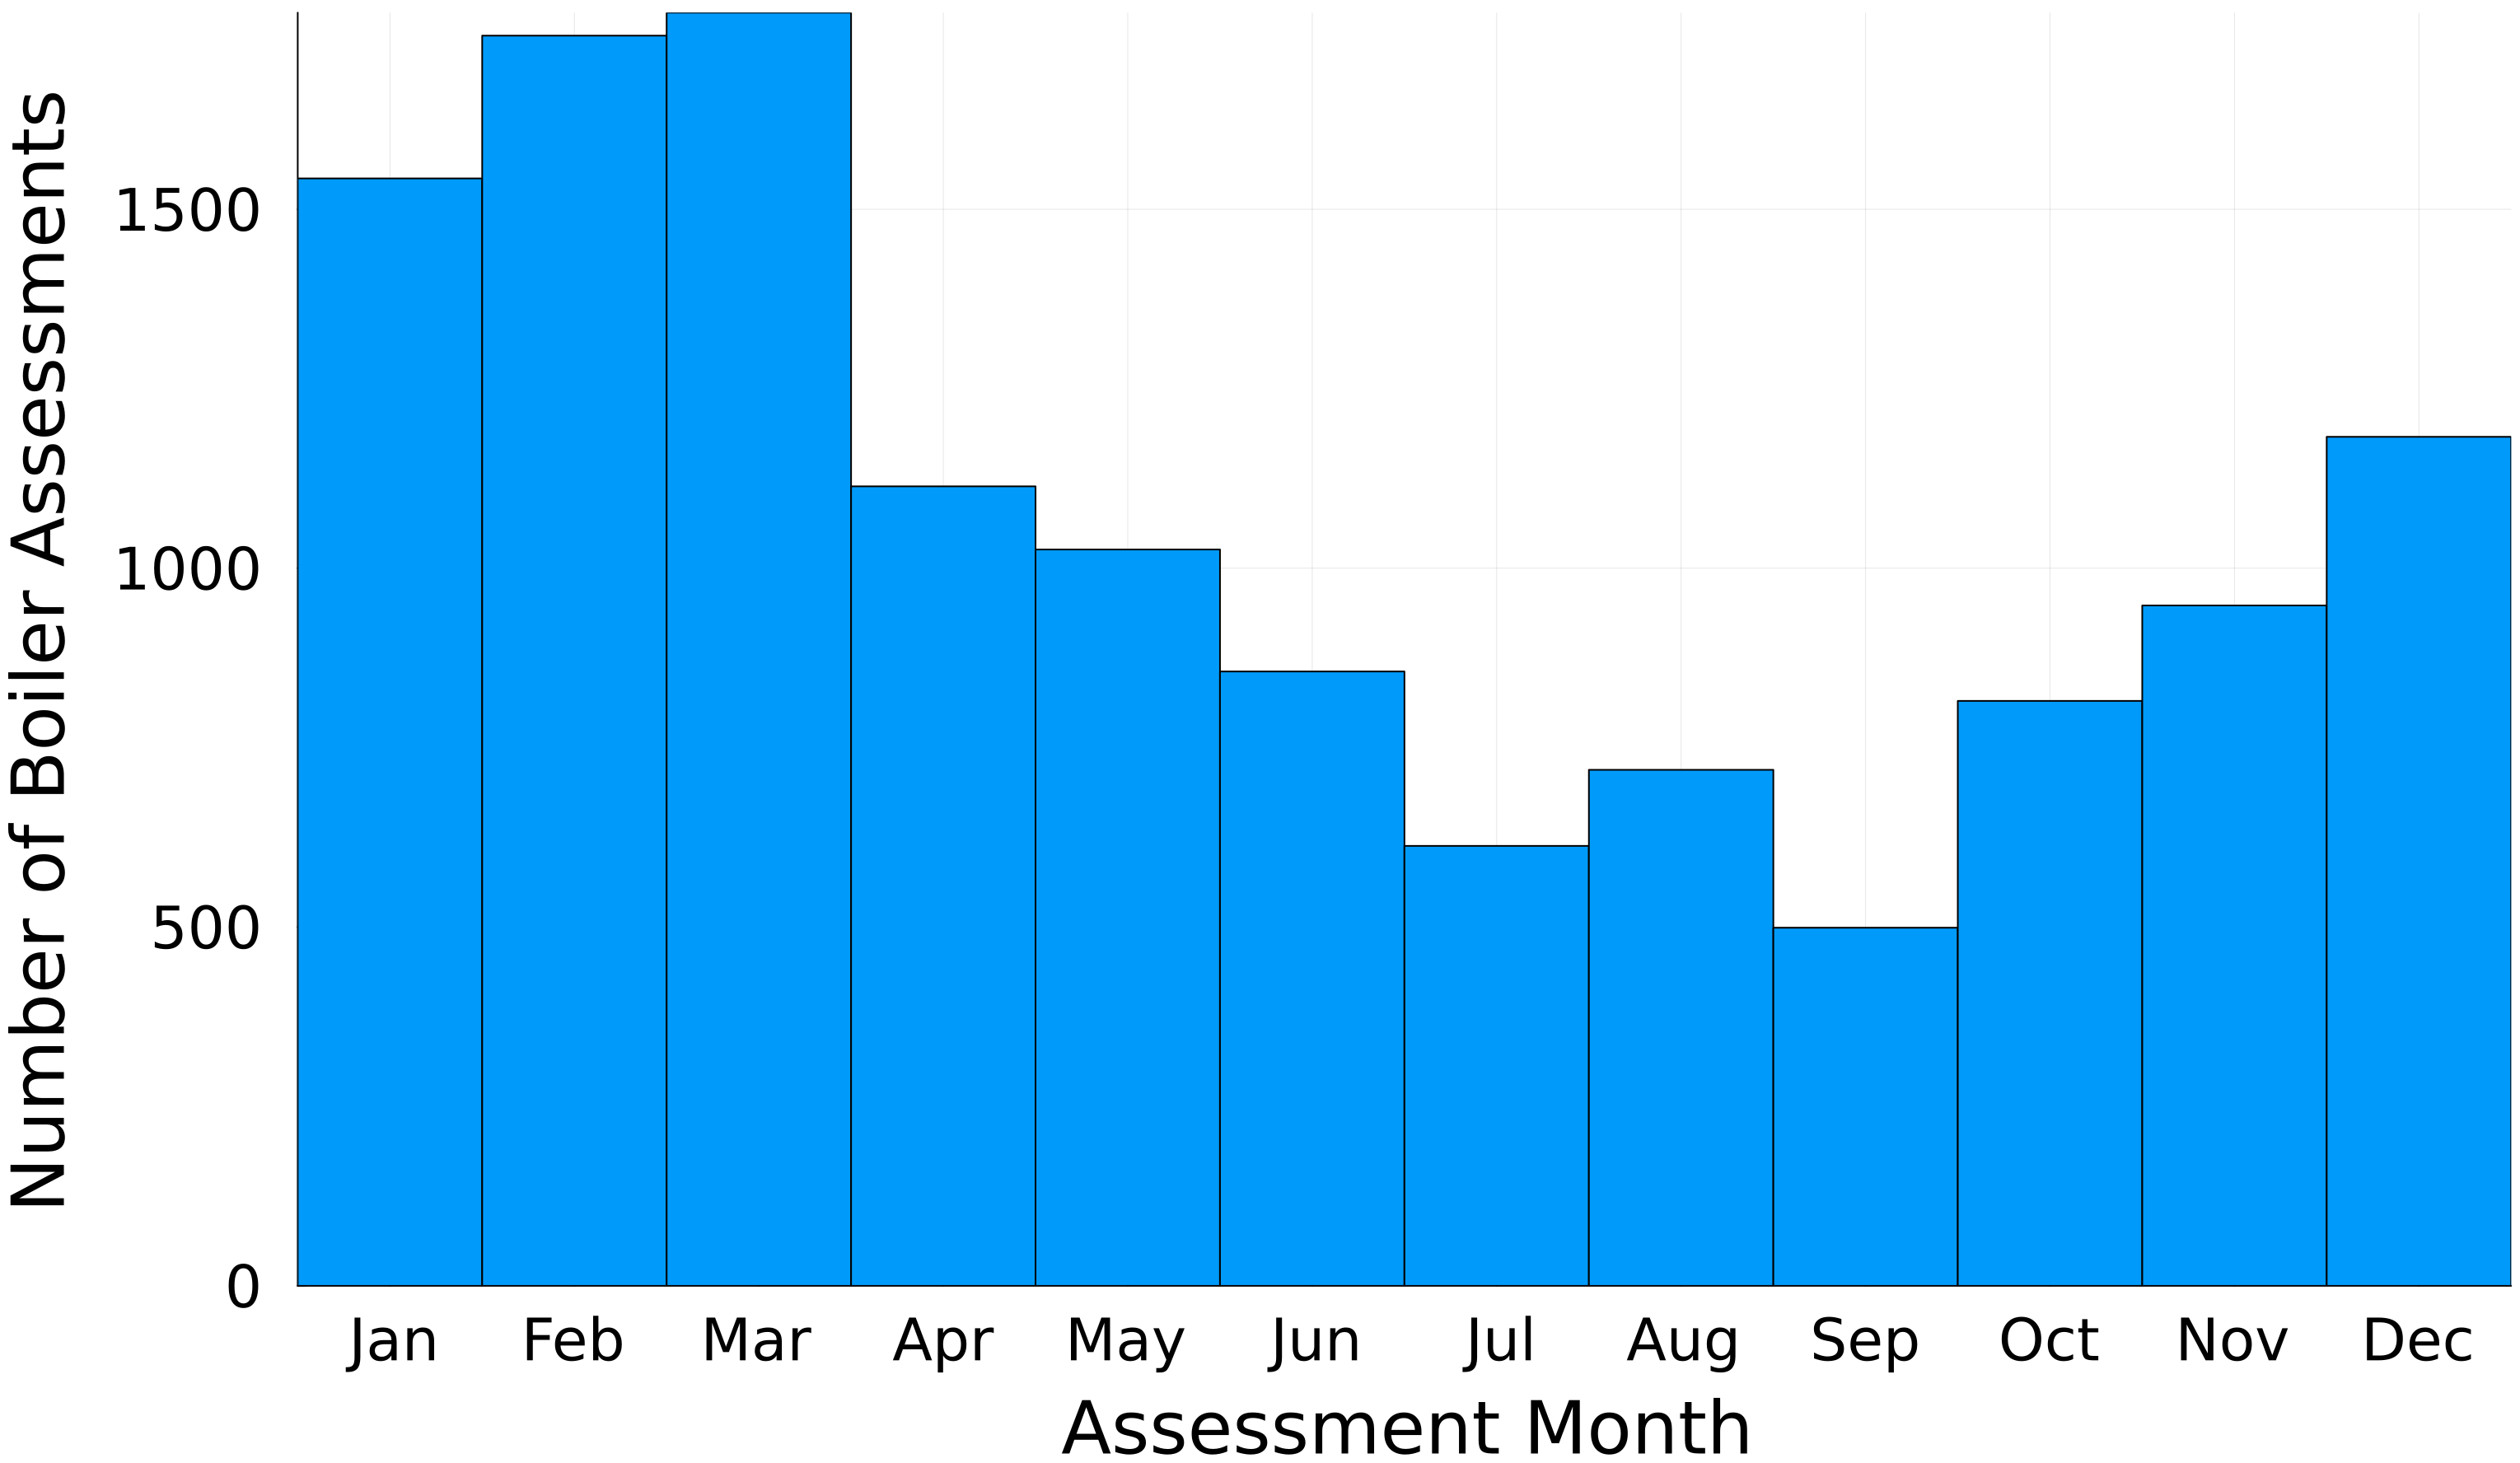
\includegraphics[width=.8\linewidth]{month_dist.png}
\caption{Assessment Month Distribution}
\label{fig:month_dist}
\end{figure}

\begin{figure}
\centering
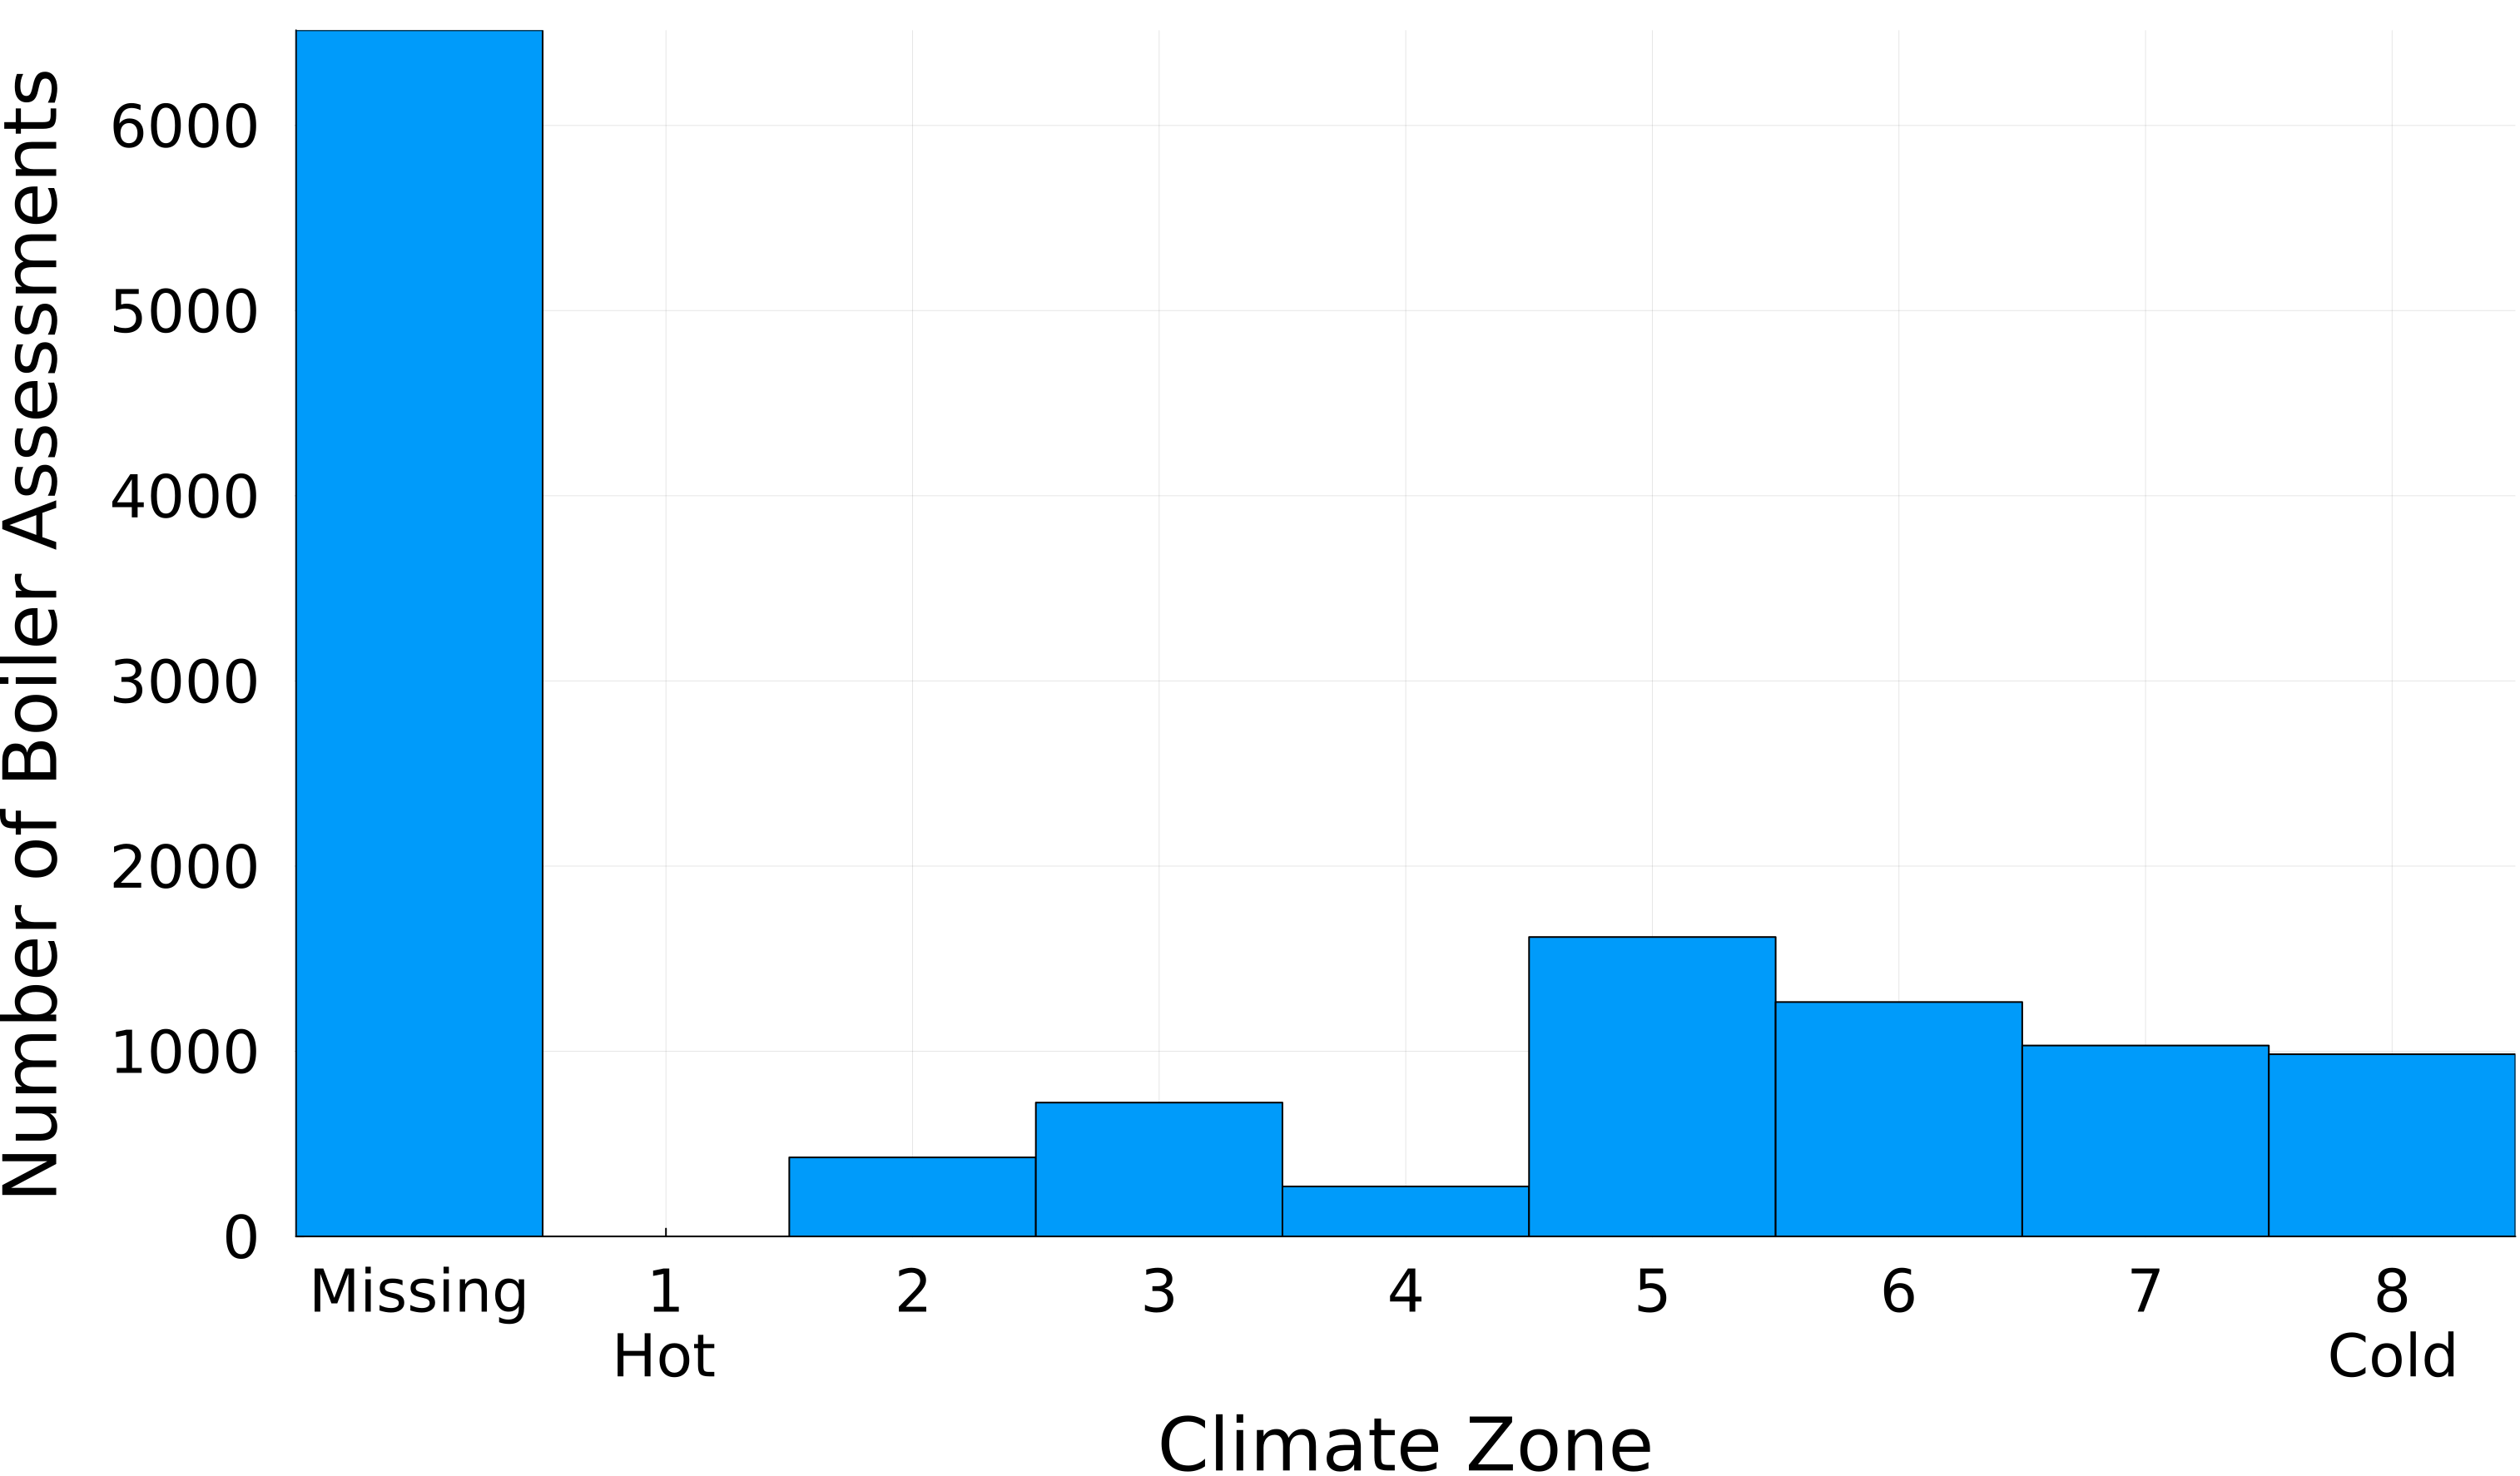
\includegraphics[width=.8\linewidth]{climate_dist.png}
\caption{Assessment Climate Distribution}
\label{fig:climate_dist}
\end{figure}

\FloatBarrier

\subsection{Pairwise Correlation Analysis}

A pairwise correlation analysis was completed to understand relationships among the features in the raw dataset. To this end, Spearman's rank correlation coefficient ($\rho$), which is a nonparametric measure of the strength and direction of the monotonic relationship between two variables \cite{scipy_spearmanr,uva_correlation}, was calculated for each combination of pairs among the following set of fifteen features: NormalizedAge, EffectiveAge, RSL, Recency, PrevScore, PrevAssessed, PredictedCI, Score, Qty, AssetAge, AssetDesignLife, LogCRV, Month, Year, and Climate. Statistical significance of the correlation between variable pairs was also calculated. The results of this analysis are visualized in Figure \ref{fig:spearman_heatmap} as a heatmap of correlation coefficients. Positive correlation coefficients, shown as red squares in the heatmap, indicate a positive monotonic relationship, while negative correlation coefficients, shown as blue squares in the heatmap, represent a negative monotonic relationship.

In Figure \ref{fig:spearman_heatmap}, the strongest pairwise correlations are observed between PredictedCI and NormalizedAge, EffectiveAge, and RSL, as well as between RSL and NormalizedAge. The calculated coefficients for these relationships were -0.88, -0.81, 0.91, and -0.90, respectively, all with statistical significance at p < 0.001. However, these relationships are expected based on the characteristics of the dataset. For example, NormalizedAge is an input to the equation used to calculate PredictedCI, and EffectiveAge is used to calculate RSL. These correlations among dependent variables will need to be mitigated during the development of predictive models in order to prevent confounding.

In contrast, the relative strength of pairwise correlations with the Score variable, which represents an assessor's assigned condition rating of a given boiler, is lower. For example, the correlation coefficients with the largest magnitude are those with RSL, NormalizedAge, and PredictedCI, but their values are only 0.54, -0.53, and 0.50, respectively, each with statistical significance at p < 0.001. These results indicate that Score cannot be predicted by a single correlation with another variable, and that a multivariate approach is needed to understand the complex relationships influencing Score.

\begin{figure}
\centering
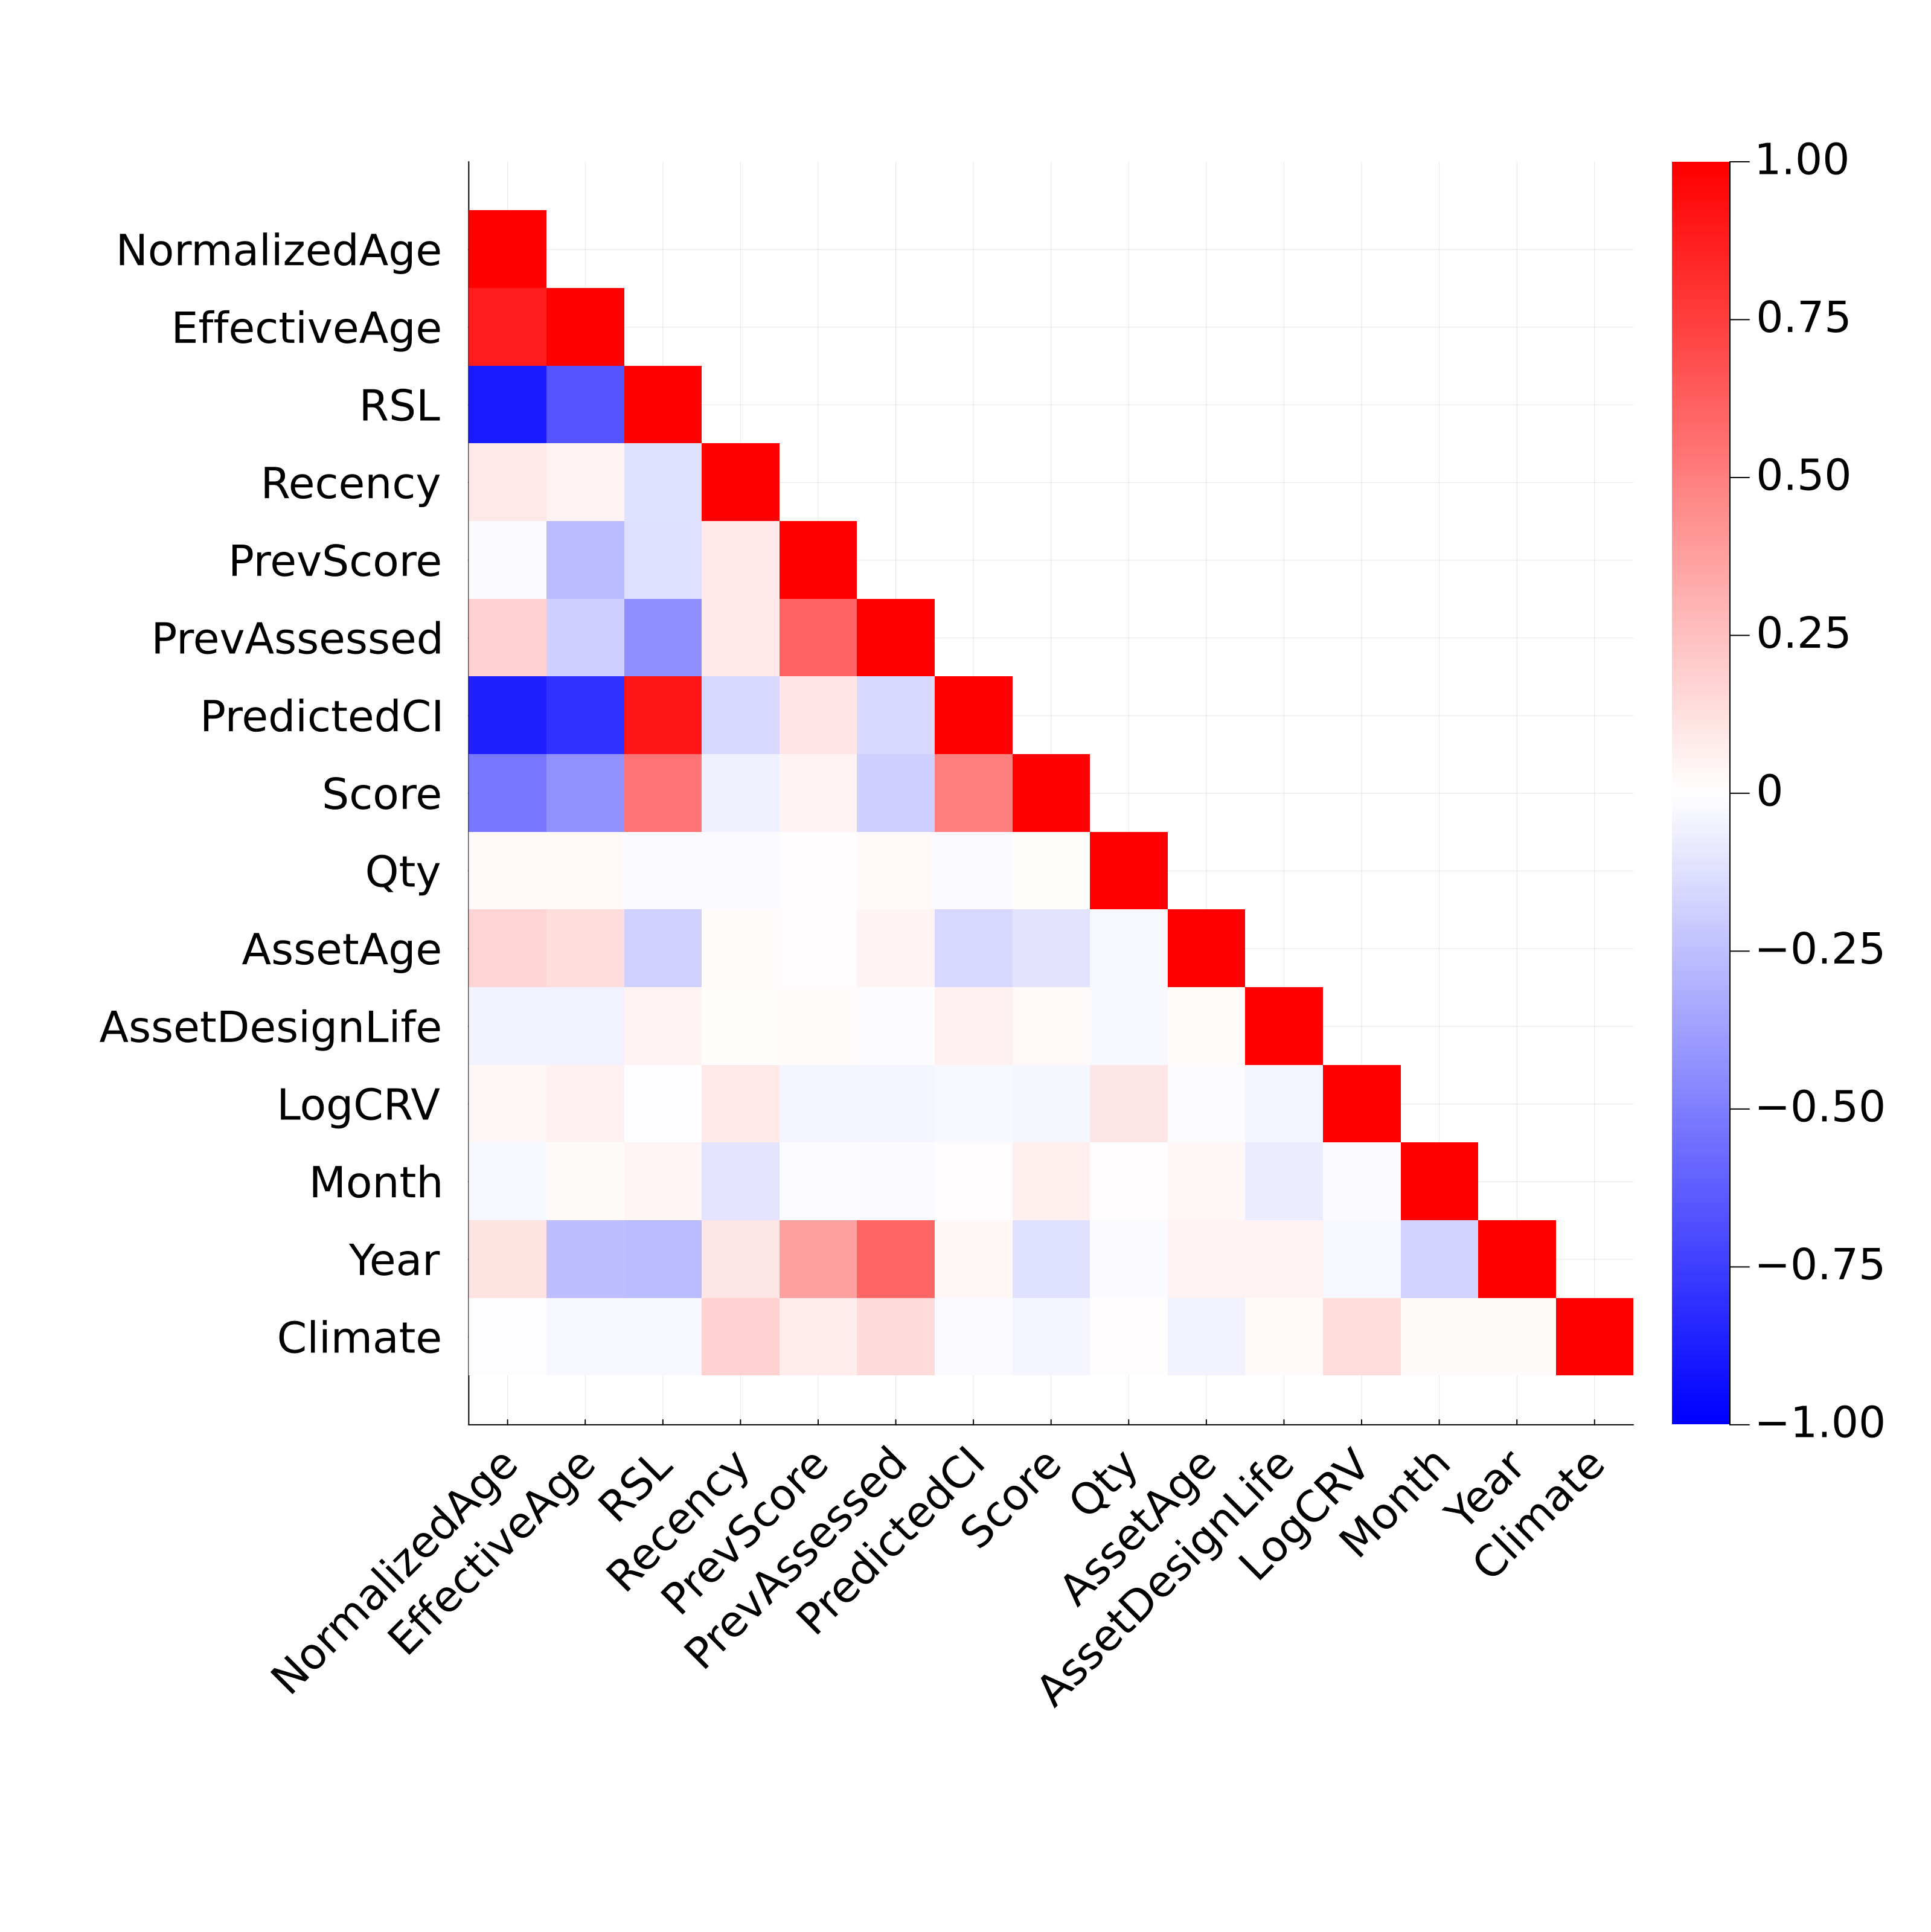
\includegraphics[width=.8\linewidth]{spearman_heatmap.png}
\caption{Spearman's rank correlation coefficients among variable pairs in the boiler dataset.}
\label{fig:spearman_heatmap}
\end{figure}

\FloatBarrier

\subsection{Additional Data Insights}

In the following analyses, green ($\mathrm{Score}\geq 88$) and not-green ($\mathrm{Score}<88$) assessment records are compared in terms of lifecycle characteristics, asset age, climate, and season of assessment. Observations may include repeated assessments of the same component.

\subsubsection{Lifecycle Characteristics and Assessment History}

Two perspectives on the relationship between asset history and current condition are provided by RSL and previous assessment scores (Figure~\ref{fig:julian_plot1}). A substantially higher average RSL (18.61) is observed for green assessments than for not-green assessments (8.76), while their average previous scores are 88.56 and 79.39, respectively. Based on the differences between these distributions, useful information for predicting assessment scores may be contained in both lifecycle characteristics and previous condition. Although the distributions overlap, further consideration of these variables in predictive modeling is supported by the general separation between the groups.

\begin{figure}[htbp]
\centering
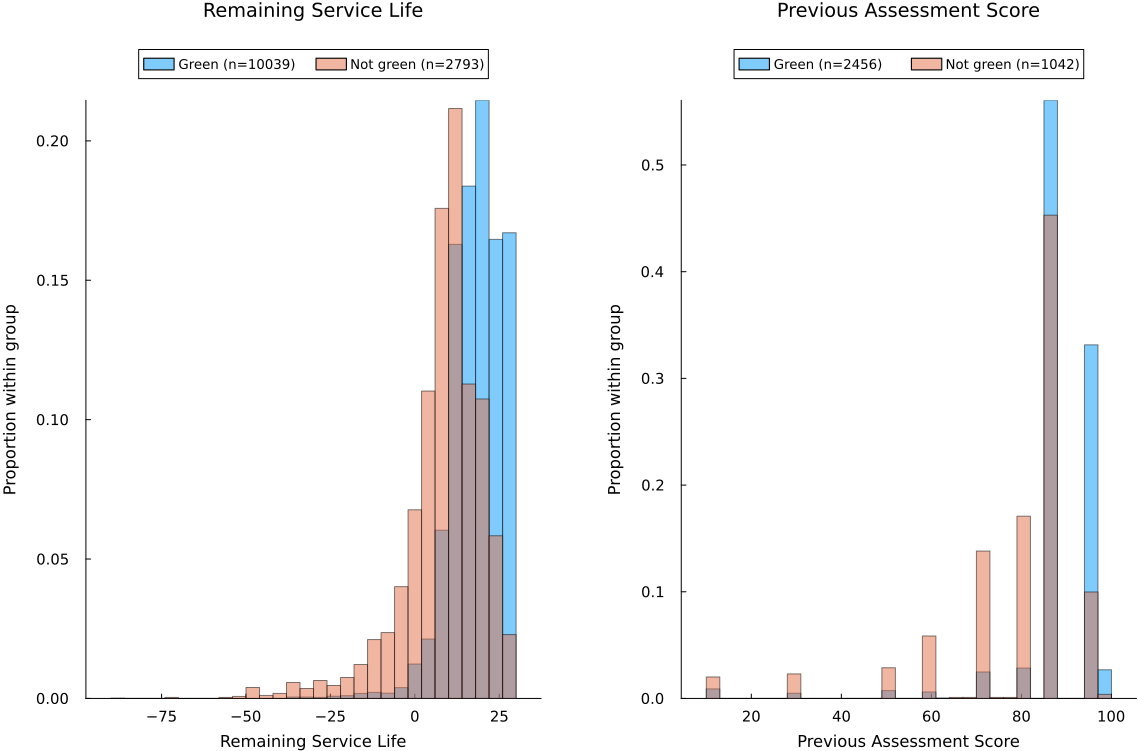
\includegraphics[width=0.95\linewidth]{interesting_plot1.png}
\caption{Remaining Service Life Distribution / Previous Assessment Score Distribution.}
\label{fig:julian_plot1}
\end{figure}

\subsubsection{Condition Status Across Asset-Age Groups}

Asset age is another important characteristic when examining differences in component condition (Figure~\ref{fig:julian_plot2}). The proportion of not-green assessments generally increases with age, rising from approximately 10.9\% for assets younger than 10 to 30.3\% for those between 30 and 40, before decreasing to 24.1\% for assets aged 40 or older. Although the relationship is not strictly increasing, it is indicated by these results that variations in assessed condition may be partially explained by asset age. From the lower proportion among the oldest assets, it is also suggested that age alone is insufficient to describe condition, highlighting the potential importance of other asset characteristics and assessment history.

\begin{figure}[htbp]
\centering
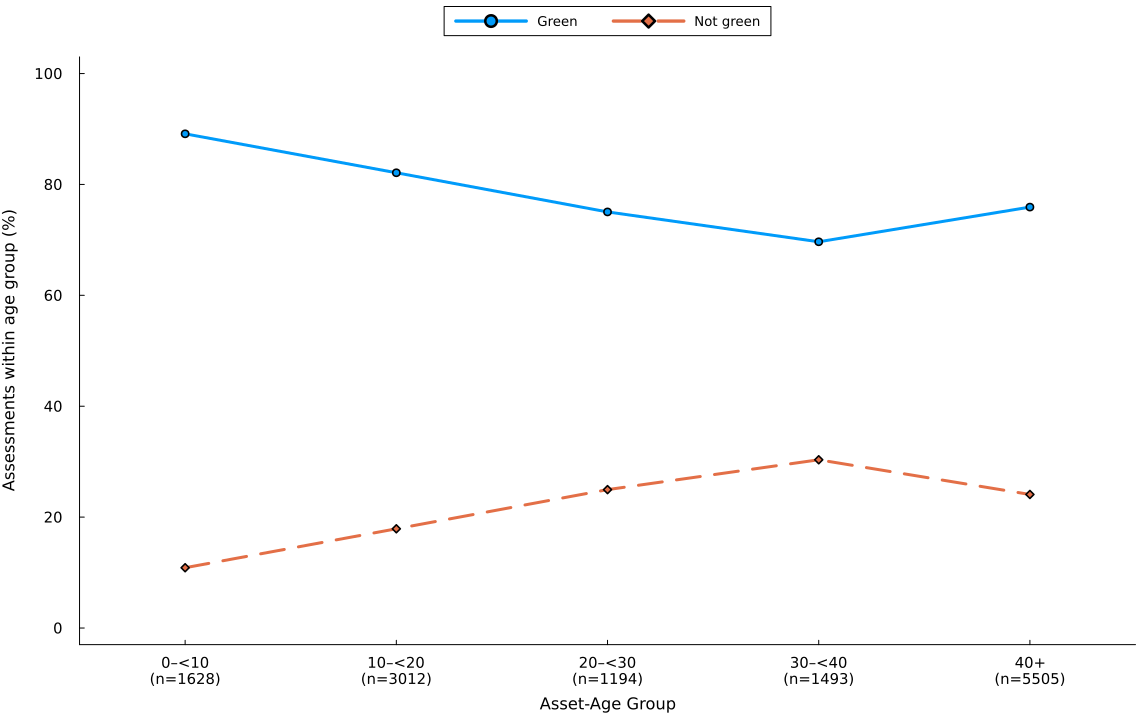
\includegraphics[width=0.95\linewidth]{interesting_plot2.png}
\caption{Assessment Condition by Asset Age.}
\label{fig:julian_plot2}
\end{figure}

\subsubsection{Condition Status Across Climate Categories}

Differences in assessed condition are also apparent across climate categories (Figure~\ref{fig:julian_plot3}). Relatively high proportions of not-green assessments are observed in Climate Codes 4 and 8, at approximately 50.0\% and 46.1\%, respectively, compared with only 12.4\% for Climate Code 7. Based on this variation, additional information may be provided by climate classification when evaluating component condition. However, climate data is limited across the dataset as a whole, with 6,514 of the 12,832 observations missing climate records and the remaining records unevenly distributed across only seven climate zones. Furthermore, the differences between categories may also reflect variations in asset age, maintenance history, or other characteristics. Further analysis is therefore necessary to determine whether climate contributes independently to condition prediction.

\begin{figure}[htbp]
\centering
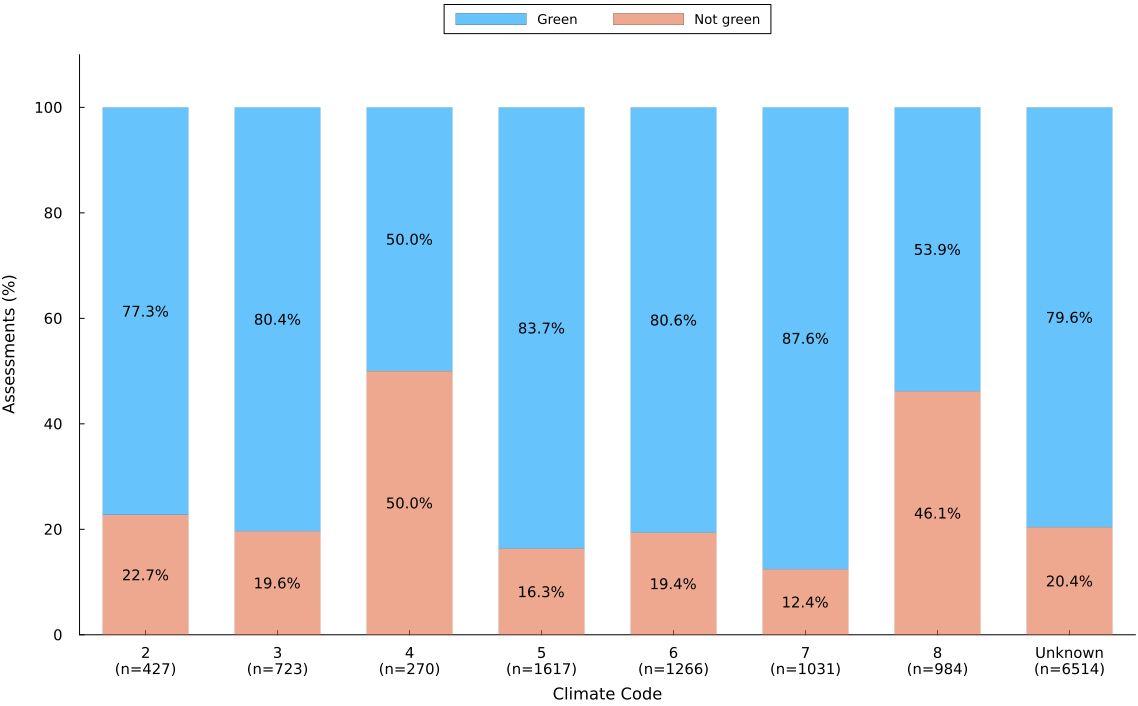
\includegraphics[width=0.95\linewidth]{interesting_plot3.png}
\caption{Assessment Condition by Climate.}
\label{fig:julian_plot3}
\end{figure}

\subsubsection{Seasonal Variation in Condition Status}

The climate comparison is extended by grouping assessments into winter, spring, summer, and fall to examine potential seasonal patterns in recorded condition (Figure~\ref{fig:julian_plot4}). For Climate Code 5, the proportion of not-green assessments increases from approximately 10.8\% during summer to 24.0\% during fall, indicating differences in condition distributions between assessment periods. Through similar comparisons across the remaining climate categories, a broader perspective is provided on how condition status varies throughout the year. Groups containing fewer than 50 observations are identified separately to avoid overinterpreting limited data. Assessment timing and asset characteristics, rather than direct environmental effects, may also be reflected by these seasonal differences.

\begin{figure}[htbp]
\centering
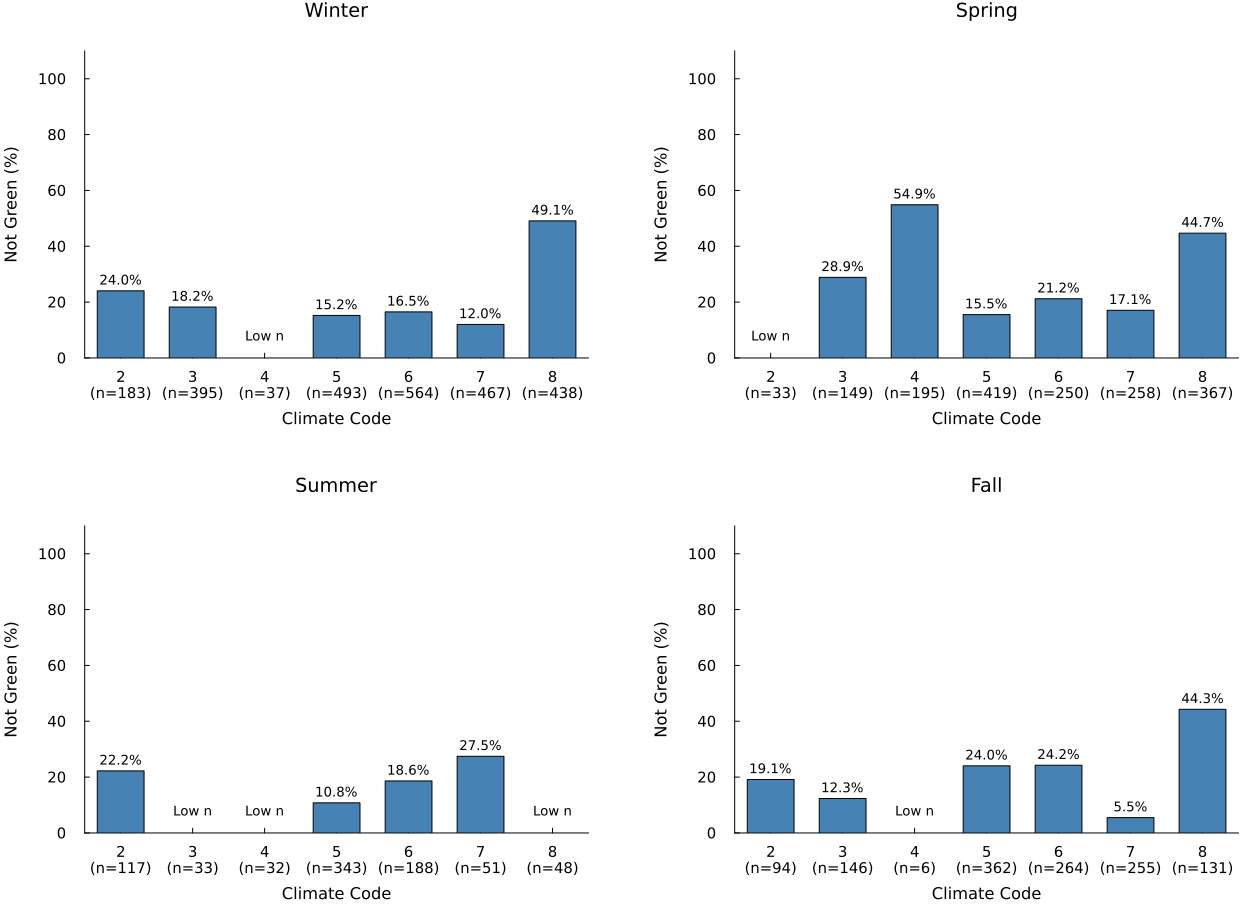
\includegraphics[width=0.95\linewidth,height=0.68\textheight,keepaspectratio]{interesting_plot4.png}
\caption{Not-Green Assessments by Season}
\label{fig:julian_plot4}
\end{figure}

\FloatBarrier

\subsection{Data Wrangling}

Following visualization and correlation analysis, the data were cleaned to prepare for further steps. Basic statistics of the raw dataset are shown in Table \ref{tab:boiler_descriptive_statistics}. Some columns such as Recency, Climate, and PrevScore have missing values. Additionally, some columns represent non-ordinal identifiers, and most of the ordinal columns are in mixed types and ranges varying by several orders of magnitude. To address these issues, the following data wrangling steps were performed. For Recency and PrevScore, the missing data represents components that have never previously been assessed. Since "Never Assessed" is potentially a valuable data point, a new column called "PrevAssessed" is created with a value of 0 or 1 representing whether a component has been assessed before. Missing values are then replaced with the mean of available data in both Recency and PrevScore, respectively. Similarly, for Climate, the missing data is simply missing data, with no underlying significance to its absence. Therefore, the missing fields are addressed by populating them with the mean of the known climate data.

\begin{table}[htbp]
\caption{Descriptive Statistics for Boiler Assessment Dataset Variables}
\label{tab:boiler_descriptive_statistics}
\centering
\small
\renewcommand{\arraystretch}{1.15}
\begin{tabular}{l r r r r r}
\hline\hline
\multicolumn{1}{c}{Variable} &
\multicolumn{1}{c}{Mean} &
\multicolumn{1}{c}{Minimum} &
\multicolumn{1}{c}{Maximum} &
\multicolumn{1}{c}{Missing} &
\multicolumn{1}{c}{Unique Values} \\
\hline
Id                & 4,673.27 & 1     & 9,334   & 0     & 9,334 \\
Spec              & 55.97    & 1     & 110     & 0     & 110 \\
System            & 1.00     & 1     & 1       & 0     & 1 \\
MEC               & 1.00     & 1     & 1       & 0     & 1 \\
DesignLife        & 30.00    & 15    & 30      & 0     & 2 \\
Qty               & 1.01     & 1     & 6       & 0     & 5 \\
UOM               & --       & Each  & Each    & 0     & 1 \\
Year              & 2020.91  & 2011  & 2025    & 0     & 15 \\
Month             & 5.64     & 1     & 12      & 0     & 12 \\
NormalizedAge     & 0.42     & 0.00  & 4.00    & 0     & 85 \\
EffectiveAge      & 16.72    & 0.00  & 121.00  & 0     & 84 \\
RSL               & 16.47    & -90.00& 30.00   & 0     & 278 \\
Recency           & 3.53     & 0.00  & 10.00   & 9,334 & 10 \\
Climate           & 5.52     & 2     & 8       & 6,514 & 7 \\
PredictedCI       & 76.48    & 0.00  & 100.00  & 0     & 435 \\
Score             & 84.78    & 10    & 100     & 0     & 16 \\
CRV               & 81,294.00& 6,290 & 902,540 & 0     & 965 \\
Fac               & 71.86    & 1     & 134     & 0     & 134 \\
AssetAge          & 38.75    & 0     & 181     & 0     & 154 \\
AssetDesignLife   & 51.12    & 30    & 60      & 0     & 11 \\
PrevScore         & 85.82    & 10    & 100     & 9,334 & 14 \\
\hline\hline
\end{tabular}
\end{table}

Next, a new column is created called NormalizedAssetAge set to AssetAge / AssetDesignLife for consistency with the convention used for NormalizedAge of the component. For Month, to capture the impact of seasons on assessment scores, the variable is modified in a way that keeps the cyclical nature of seasons intact. Two new columns are created (MonthSin and MonthCos) representing the Month in a circular projection and keeping months, like December and January, close together ordinally. To address the large magnitude difference for Component Replacement Value (CRV), a new column is created called LogCRV representing the log of the original CRV values. Through this transformation, the scale is brought to a more comparable space and a more symmetric distribution is produced, as shown in Figure \ref{fig:crv_log}. 

%Finally, Id, Spec, System, MEC, UOM, Fac, Qty, DesignLife, Month, AssetAge, and AssetDesignLife are omitted from the PCA analysis due to either being non-ordinal identifier columns, having the same value across nearly all the dataset (Qty, DesignLife), or having alternative suitable representations from the previous wrangling steps. Score is also omitted as the dependent variable, avoiding data leakage when analyzing potential predictive features.

\begin{figure}
\centering
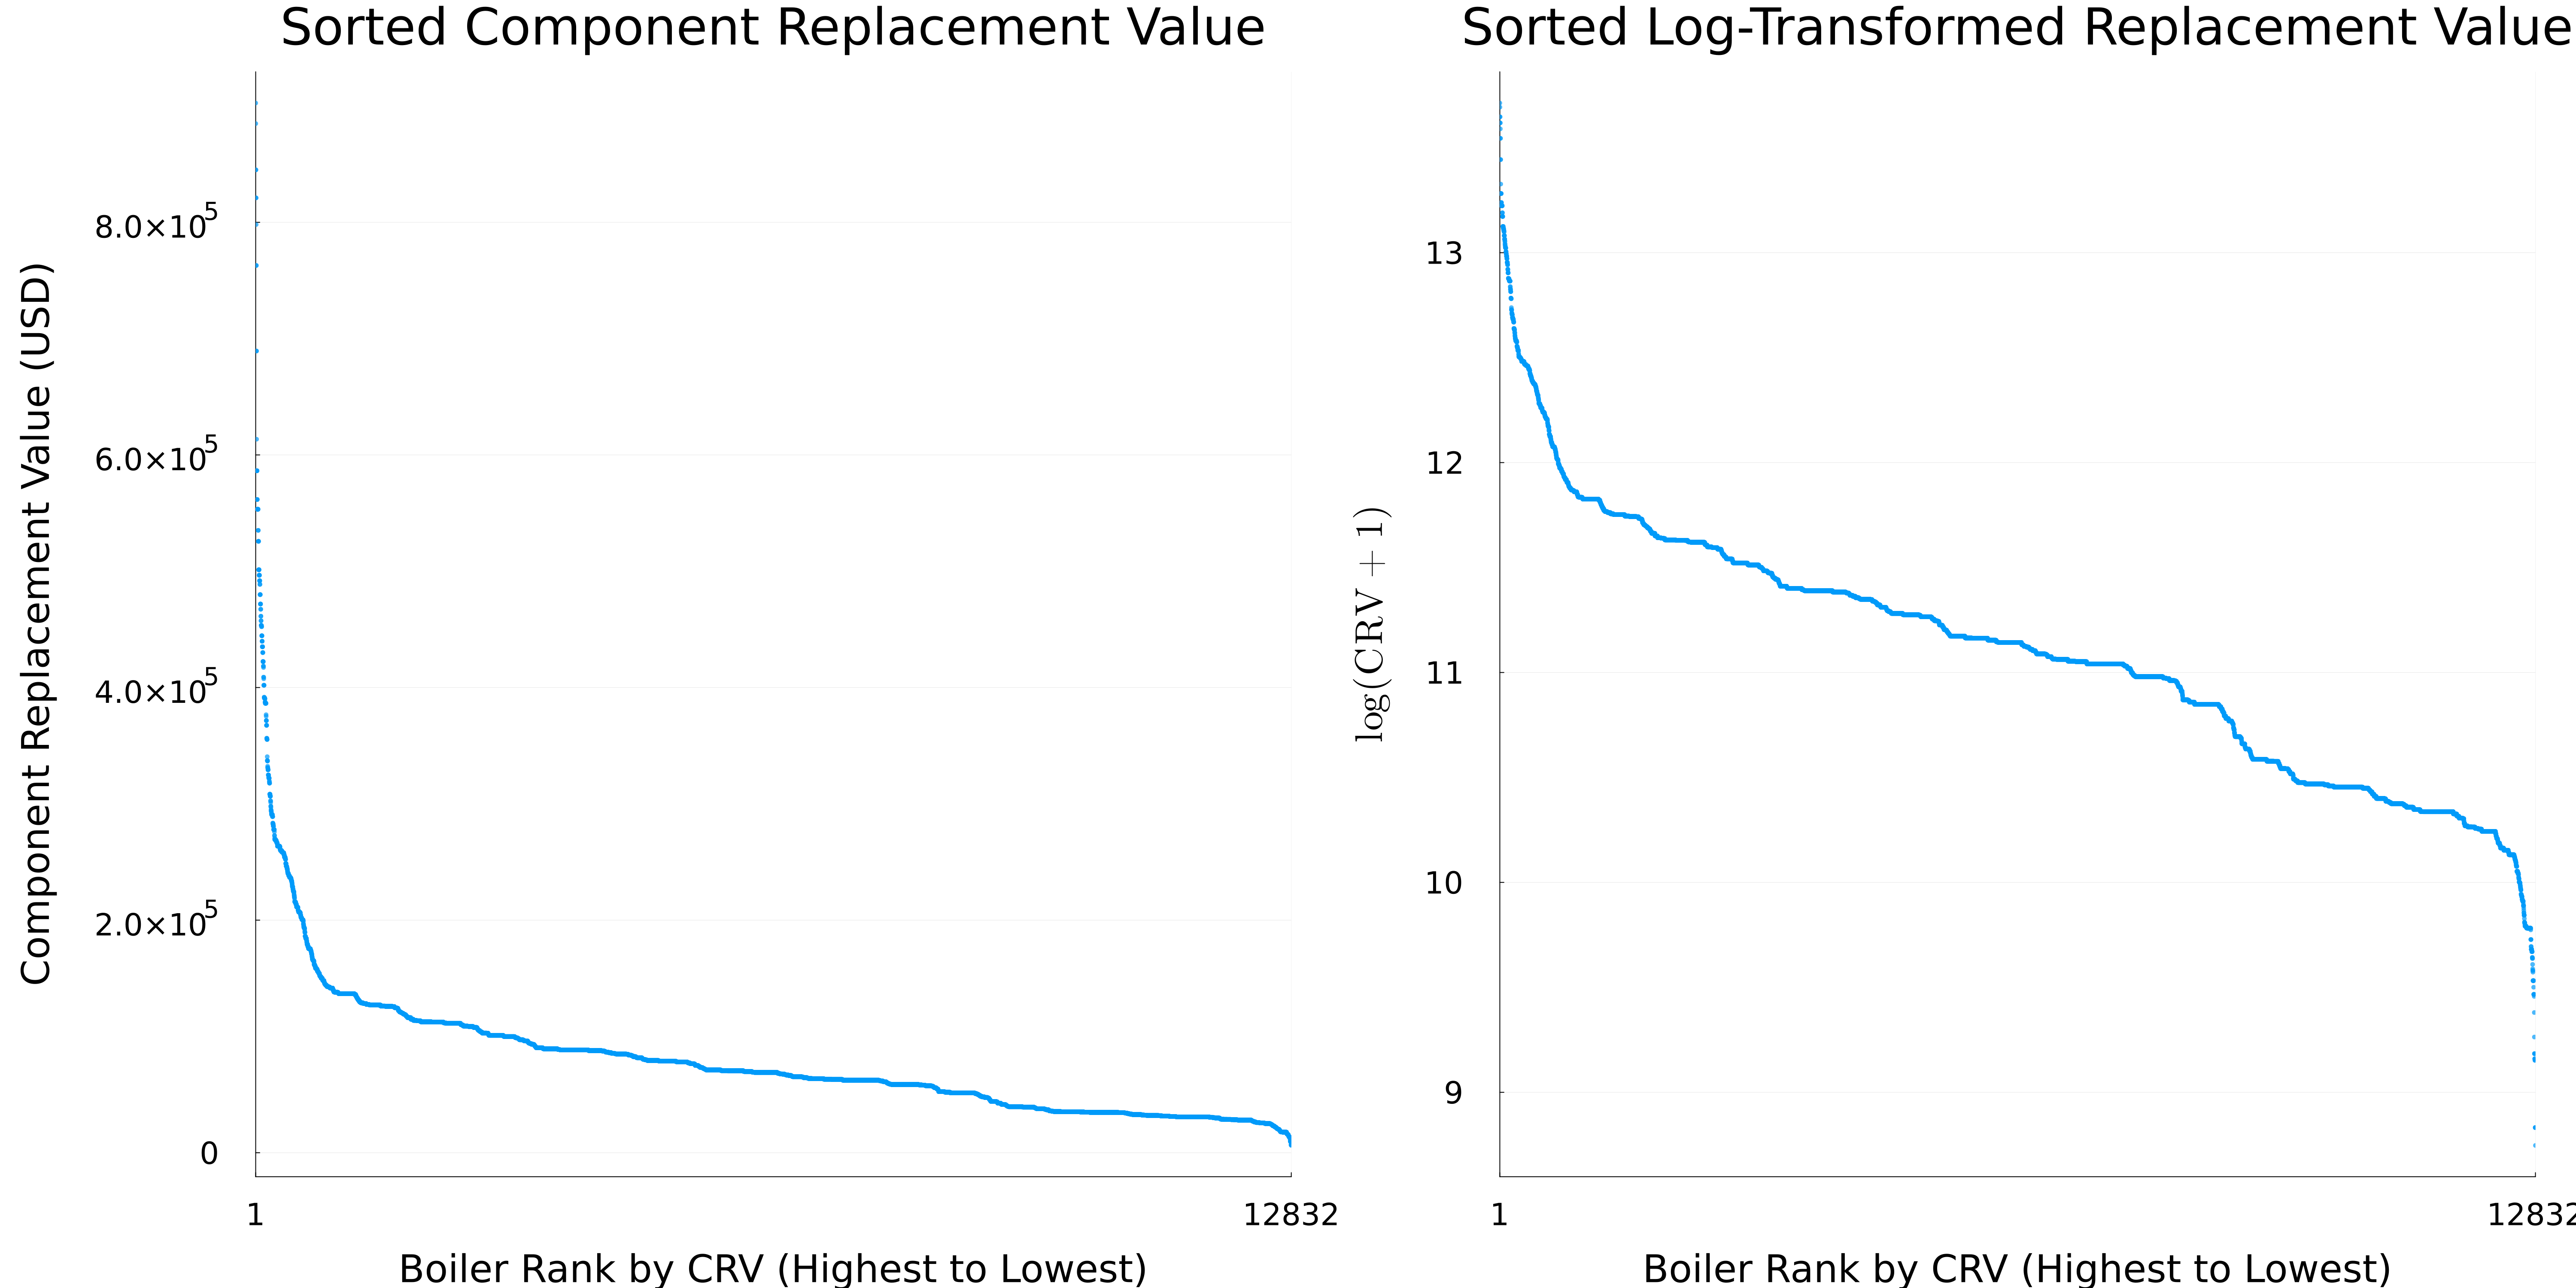
\includegraphics[width=1\linewidth]{log_crv_scatter.png}
\caption{Conversion of CRV to LogCRV}
\label{fig:crv_log}
\end{figure}

\subsection{Principal Component Analysis}

After data wrangling, a PCA was performed using the following columns of the cleaned dataset: NormalizedAge, EffectiveAge, RSL, PredictedCI, Recency, PrevScore, PrevAssessed, NormalizedAssetAge, LogCRV, Year, MonthSin, MonthCos, and Climate. First, data were normalized and standardized (by centering on the mean, then dividing by standard deviation). Then, the singular value decomposition (SVD) was generated. The initial explained variance by principal component is shown in Figure \ref{fig:pca_init}. Principal component (PC) 1 has a notable dominance of 34\% of the explained variance. Upon inspection of PC 1, all similarly derived lifecycle parameters (NormalizedAge, RSL, PredictedCI, and EffectiveAge) have roughly equal absolute values of $\sim$.49 and are therefore relatively redundant. A new version of the PCA was then run using a single lifecycle parameter, RSL. RSL was selected because it is an intuitively interpretable value. Through this reduced-parameter PCA, a smoother decline in explained variance across the PCs was produced, as seen in Figure \ref{fig:pca_reduced}.

\begin{figure}
\centering
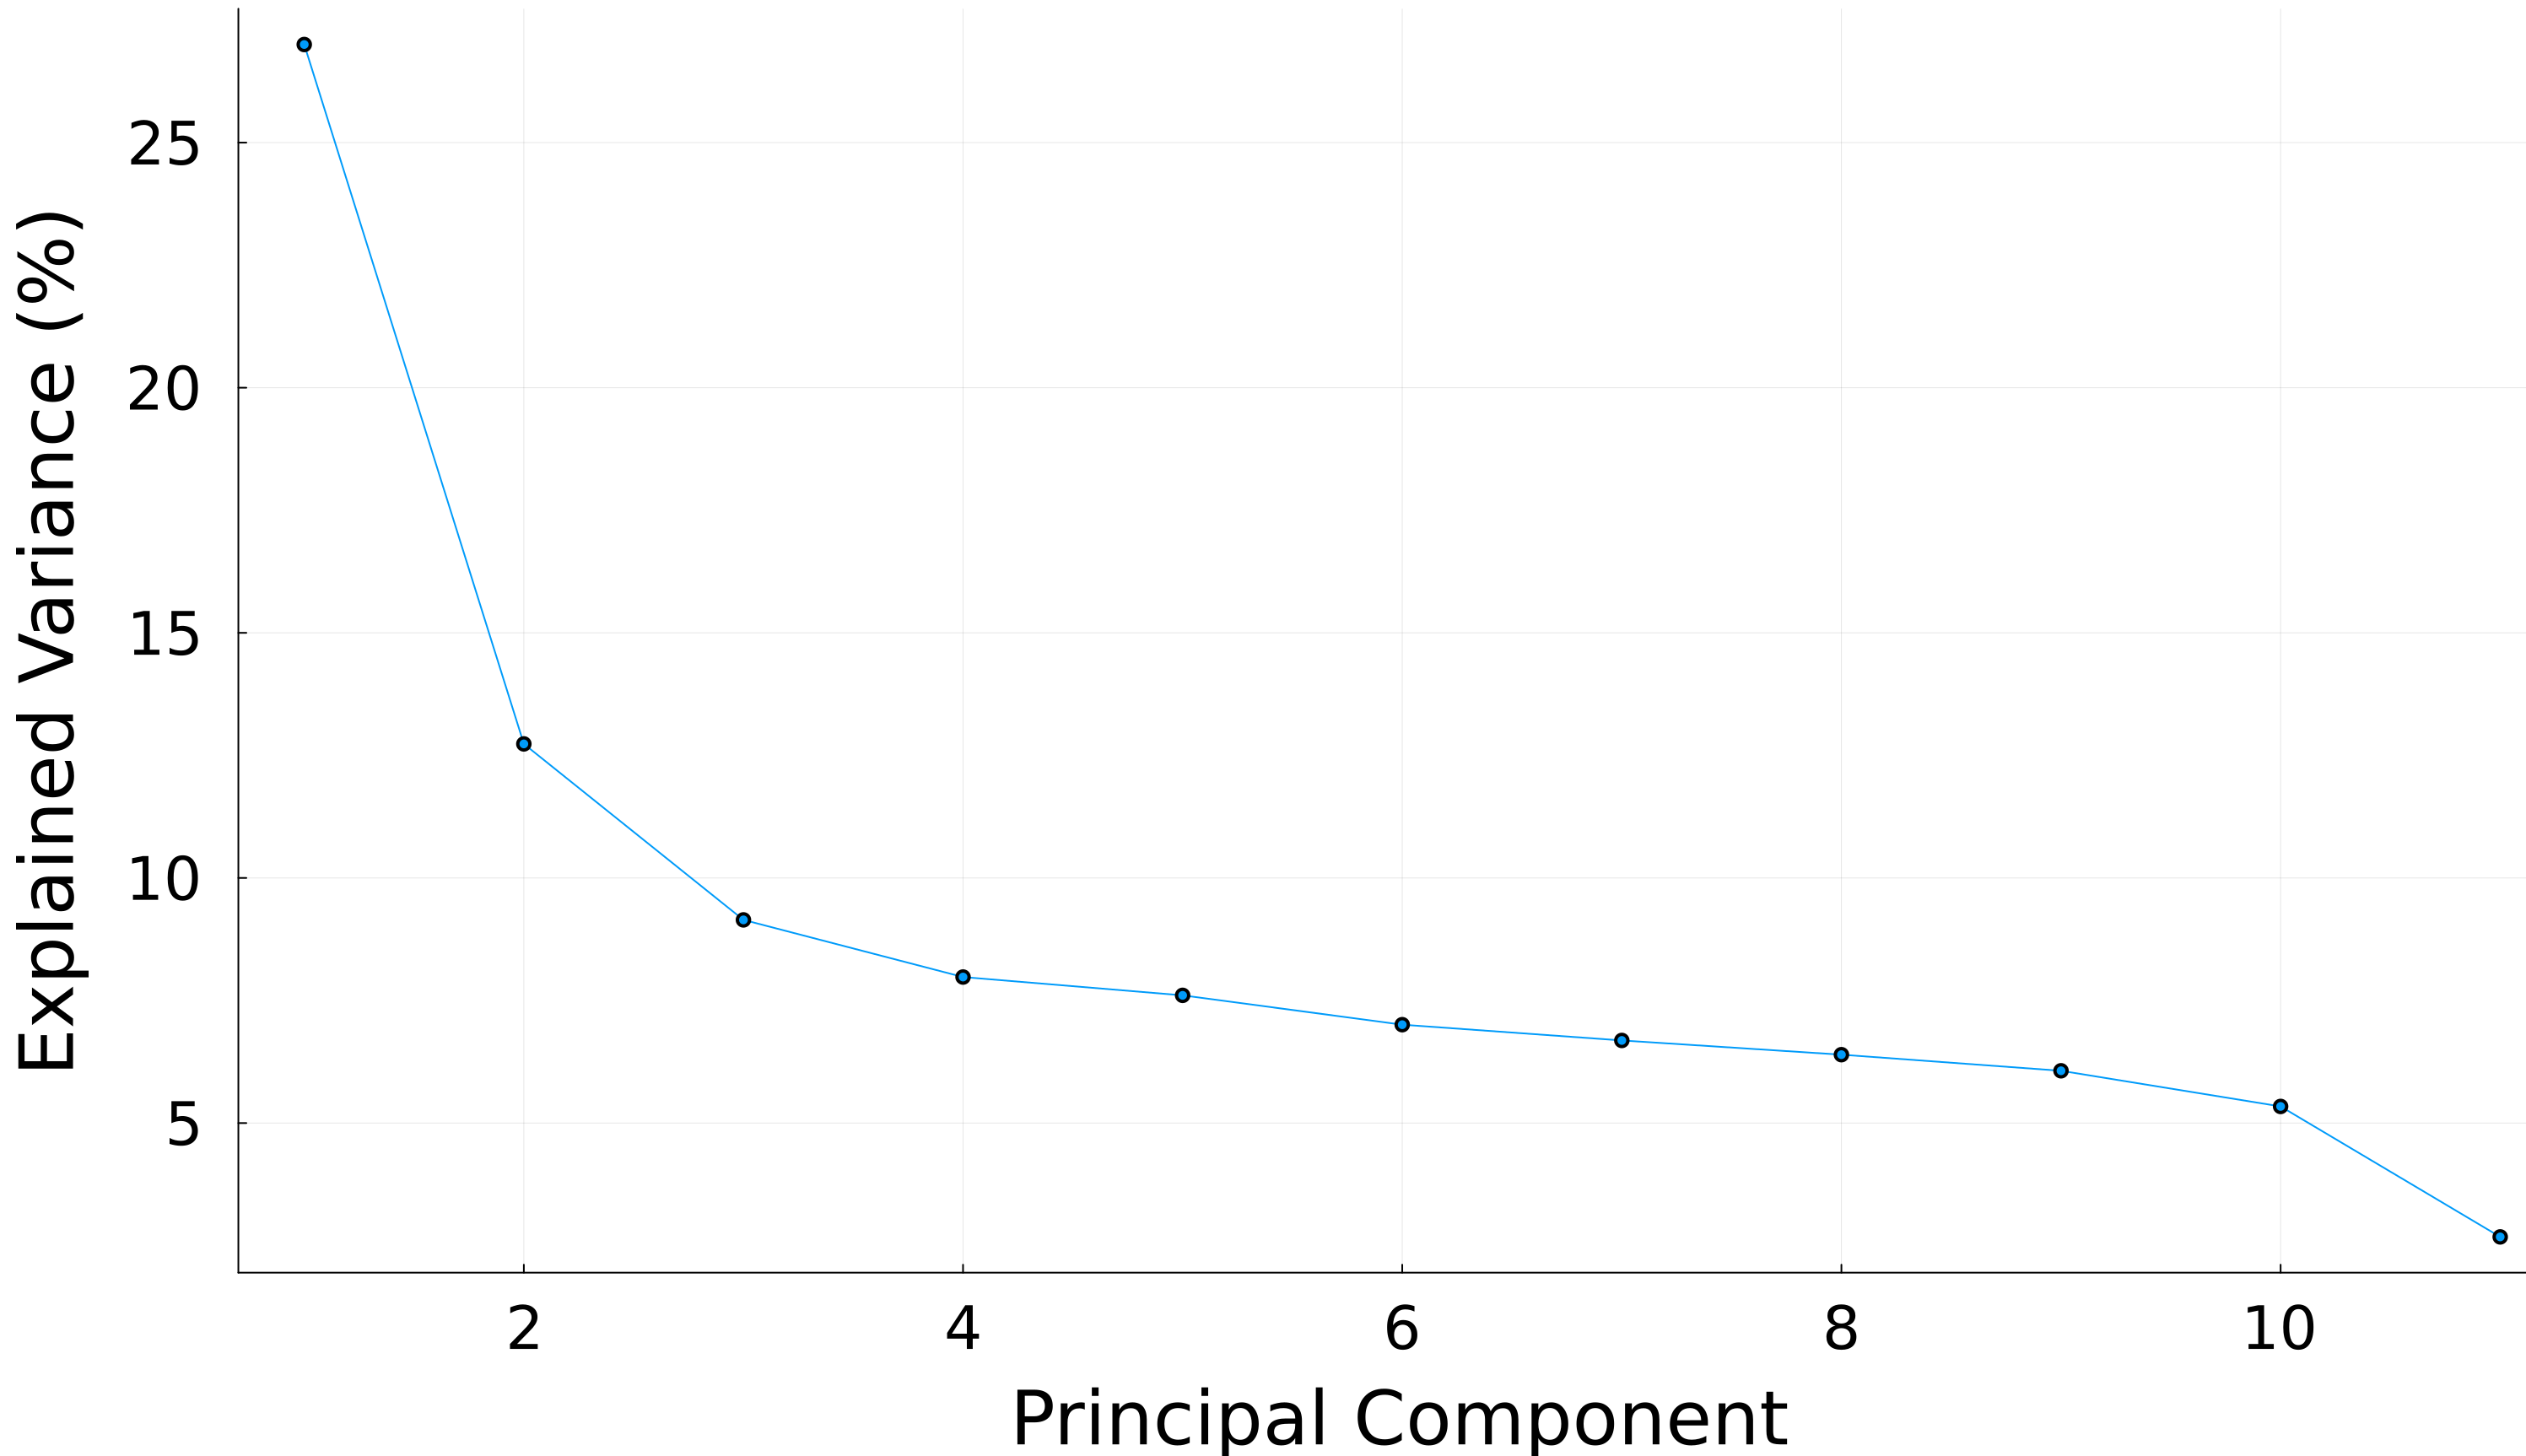
\includegraphics[width=.8\linewidth]{pca_plot_initial.png}
\caption{Initial PCA Variance}
\label{fig:pca_init}
\end{figure}

\begin{figure}
\centering
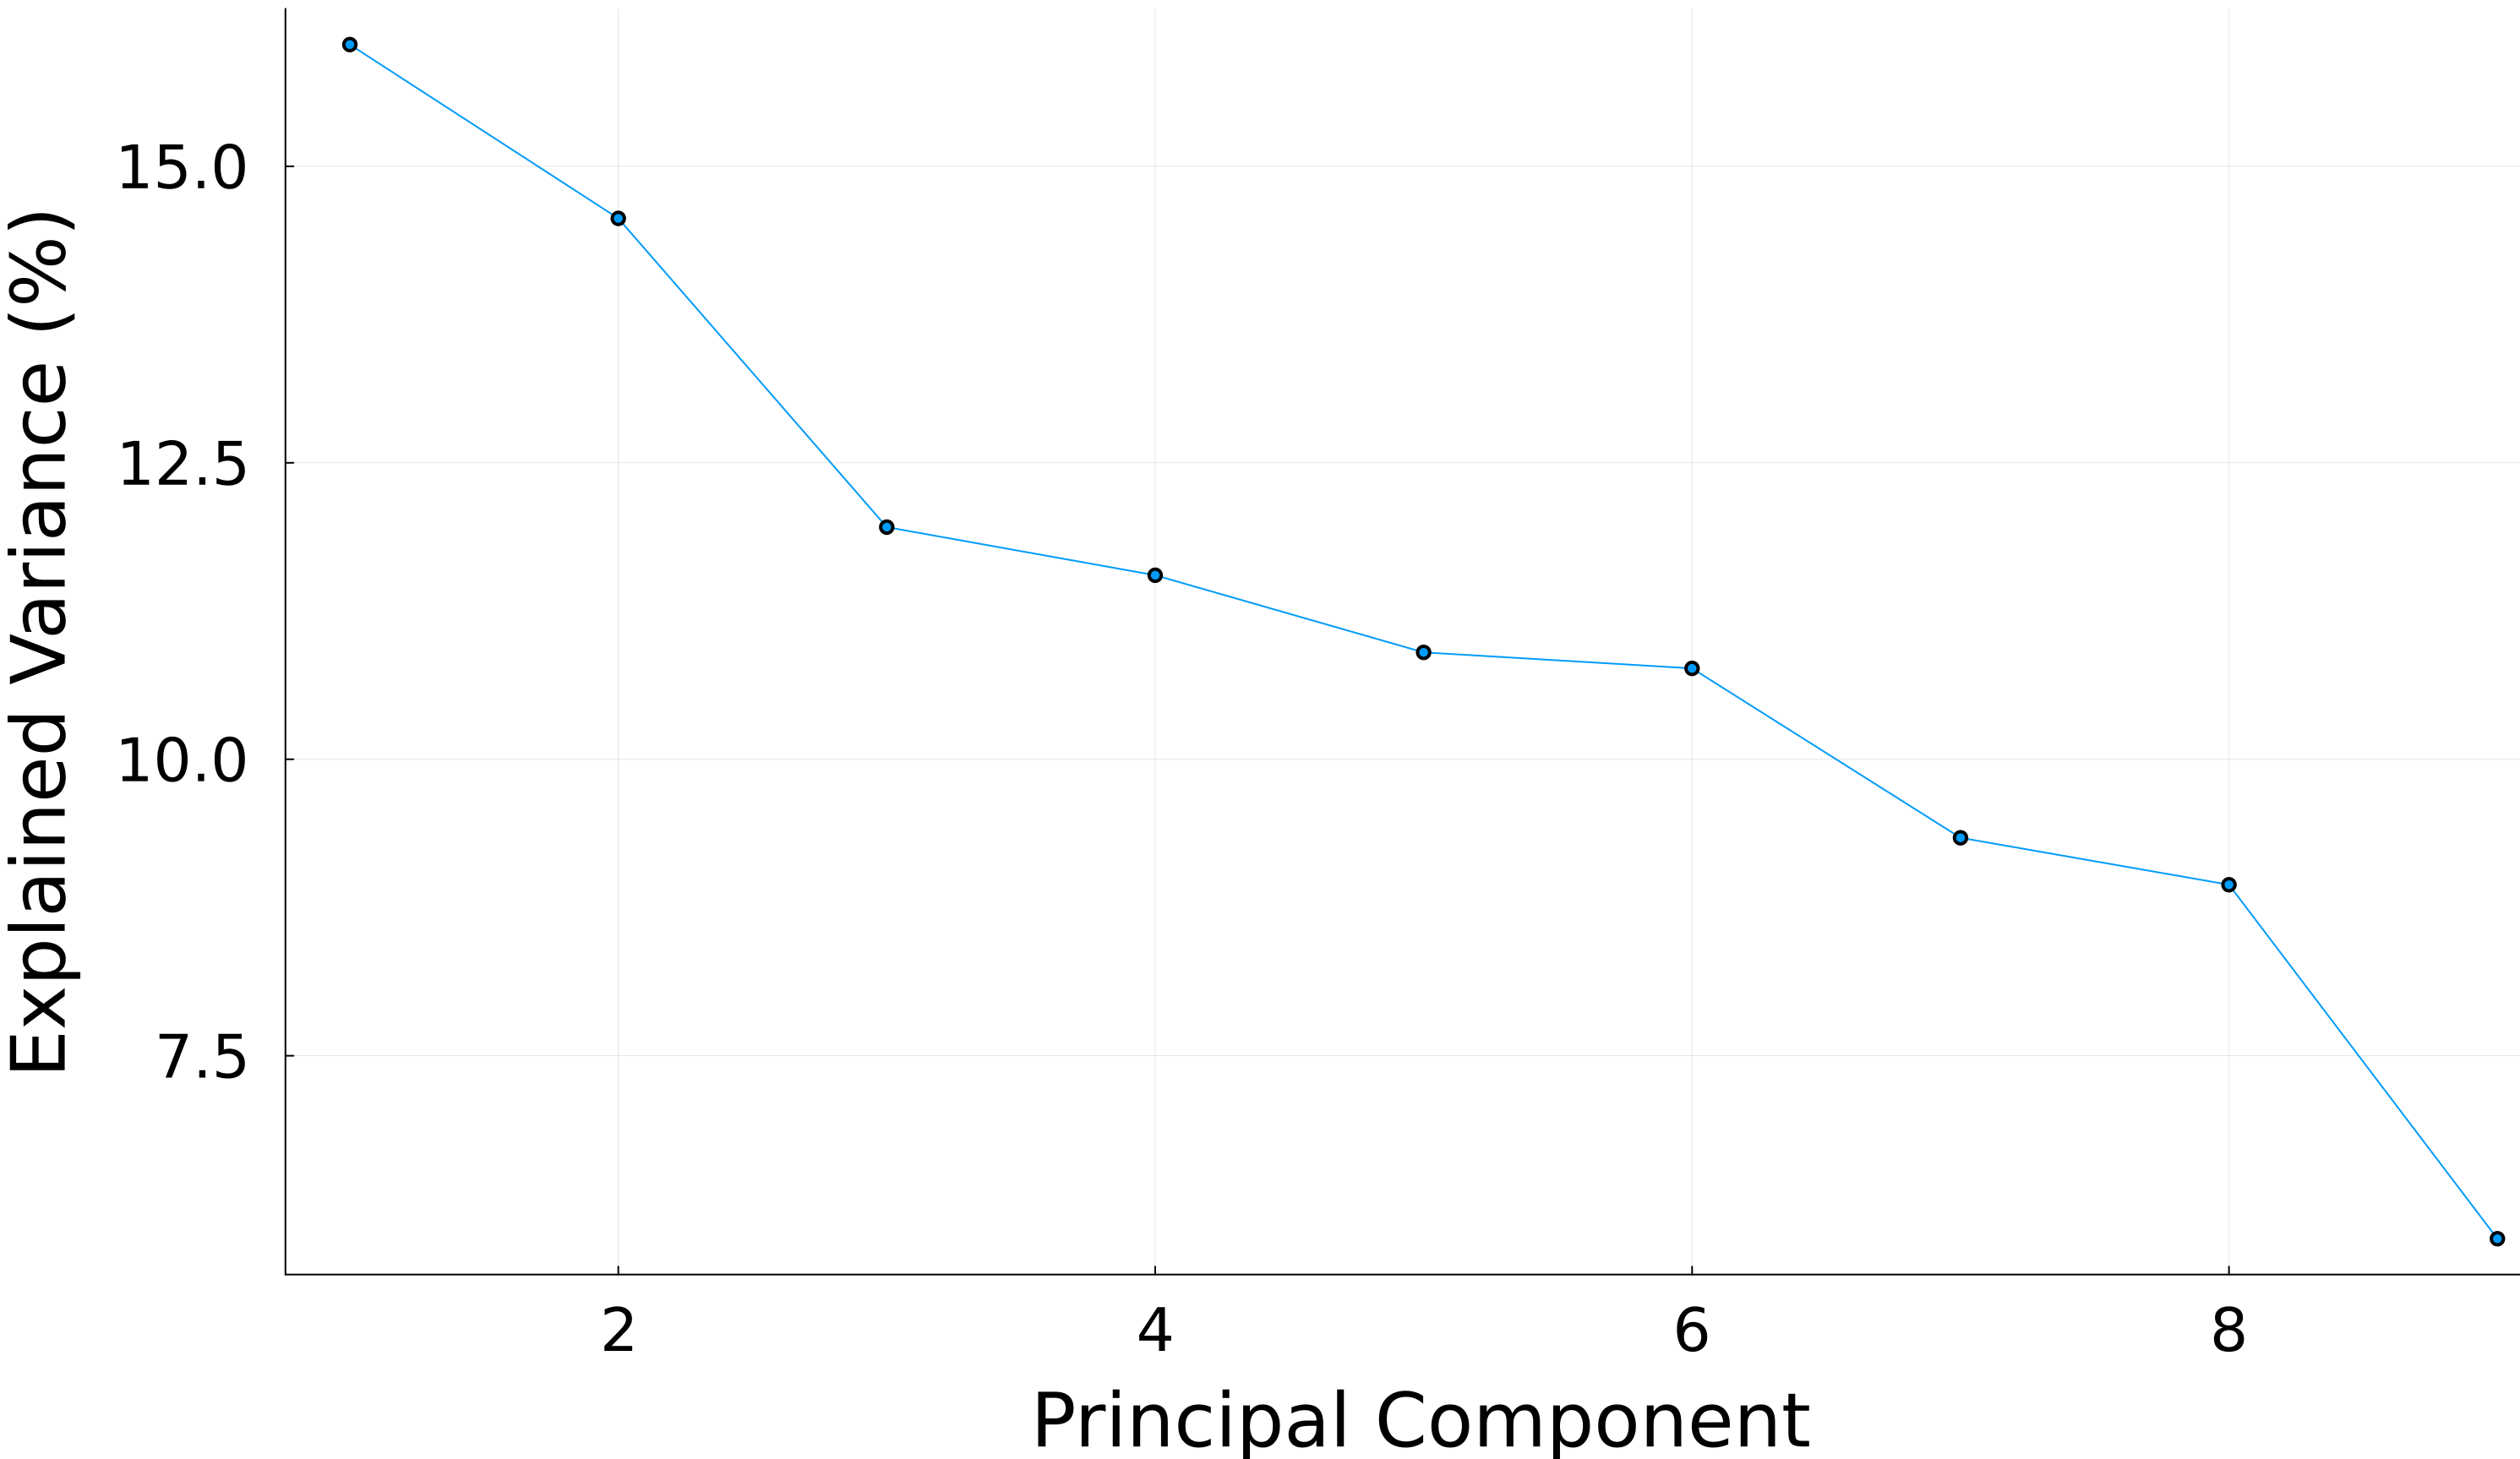
\includegraphics[width=.8\linewidth]{pca_plot_reduced.png}
\caption{Reduced Parameter PCA Variance}
\label{fig:pca_reduced}
\end{figure}

In the loadings heatmap of the reduced parameter PCA (Figure \ref{fig:heatmap_reduced_pca}), the expected dominance of RSL is still observed in the first PC, while Recency, Climate, and Month are also key to PCs 2 and 3. To search for potential predictability, PC observation mode ($V^T$) values were mapped back to assessed scores, color coded by "Green Region" ($\mathrm{Score} \geq 85$) and "Not Green Region" ($\mathrm{Score} < 85$), and then plotted in histograms for each PC in search of distinguishing characteristics (See Figure \ref{fig:rsl_no_pgreen}). PC 1 histograms were produced with various trial-and-error parameter sets, attempting to further identify combinations that better separated Green and Not Green regions. Through these trials, the two-peaked distribution in the Green data was removed by reintroducing PredictedCI (in addition to RSL), resulting in more offset normal distributions (Figure \ref{fig:rsl_ci_no_pgreen}). Additionally, better separation was observed when omitting PrevScore and Recency, whereas observably better separation was produced when using PrevAssessed alone. PrevScore, Recency, and PrevAssessed are linked, similar to the lifecycle parameters, although it is unclear as to why better separation between clusters was produced by the simple boolean of PrevAssessed. This could possibly be an artifact of the starting point of assessment history targeting a variably aged portfolio.

\begin{figure}
\centering
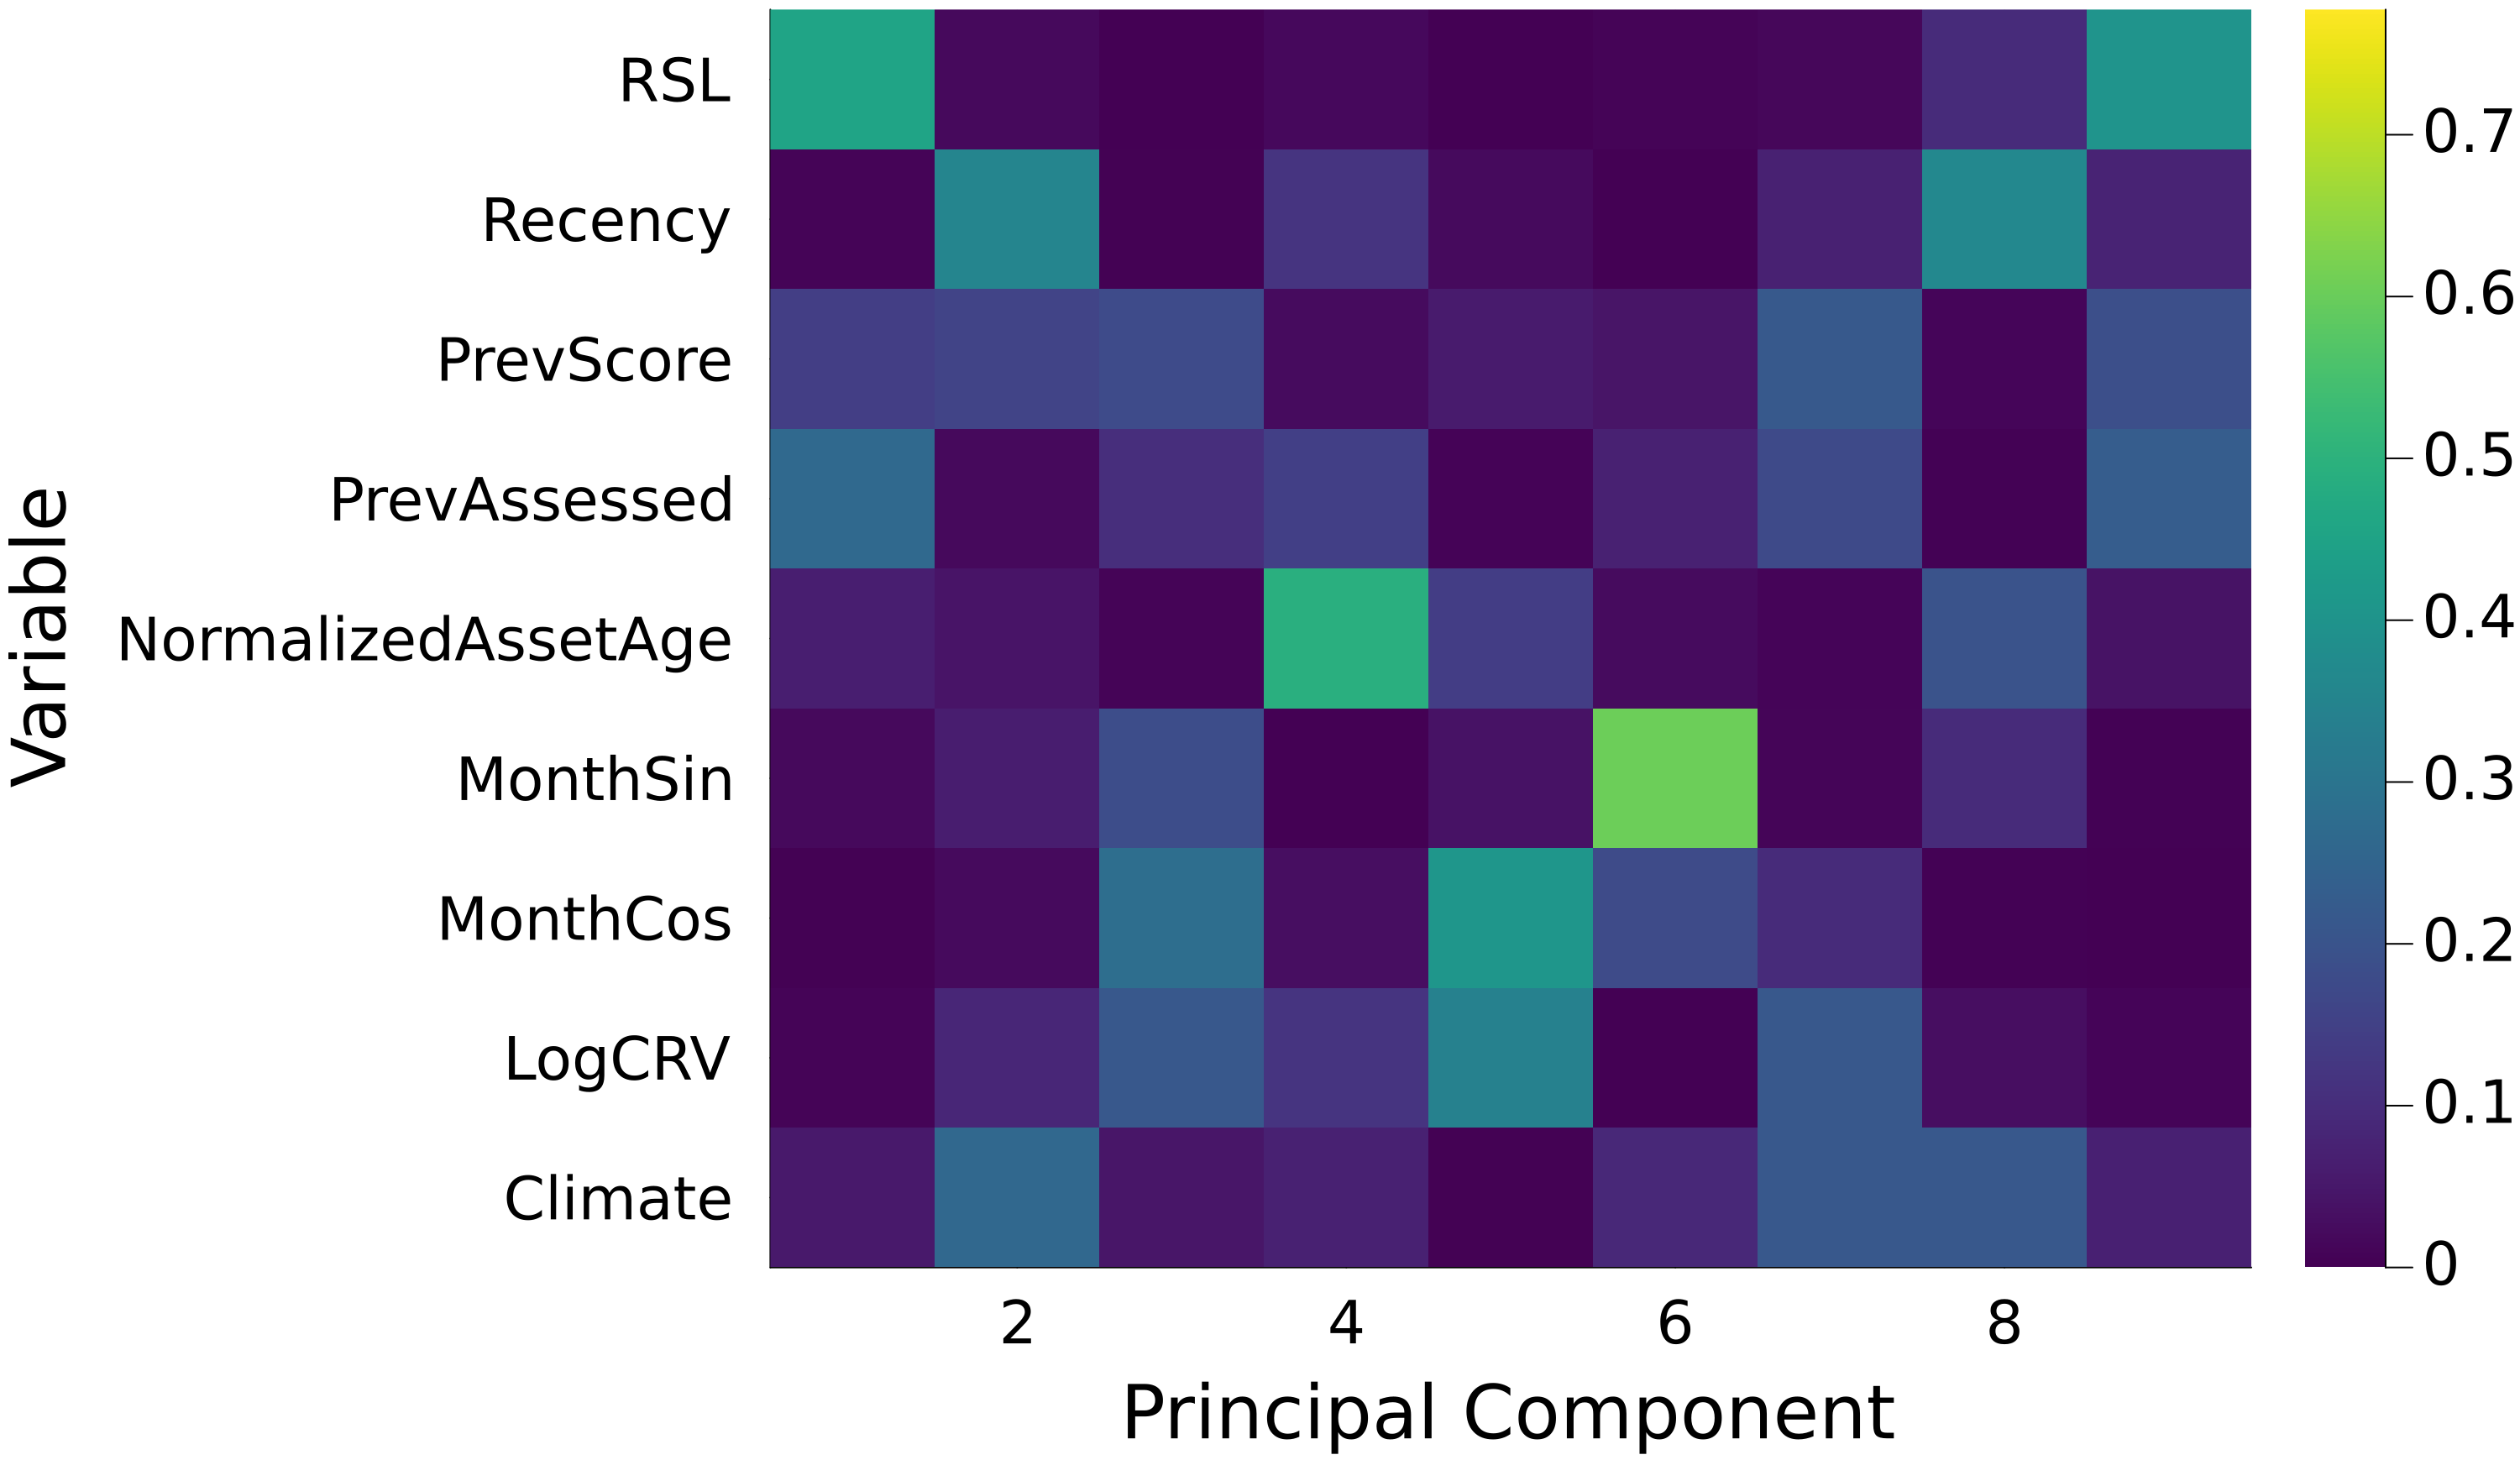
\includegraphics[width=.8\linewidth]{loadings_heatmap_reduced_pca.png}
\caption{Loadings Heatmap for Reduced Parameter PCA}
\label{fig:heatmap_reduced_pca}
\end{figure}

\begin{figure}
\centering
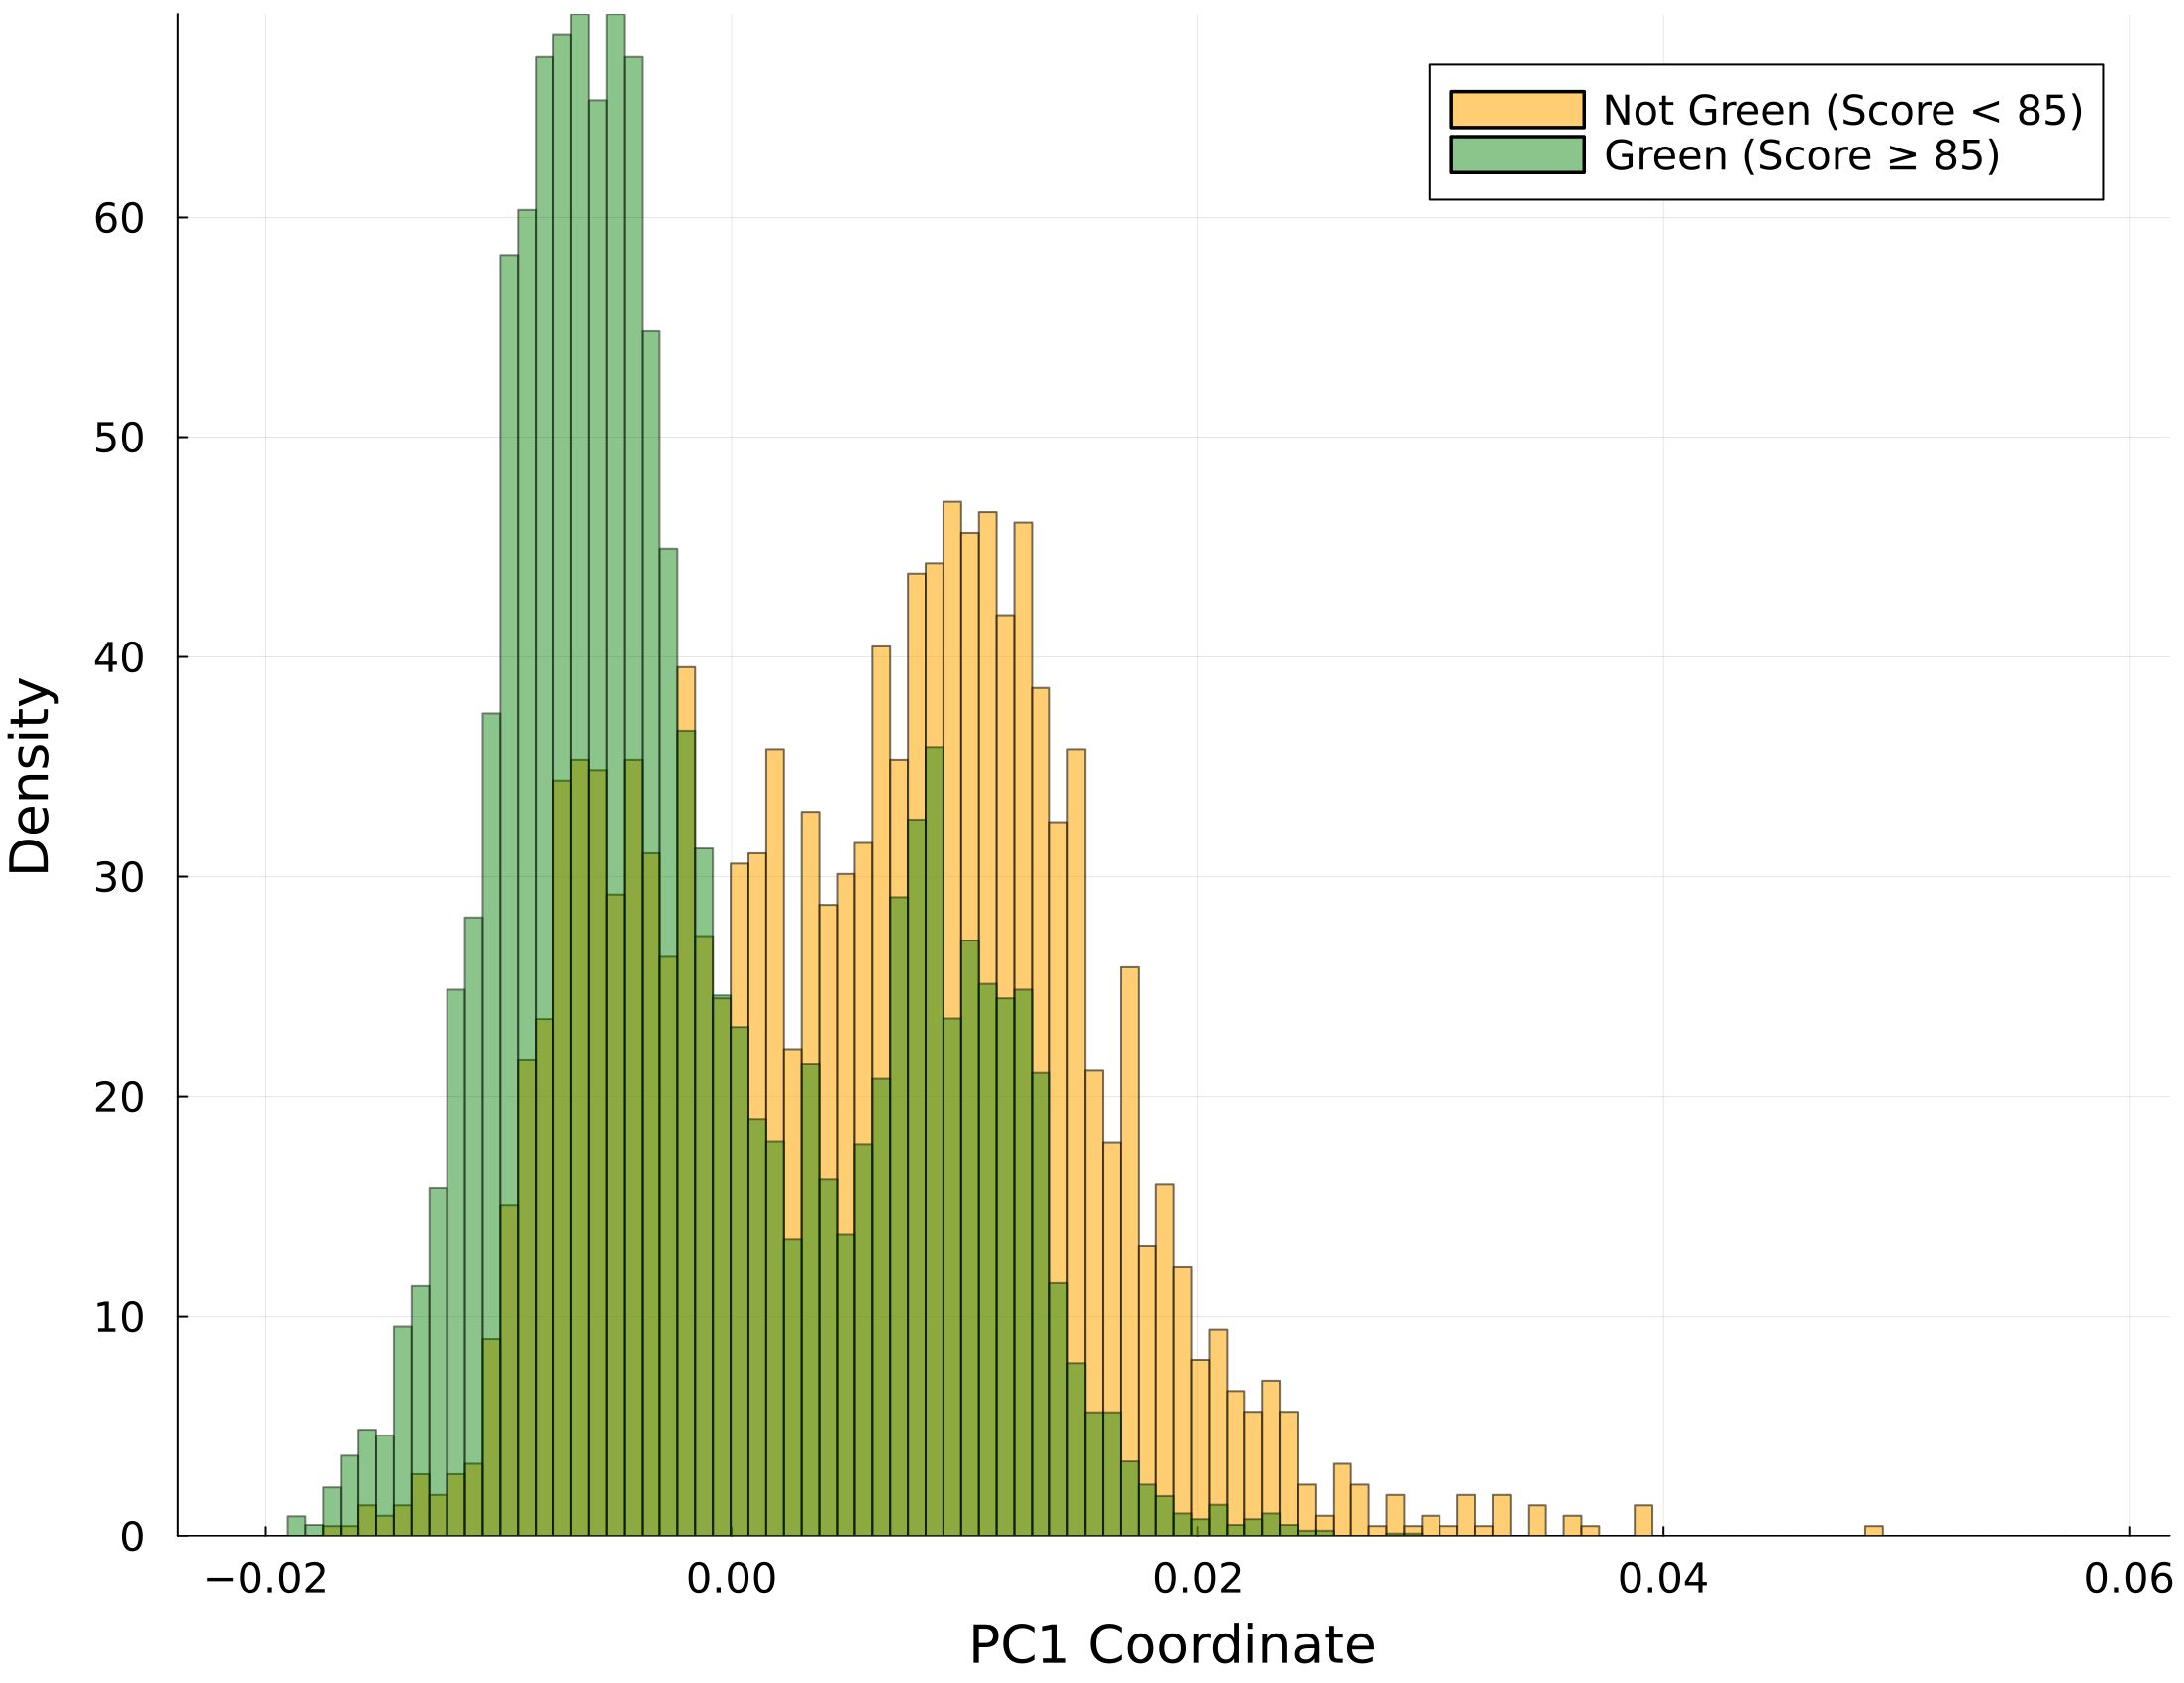
\includegraphics[width=.8\linewidth]{RSL_no_PGreen.png}
\caption{PC1 with RSL, PrevAssessed, LogCRV, MonthSin, MonthCos, NormalizedAssetAge}
\label{fig:rsl_no_pgreen}
\end{figure}

\begin{figure}
\centering
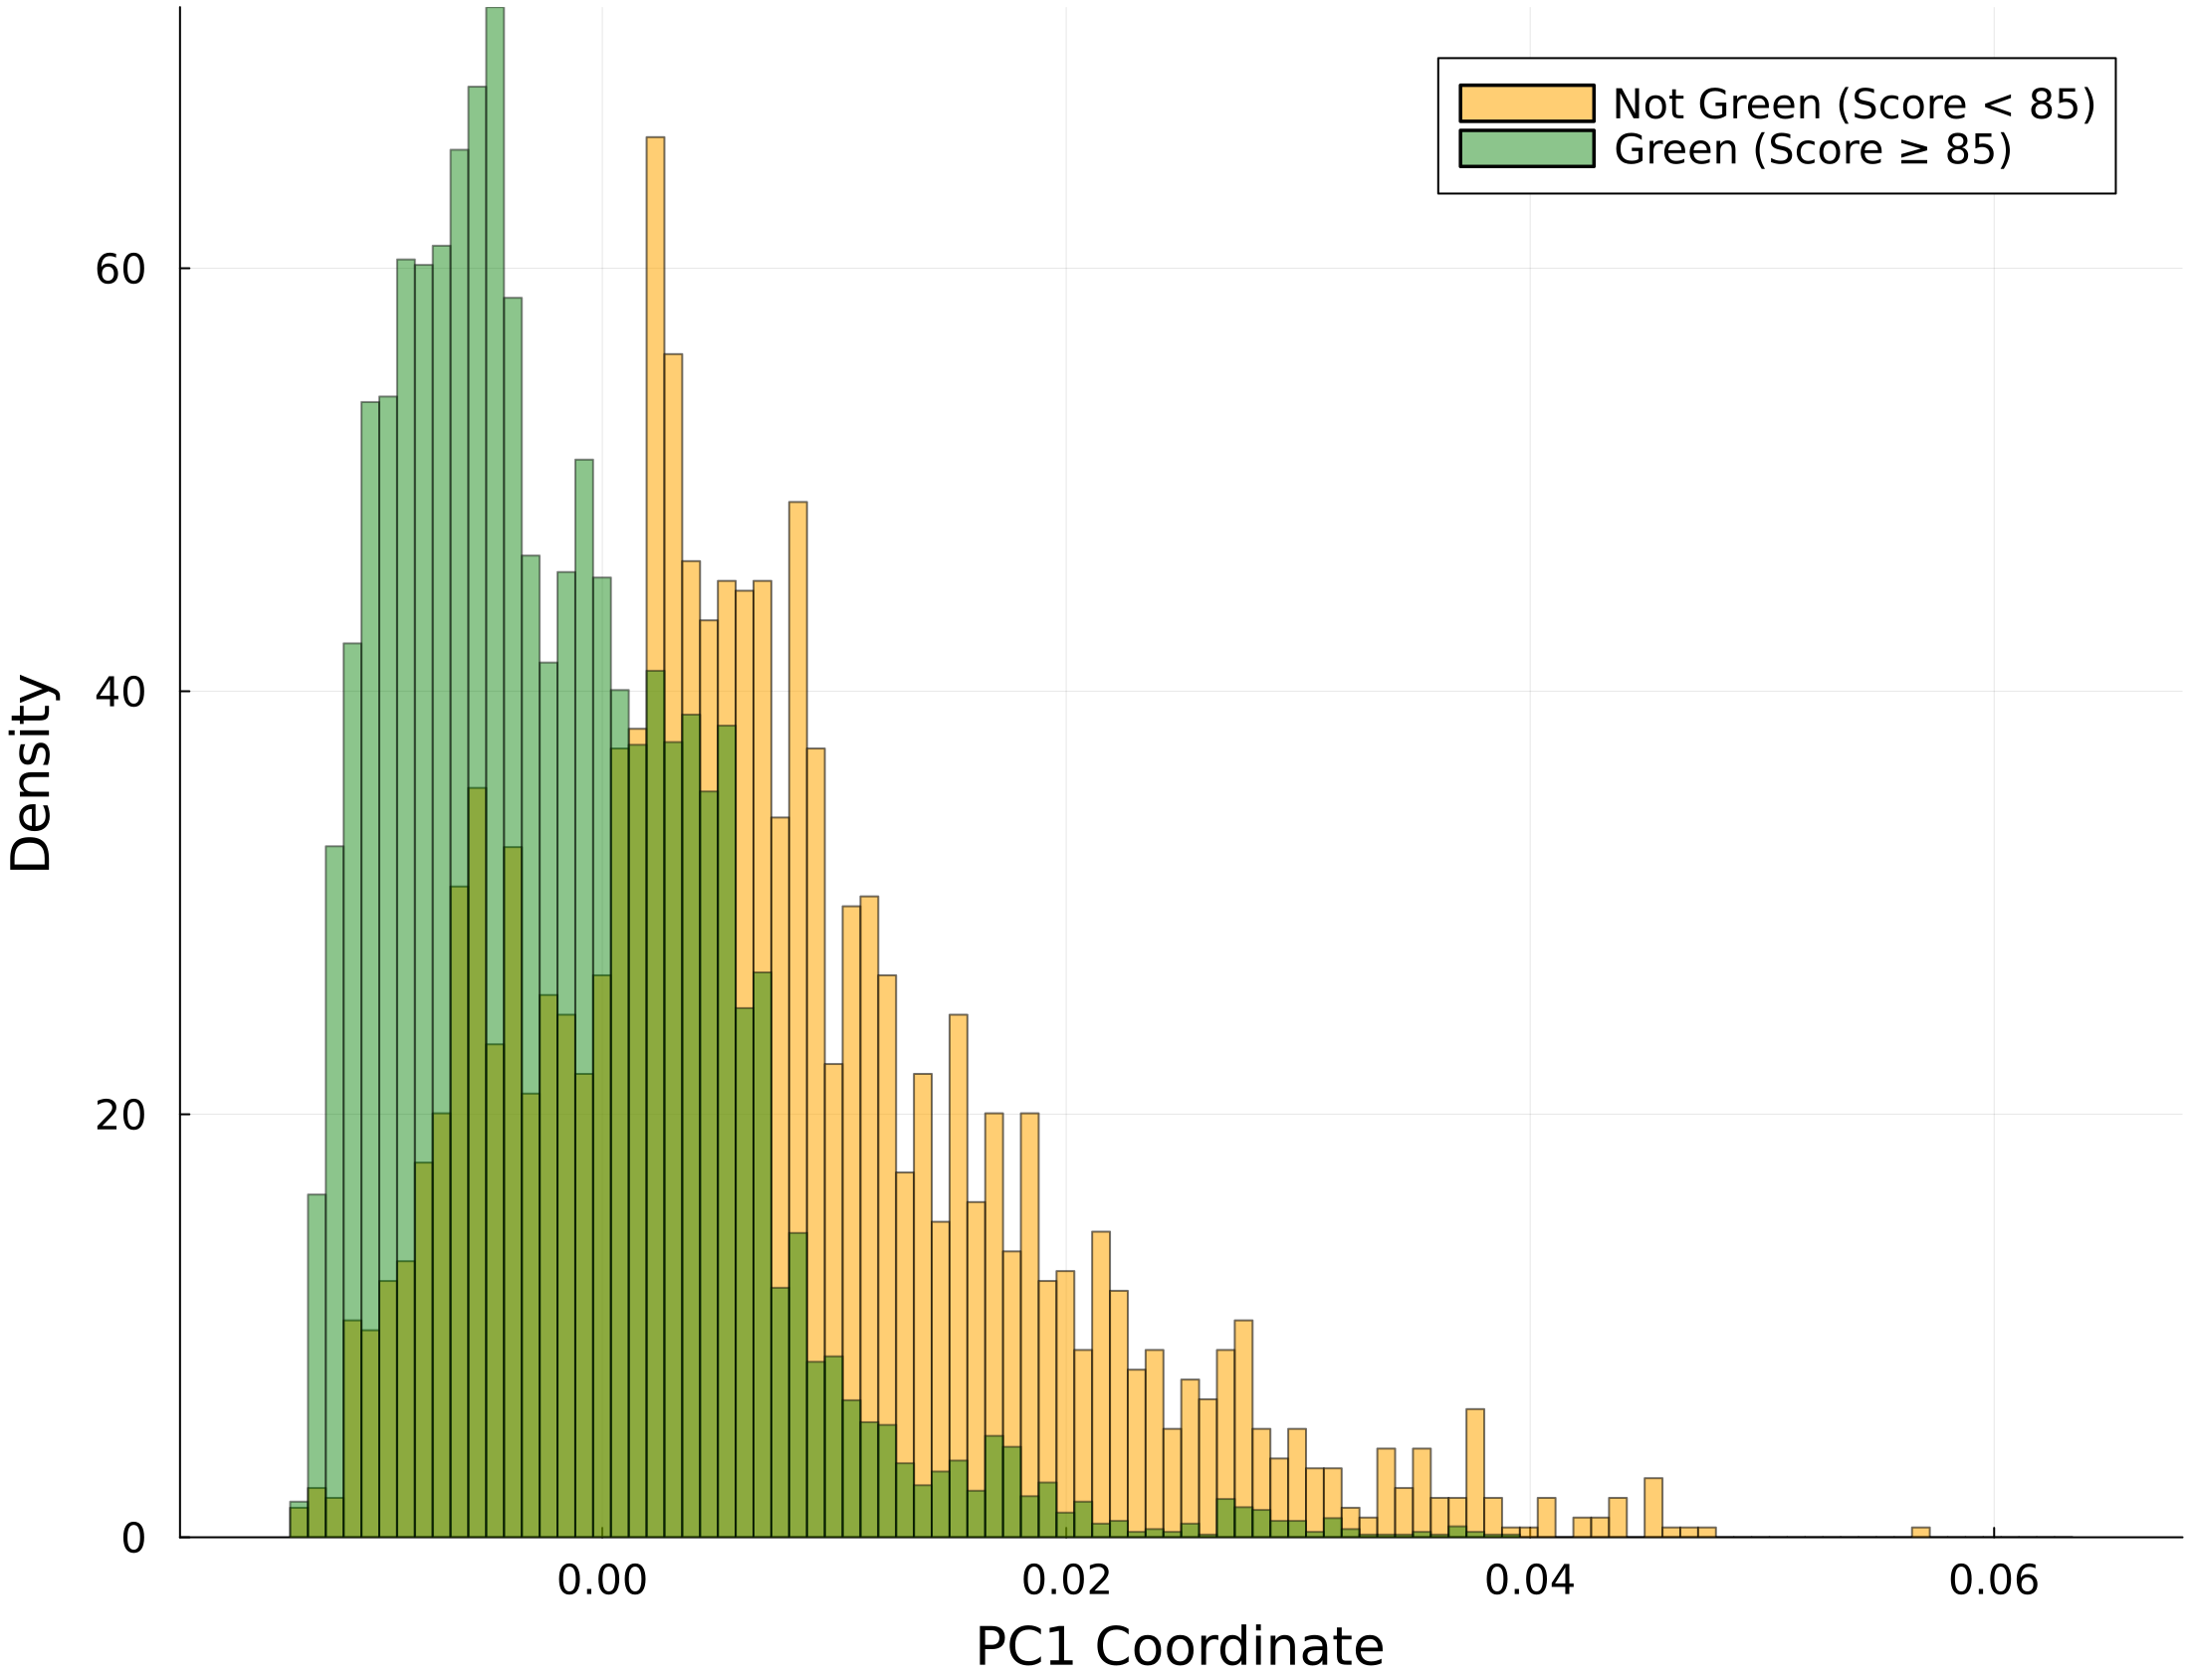
\includegraphics[width=.8\linewidth]{RSL_CI_no_PGreen.png}
\caption{PC1 with RSL, PredictedCI, PrevAssessed, LogCRV, MonthSin, MonthCos, NormalizedAssetAge}
\label{fig:rsl_ci_no_pgreen}
\end{figure}

Together, the findings from this exploratory analysis establish the baseline feature set and modeling considerations. Because a boiler's condition Score cannot be predicted by any single variable correlation and a strong relationship exists between the lifecycle parameters, predictive modeling is initialized using the following reduced feature set: lifecycle parameters limited to RSL and PredictedCI, assessment history represented solely by PrevAssessed, and the wrangled asset and environmental features (NormalizedAssetAge, MonthSin, MonthCos, LogCRV, and Climate).

\FloatBarrier

\section{Preliminary Modeling}

\subsection{Multiple Linear Regression Modeling}

Three types of linear regression models were constructed to predict a boiler's Score, treated as a continuous variable, using the independent variables in the wrangled dataset (RSL, PredictedCI, PrevAssessed, NormalizedAssetAge, MonthSin, MonthCos, LogCRV, and Climate). All regression models were constructed using Julia's MLJ package.

The same model form was used for ordinary least squares (OLS), Ridge, and Lasso regression:
\[
y = \beta_0 + \beta_1 x_1 + \beta_2 x_2 + \dots + \beta_p x_p + \epsilon,
\]
where $y$ is the observed Score, $\beta_j$ are regression coefficients, $x_j$ are independent variables, and $\epsilon$ is a random error term. The squared $L_2$ norm of the residuals was minimized for OLS. A squared $L_2$ norm regularization term was added to the objective function for Ridge regression, and an $L_1$ norm regularization term was added for Lasso regression~\cite{brunton2022data}.

Prior to training each of these models, the data were randomly partitioned into training ($80\%$) and testing ($20\%$) subsets. The OLS model was fit using the training dataset. For Ridge and Lasso, the regularization strength, $\lambda$, was selected using five-fold cross-validation (CV) on the training dataset within the \texttt{TunedModel()} function in Julia's MLJ package. The tuned values were 0.0162378 and 0.00127427, respectively. The tuned models were then fit using the full training dataset, and performance was evaluated using the held-out testing $20\%$ of the data.

The coefficient of determination ($R^2$), mean absolute error (MAE), and root mean square error (RMSE) for the training and testing datasets are compared in Table~\ref{tab:performance_comparison}. Very similar training and testing $R^2$, MAE, and RMSE values were obtained for all three models. The training and testing $R^2$ values were approximately 0.221 and 0.202, respectively. Little improvement was obtained through regularization.

\begin{table}[htbp]
\centering
\caption{Comparison of OLS, Ridge, and Lasso regression performance on training and testing datasets.}
\begin{tabular}{llccc}
\hline
Model & Dataset & $R^2$ & MAE & RMSE \\
\hline
\multirow{2}{*}{OLS}
& Train & 0.2208 & 6.8521 & 11.6591 \\
& Test & 0.2024 & 7.0074 & 11.8143 \\
\multirow{2}{*}{Ridge}
& Train & 0.2207 & 6.8481 & 11.6593 \\
& Test & 0.2025 & 7.0031 & 11.8134 \\
\multirow{2}{*}{Lasso}
& Train & 0.2207 & 6.8518 & 11.6591 \\
& Test & 0.2024 & 7.0064 & 11.8145 \\
\hline
\end{tabular}
\label{tab:performance_comparison}
\end{table}

Predicted versus actual Score values are plotted for OLS in Figure~\ref{fig:ols_performance}. While Score was modeled as a continuous variable, specific rating values are typically assigned as part of a direct condition rating (Table~\ref{table:AssessmentScores}), resulting in the dominant vertical bands of points. Intermediate scores were assigned for distress surveys.

\begin{figure}
\centering
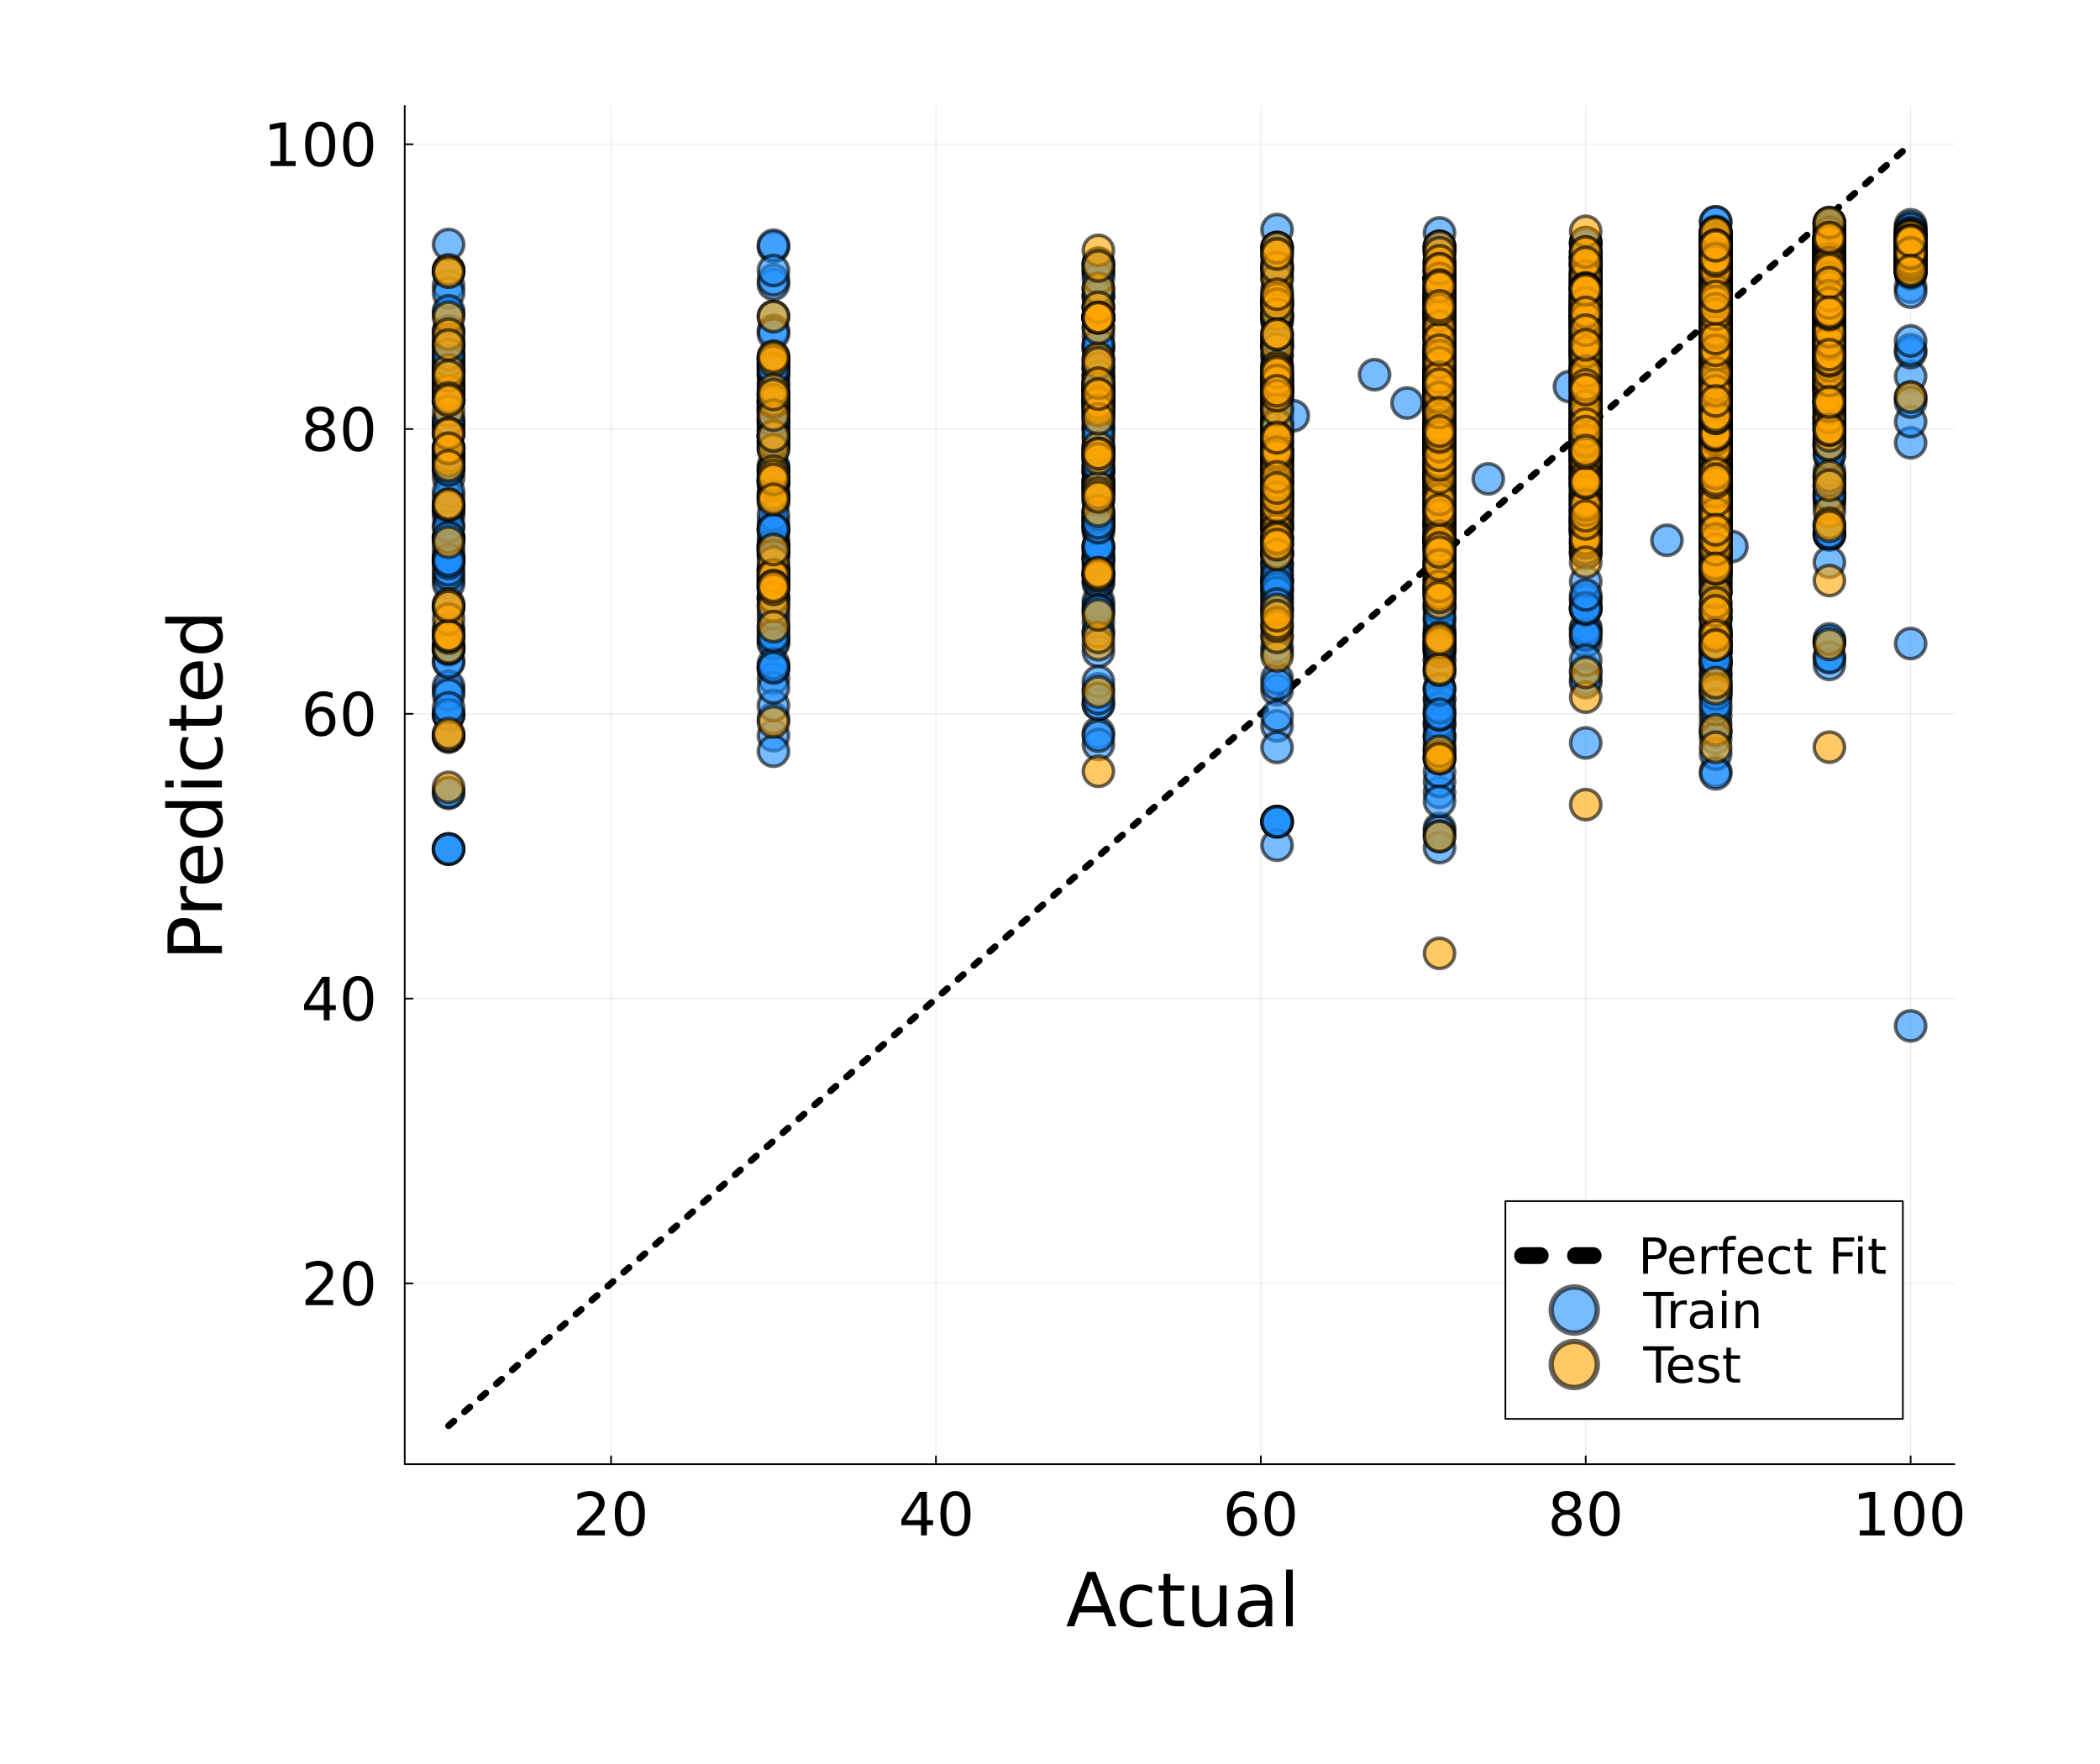
\includegraphics[width=.8\linewidth]{ols_performance.png}
\caption{Predictive Performance of the OLS Regression Model}
\label{fig:ols_performance}
\end{figure}

\FloatBarrier

Next, a logistic regression model was constructed to predict boiler maintenance classification. The logistic function, or sigmoid function, was applied to the linear predictor to estimate the probability of one class over another~\cite{brunton2022data}. An $L_2$ norm regularization term was included, like the Ridge regression model above~\cite{mlj_linear_models}. The classifications are defined using the decision threshold where a predicted likely score at or above 85 is classified as DoNothing and scores less than 85 are classified as NeedsAction.

Binary cross-entropy (BCE), also known as log loss, was used as the performance metric:
\[
\mathrm{BCE}=-\frac{1}{N}\sum_{n=1}^{N}
\left[y_n\log\hat{y}_n+(1-y_n)\log(1-\hat{y}_n)\right],
\]
where $N$ is the number of observations, $\hat{y}_n$ is the predicted probability for class 1 (NeedsAction), and $y_n$ is the true class of the observation. Lower values of log loss were preferred.

The data were first randomly partitioned into training ($80\%$) and testing ($20\%$) sets, and the hyperparameter $\lambda$ was selected using five-fold cross-validation on the training dataset. A value of $\lambda=0.001833$ was selected. The tuned model was then fit using the full training dataset, and performance was evaluated using the held-out testing $20\%$ of the data.

A testing log loss and accuracy of 0.438335 and 81.099\%, respectively, were obtained (Table~\ref{tab:Logistic_performance_comparison}). A clear cutoff or separation between the two data classes was not observed in the probability separation histogram (Figure~\ref{fig:logistic_hist}).

\begin{table}[htbp]
\centering
\caption{Logistic regression performance on training and testing datasets.}
\begin{tabular}{llcc}
\hline
Model & Dataset & Log Loss & Accuracy (\%) \\
\hline
\multirow{2}{*}{Logistic Regression}
& Train & 0.434056 & 81.327 \\
& Test & 0.438335 & 81.099 \\
\hline
\end{tabular}
\label{tab:Logistic_performance_comparison}
\end{table}

\begin{figure}
\centering
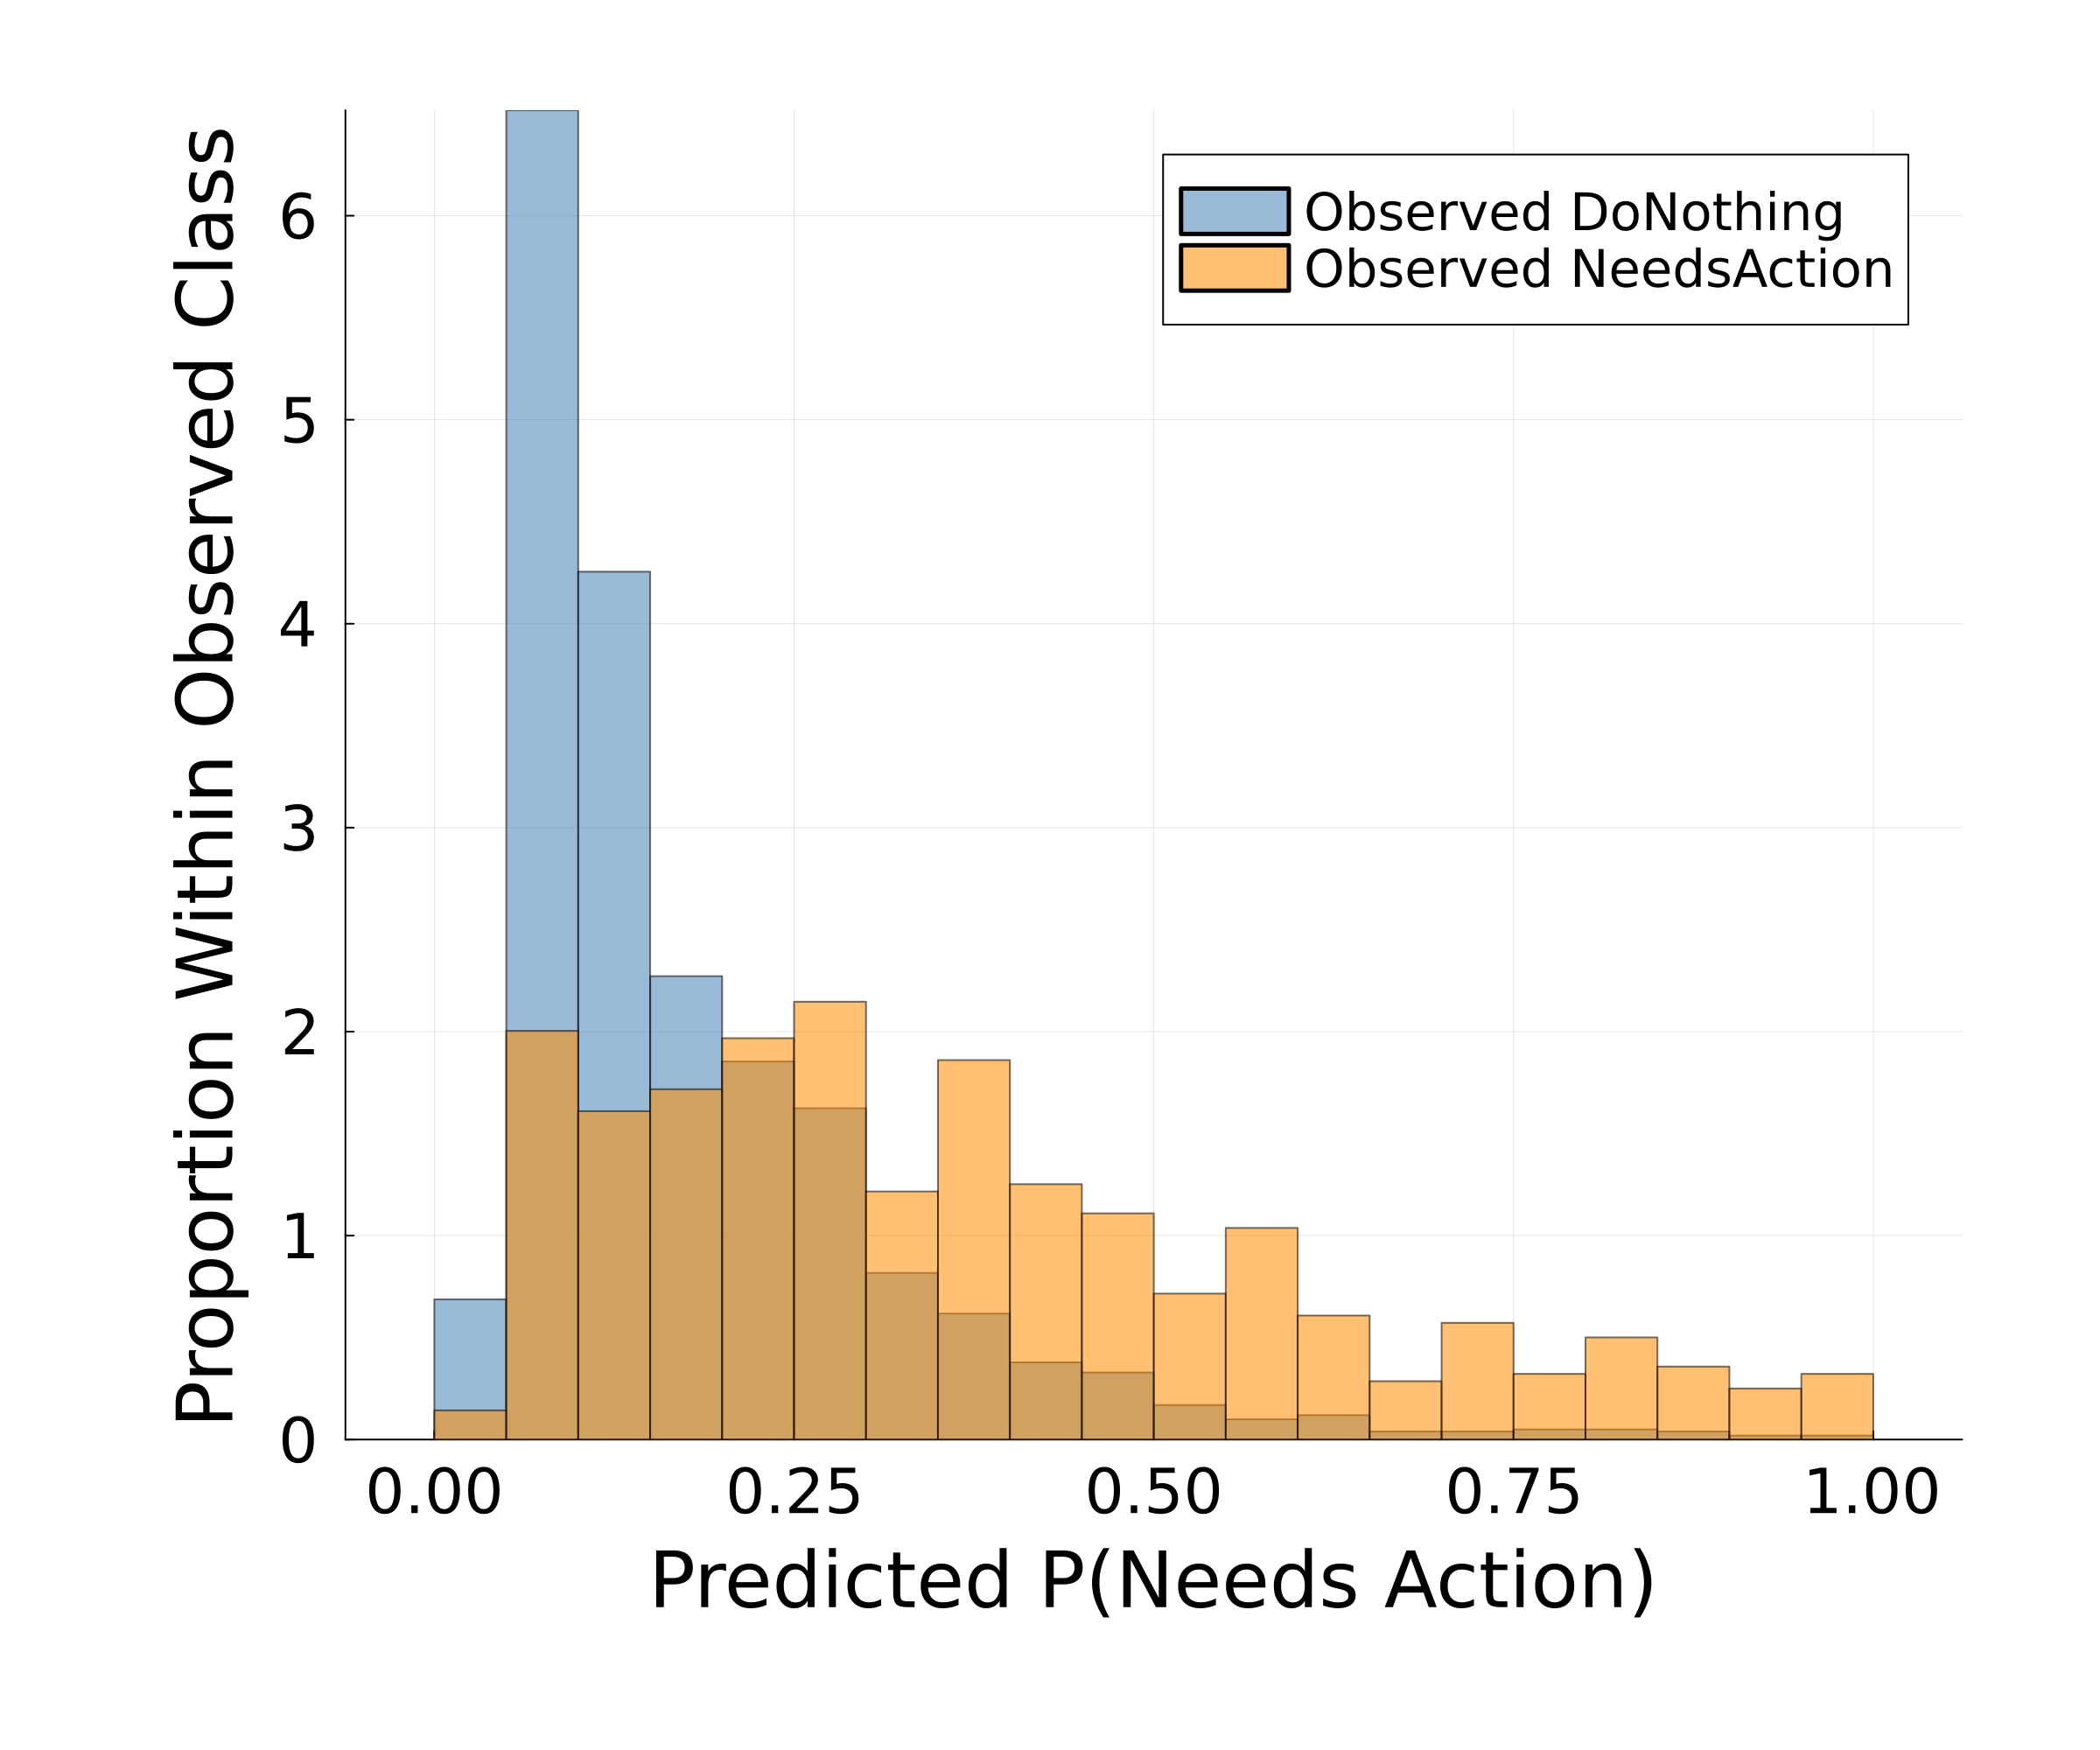
\includegraphics[width=.8\linewidth]{log_prob_sep_hist.png}
\caption{Predicted Probability by Observed Region for the Logistic Regression Model}
\label{fig:logistic_hist}
\end{figure}

\FloatBarrier

\subsection{Decision Tree}
\label{sec:dt-analysis}

A decision-tree classifier was developed using Julia's DecisionTree.jl package, with MLJBase used for data partitioning and cross-validation. The initial predictors were RSL, PredictedCI, PrevAssessed, NormalizedAssetAge, MonthSin, MonthCos, LogCRV, and Climate, selected from the earlier exploratory analysis. These variables were used directly rather than as principal-component scores. The baseline hyperparameters are shown in Table~\ref{tab:dt-baseline}.

\begin{table}[htbp]
\centering
\caption{Baseline decision-tree configuration.}
\label{tab:dt-baseline}
\small
\renewcommand{\arraystretch}{1.15}
\setlength{\tabcolsep}{5pt}
\begin{tabularx}{\linewidth}{@{}>{\raggedright\arraybackslash}X >{\raggedright\arraybackslash}p{0.36\linewidth}@{}}
\toprule
\textbf{Parameter} & \textbf{Baseline setting} \\
\midrule
Split criterion & Gini impurity \\
Feature selection & 8 predictors \\
Maximum depth & 4 \\
Minimum observations per leaf & 30 \\
Minimum observations to attempt a split & 60 \\
Training/test partition & 80\% / 20\%, stratified \\
Cross-validation & Five-fold stratified \\
NeedsAction probability cutoff & 0.50 \\
Random seed & 1234 \\
\bottomrule
\end{tabularx}
\end{table}

The data were prepared using the boiler filter and derived predictors described in the earlier Data Wrangling section. Missing PrevScore, Recency, and Climate values were replaced with means, as in the earlier analysis. For decision-tree validation, these means were calculated from the training data in each split rather than from the full dataset. Every feature set was evaluated on the same assessment records. Score was not used as a predictor; identifiers were also excluded from the inputs.

Observations were split into groups using Gini impurity. In each final group, or leaf, the NeedsAction probability was estimated from the proportion of its training observations in that category. The data were divided into approximately 80\% training and 20\% testing using a stratified split and random seed 1234. Five-fold cross-validation (CV) was performed on the training data, with the same folds used for all experiments and replacement means recalculated within each fold. Log loss was used to evaluate the predicted probabilities. It was calculated using natural logarithms and numerical clipping to avoid $\log(0)$.

Maximum depths of 2, 3, 4, 5, 6, and 8 were tested with minimum leaf sizes of 10, 30, and 60. All 18 depth--leaf combinations were evaluated for each of ten feature sets, giving 180 configurations. The minimum number of observations required to attempt a split was set to twice the minimum leaf size.

The feature sets before and after tuning are compared in Table~\ref{tab:dt-features}. The original eight predictors were included in Baseline8. For the ``No'' configurations, the named predictor was removed, with PredictedCI removed for NoCI7 and both month variables removed for NoSeason6. PrevScore and Recency were added for History10, NormalizedAge and EffectiveAge for Lifecycle10, and all four for Expanded12. Maximum depth 4 and minimum leaf size 30 were used for the fixed-setting results.

\begin{table}[htbp]
\centering
\caption{Decision-tree feature selection and tuning results.}
\label{tab:dt-features}
\small
\renewcommand{\arraystretch}{1.15}
\setlength{\tabcolsep}{4pt}
\begin{tabularx}{\linewidth}{@{}>{\raggedright\arraybackslash}X c r r c c@{}}
\toprule
\textbf{Feature set} &
\textbf{Inputs} &
\shortstack{\textbf{Fixed CV}\\\textbf{log loss}} &
\shortstack{\textbf{Tuned CV}\\\textbf{log loss}} &
\shortstack{\textbf{Best}\\\textbf{depth}} &
\shortstack{\textbf{Best leaf}\\\textbf{minimum}} \\
\midrule
Baseline8       & 8  & 0.408122 & 0.401183 & 5 & 60 \\
NoRSL7          & 7  & 0.418974 & 0.417440 & 5 & 60 \\
NoCI7           & 7  & 0.405361 & 0.398774 & 5 & 60 \\
NoSeason6       & 6  & 0.407231 & 0.403239 & 5 & 60 \\
NoClimate7      & 7  & 0.413878 & 0.412898 & 5 & 60 \\
NoPrevAssessed7 & 7  & 0.407790 & 0.401652 & 5 & 60 \\
NoMonthCos7     & 7  & 0.406208 & 0.402895 & 5 & 60 \\
History10       & 10 & 0.410055 & 0.401831 & 5 & 60 \\
Lifecycle10     & 10 & 0.406503 & 0.401480 & 5 & 60 \\
Expanded12      & 12 & 0.407465 & 0.401991 & 5 & 60 \\
\bottomrule
\end{tabularx}
\end{table}

The best result was obtained with NoCI7, maximum depth 5, and minimum leaf size 60. Its CV log loss of 0.398774 was approximately 2.29\% lower than the fixed baseline. The same depth--leaf combination was selected for every feature set; minimum leaf sizes above 60 were not evaluated. The test data were not used to select the model. Tuning results for the original eight predictors are shown in Figure~\ref{fig:dt-hyperparameters}.

\begin{figure}[htbp]
\centering
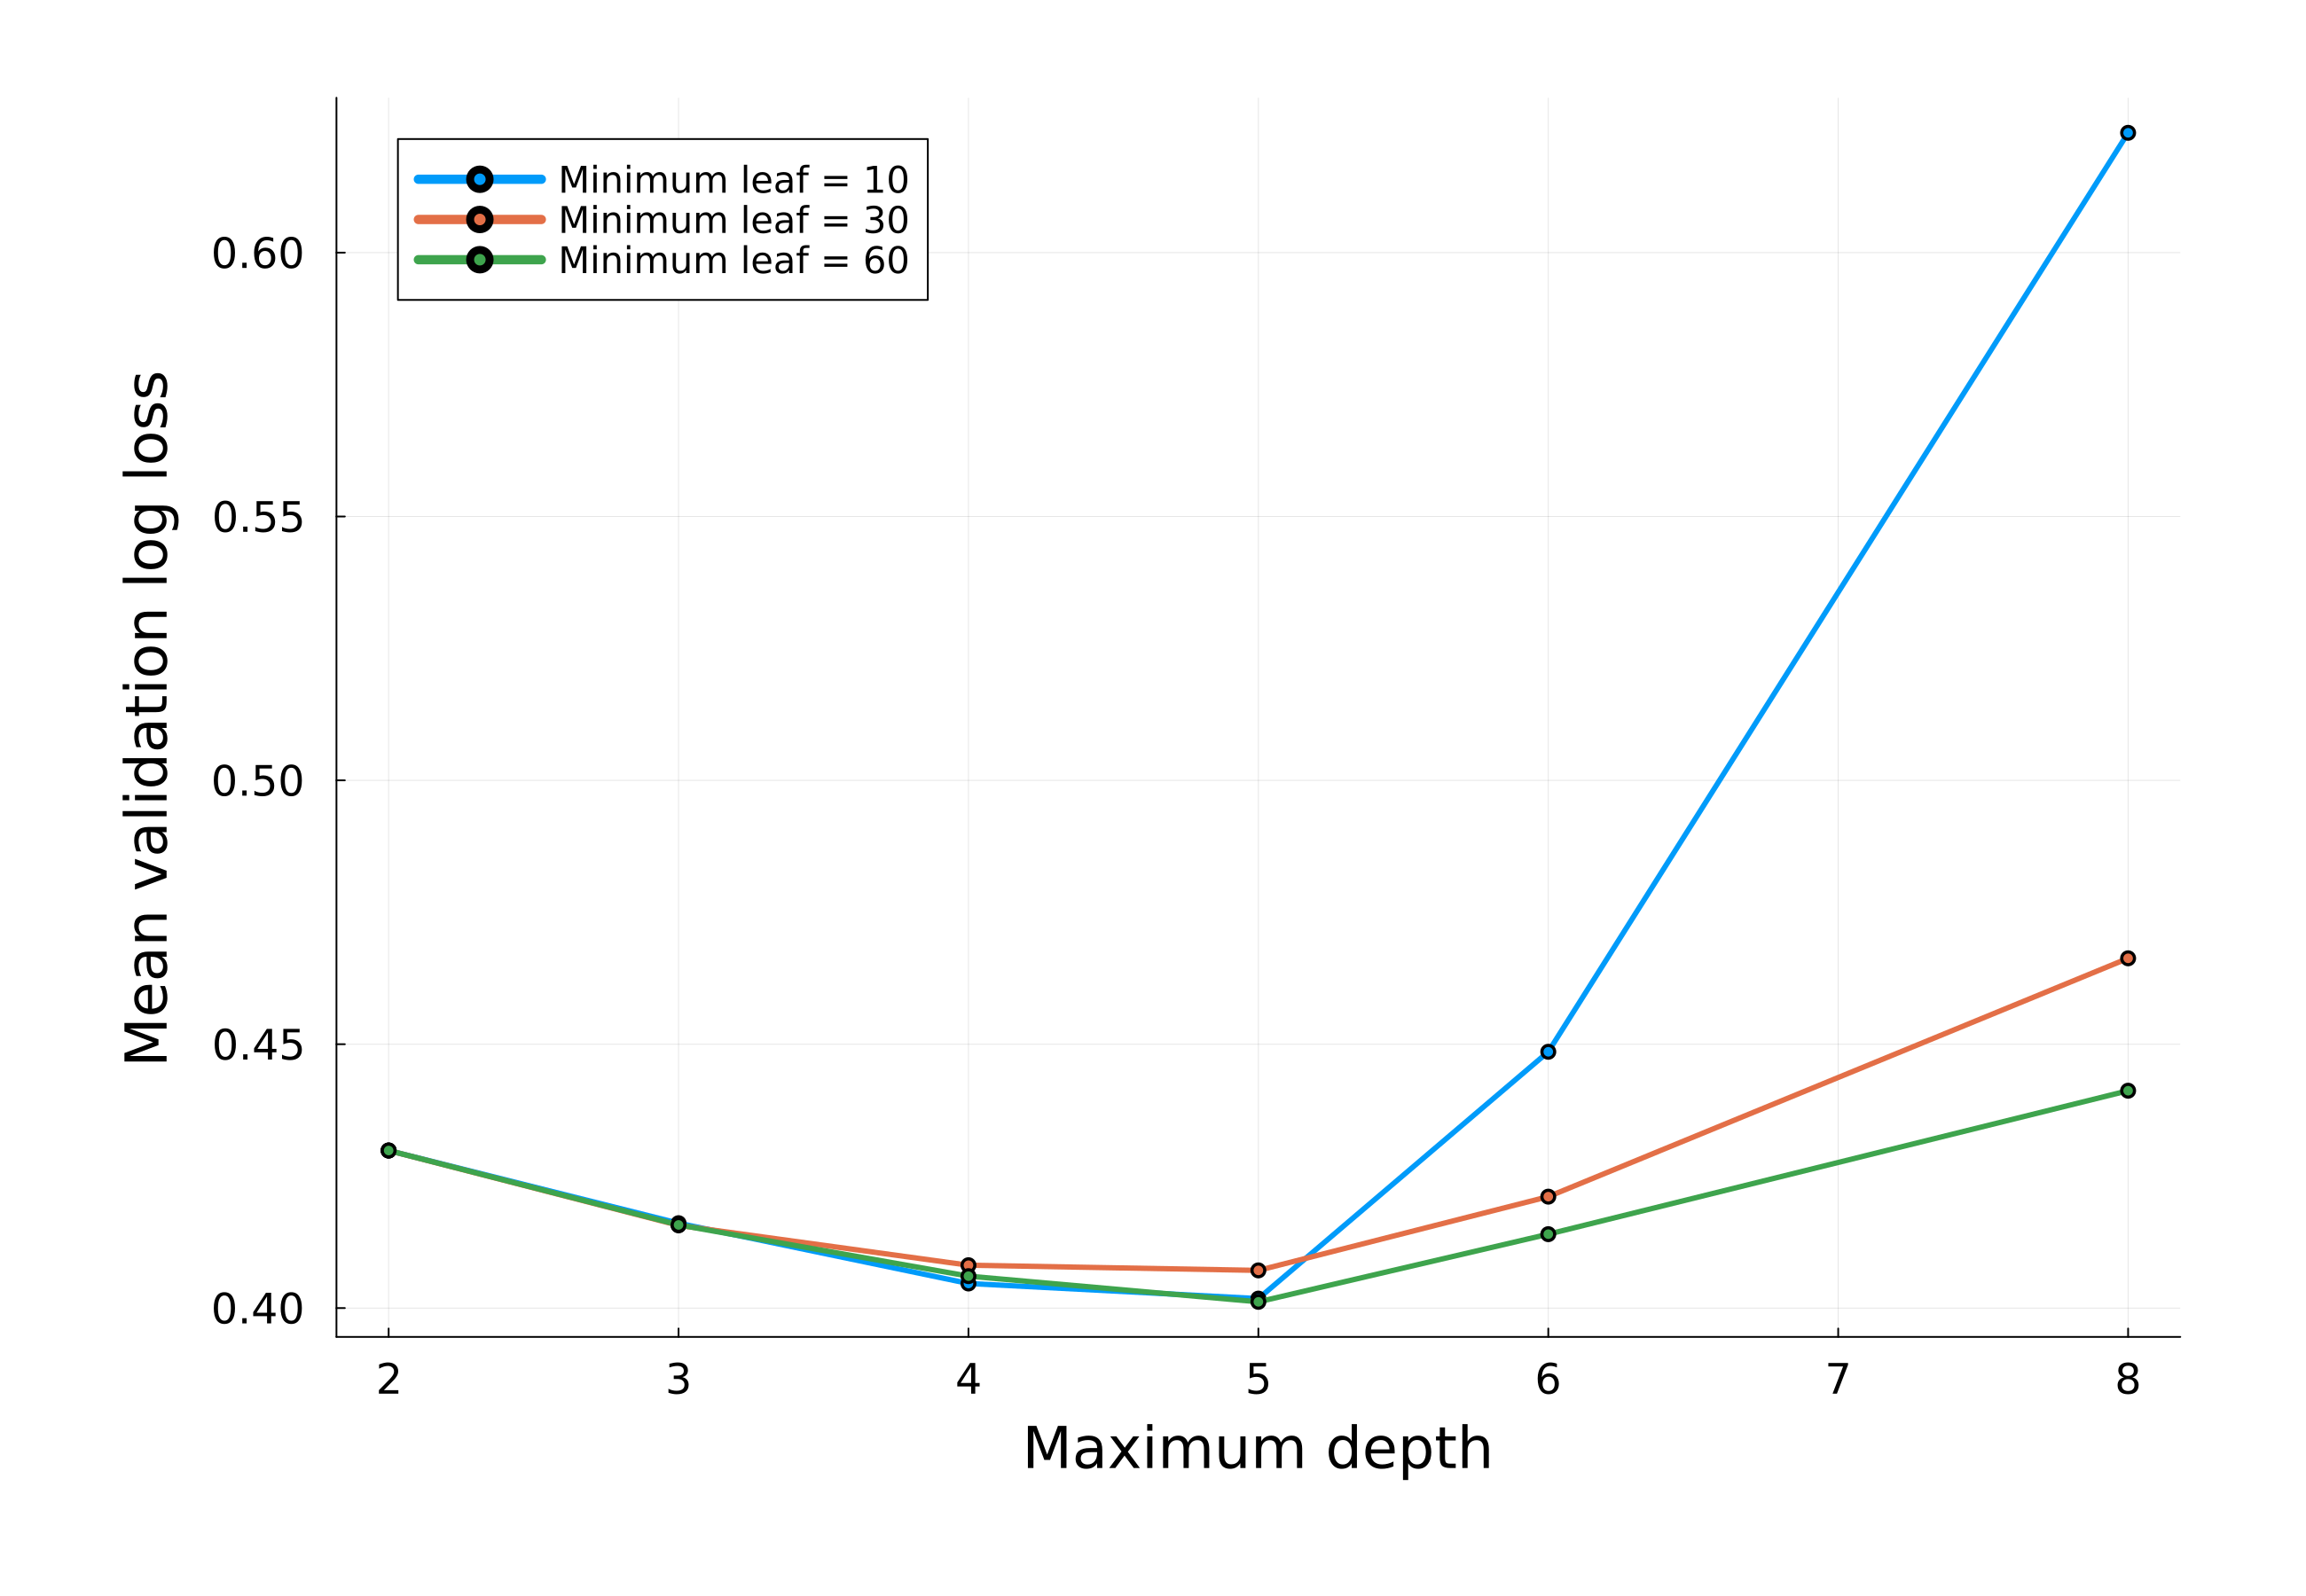
\includegraphics[width=.8\linewidth]{DT_Hyperparameter_Optimization.png}
\caption{Decision Tree Tuning}
\label{fig:dt-hyperparameters}
\end{figure}

The baseline and selected tree were refitted on all training observations and evaluated on the same test subset (Table~\ref{tab:dt-performance}). Test log loss was reduced from 0.415814 to 0.413995, approximately 0.44\%. The improvement was smaller than that observed during cross-validation, and its statistical significance has not been established. At the 0.50 cutoff, recall was increased from 32.97\% to 36.38\%, and F1 from 45.60\% to 47.65\%, while accuracy and precision were reduced. NeedsAction was treated as the positive class, and the classification metrics in the table are expressed as percentages.

\begin{table}[htbp]
\centering
\caption{Decision-tree performance on the held-out test subset.}
\label{tab:dt-performance}
\small
\renewcommand{\arraystretch}{1.15}
\setlength{\tabcolsep}{8pt}
\begin{tabularx}{0.85\linewidth}{@{}>{\raggedright\arraybackslash}X r r@{}}
\toprule
\textbf{Metric} & \textbf{Baseline tree} & \textbf{Selected tree} \\
\midrule
Log loss       & 0.415814 & 0.413995 \\
Accuracy (\%)  & 82.89    & 82.62    \\
Precision (\%) & 73.90    & 69.05    \\
Recall (\%)    & 32.97    & 36.38    \\
F1 (\%)        & 45.60    & 47.65    \\
\bottomrule
\end{tabularx}
\end{table}

The selected tree's test confusion matrix is shown in Figure~\ref{fig:dt-confusion}, with predicted categories on rows and observed categories on columns. Nearly two-thirds of the actual NeedsAction assessments were missed at the 0.50 cutoff, despite most test observations being classified correctly overall.

\begin{figure}[htbp]
\centering
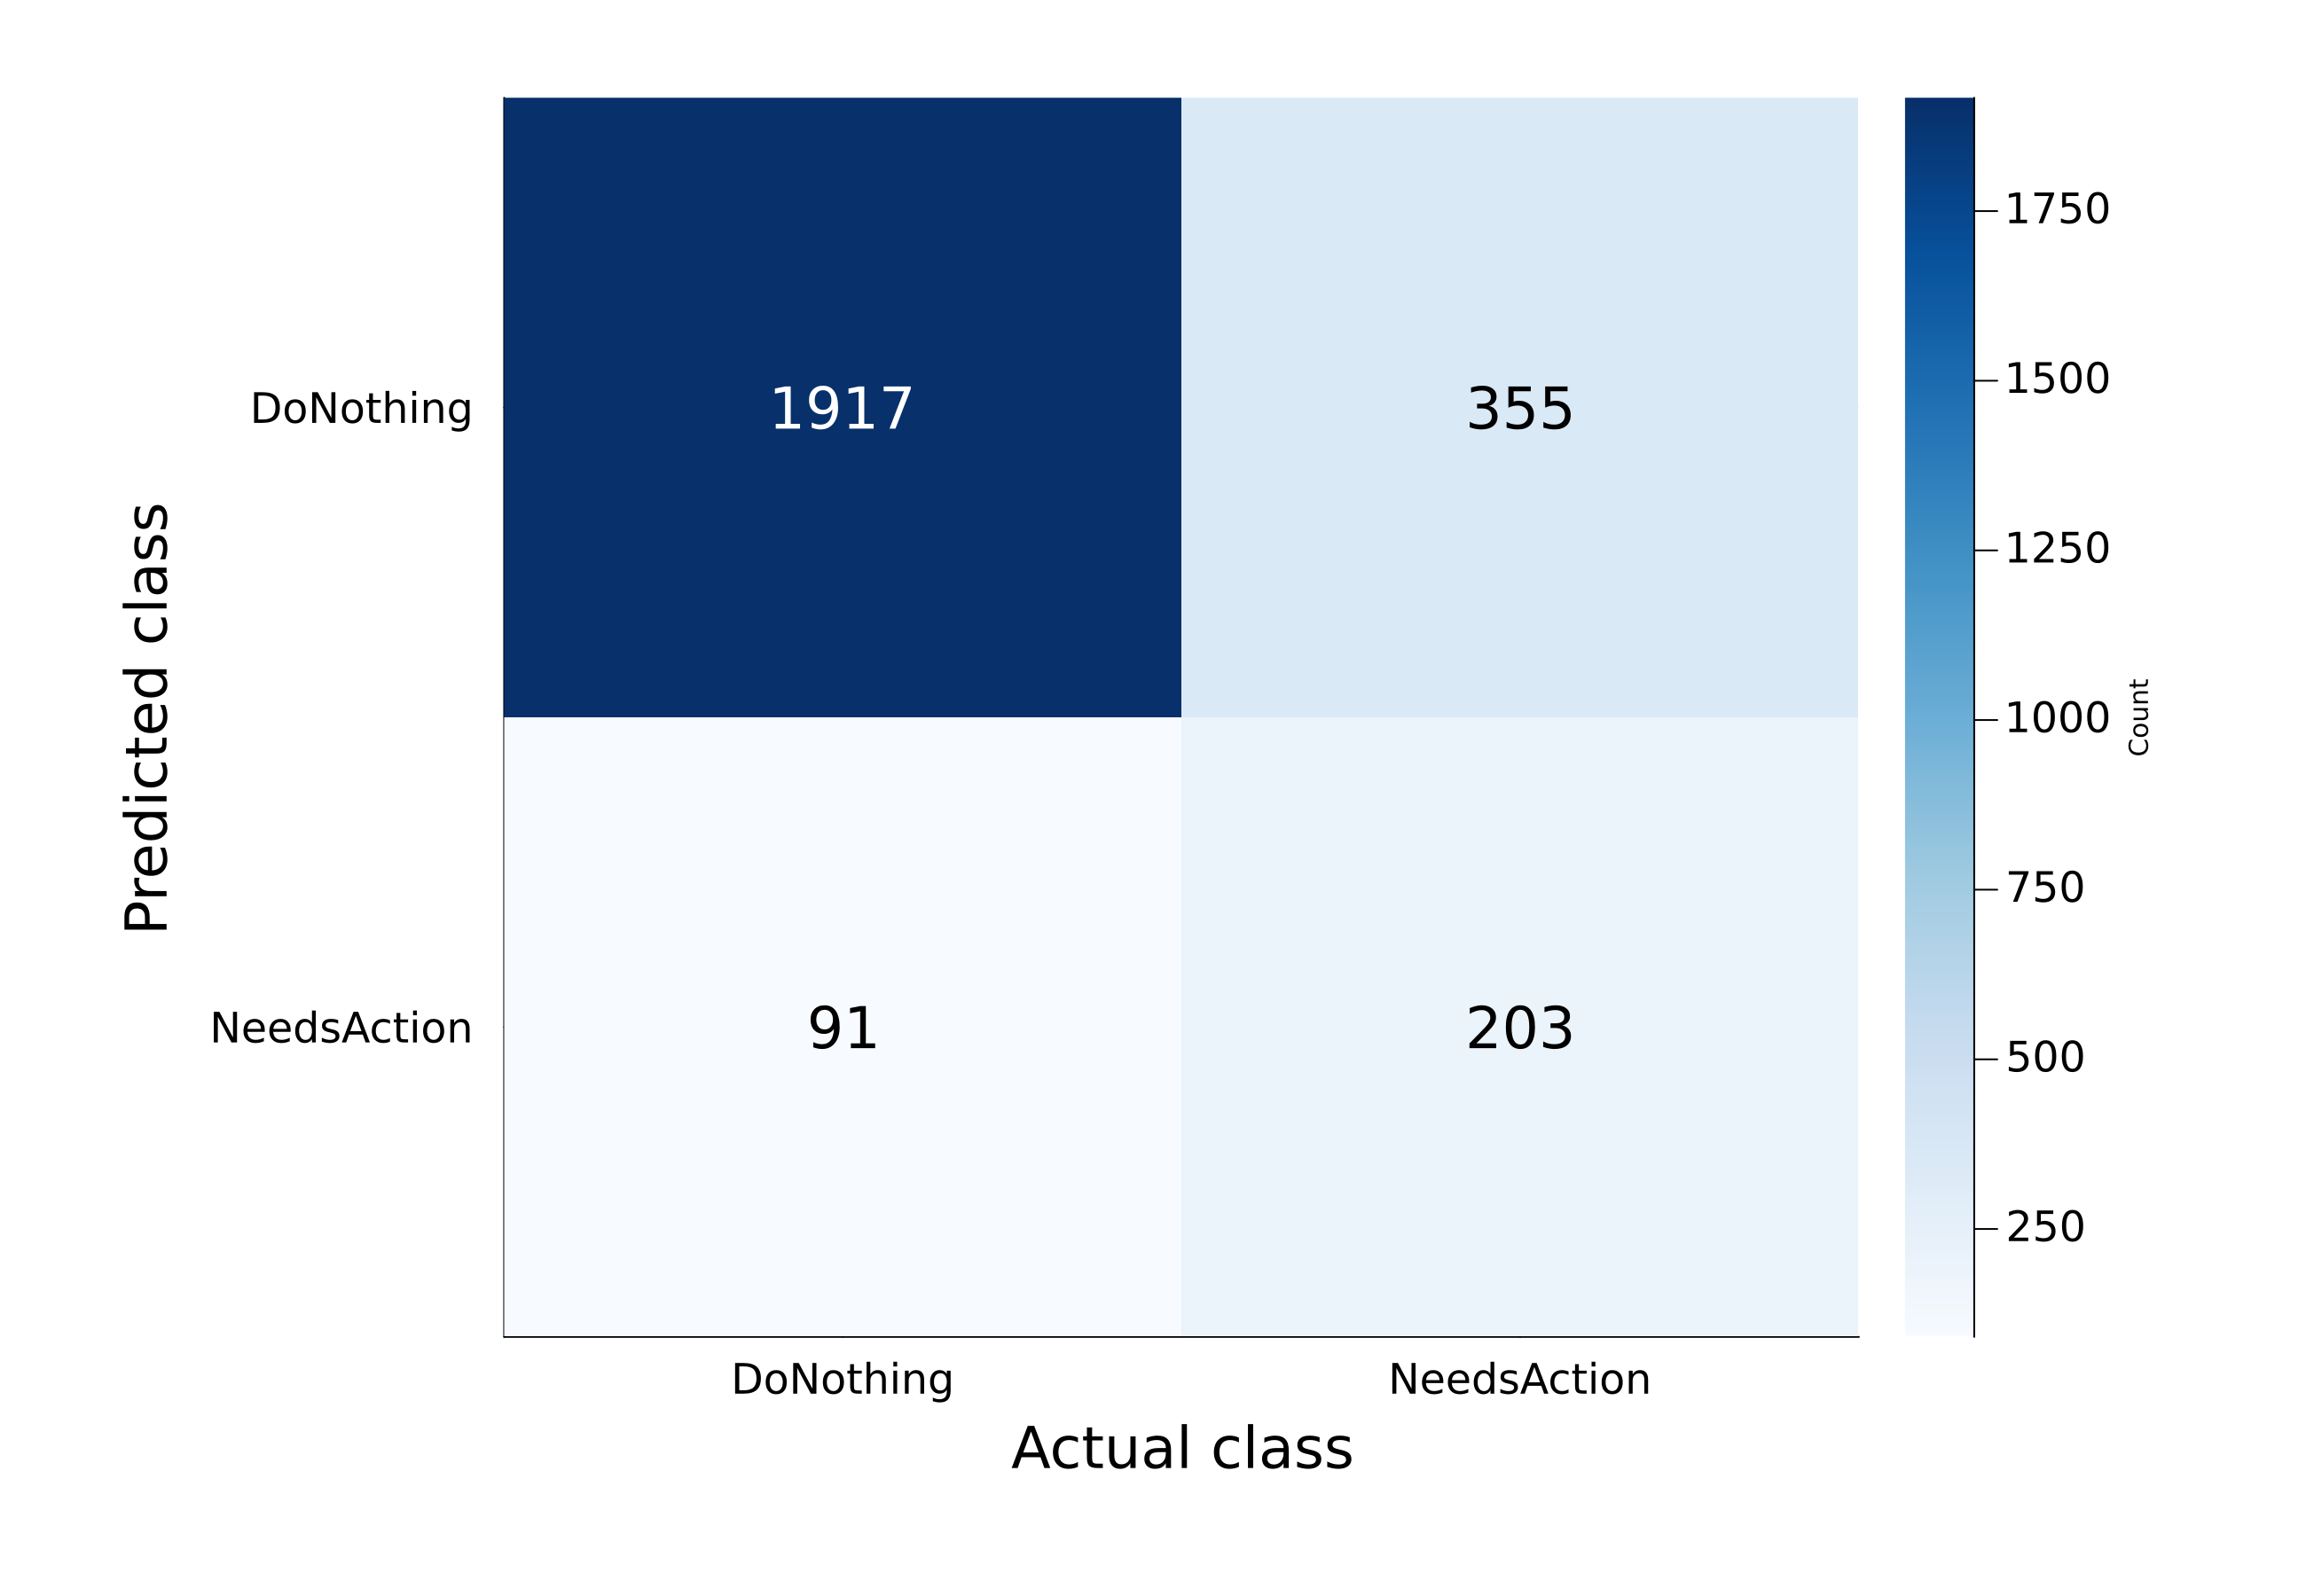
\includegraphics[width=.8\linewidth]{DT_Confusion_Matrix.png}
\caption{Decision Tree Confusion Matrix}
\label{fig:dt-confusion}
\end{figure}

The largest normalized Gini importance was assigned to RSL at 0.7790, followed by Climate at 0.1082 and PrevAssessed at 0.0498 (Figure~\ref{fig:dt-importance}). LogCRV was retained in the input set but was assigned zero importance in the fitted tree. The prominence of RSL and Climate was consistent with the higher validation losses when these variables were removed. The importance values were based on reductions in training impurity; causal effects or a predictor's usefulness in other models cannot be established from them.

\begin{figure}[htbp]
\centering
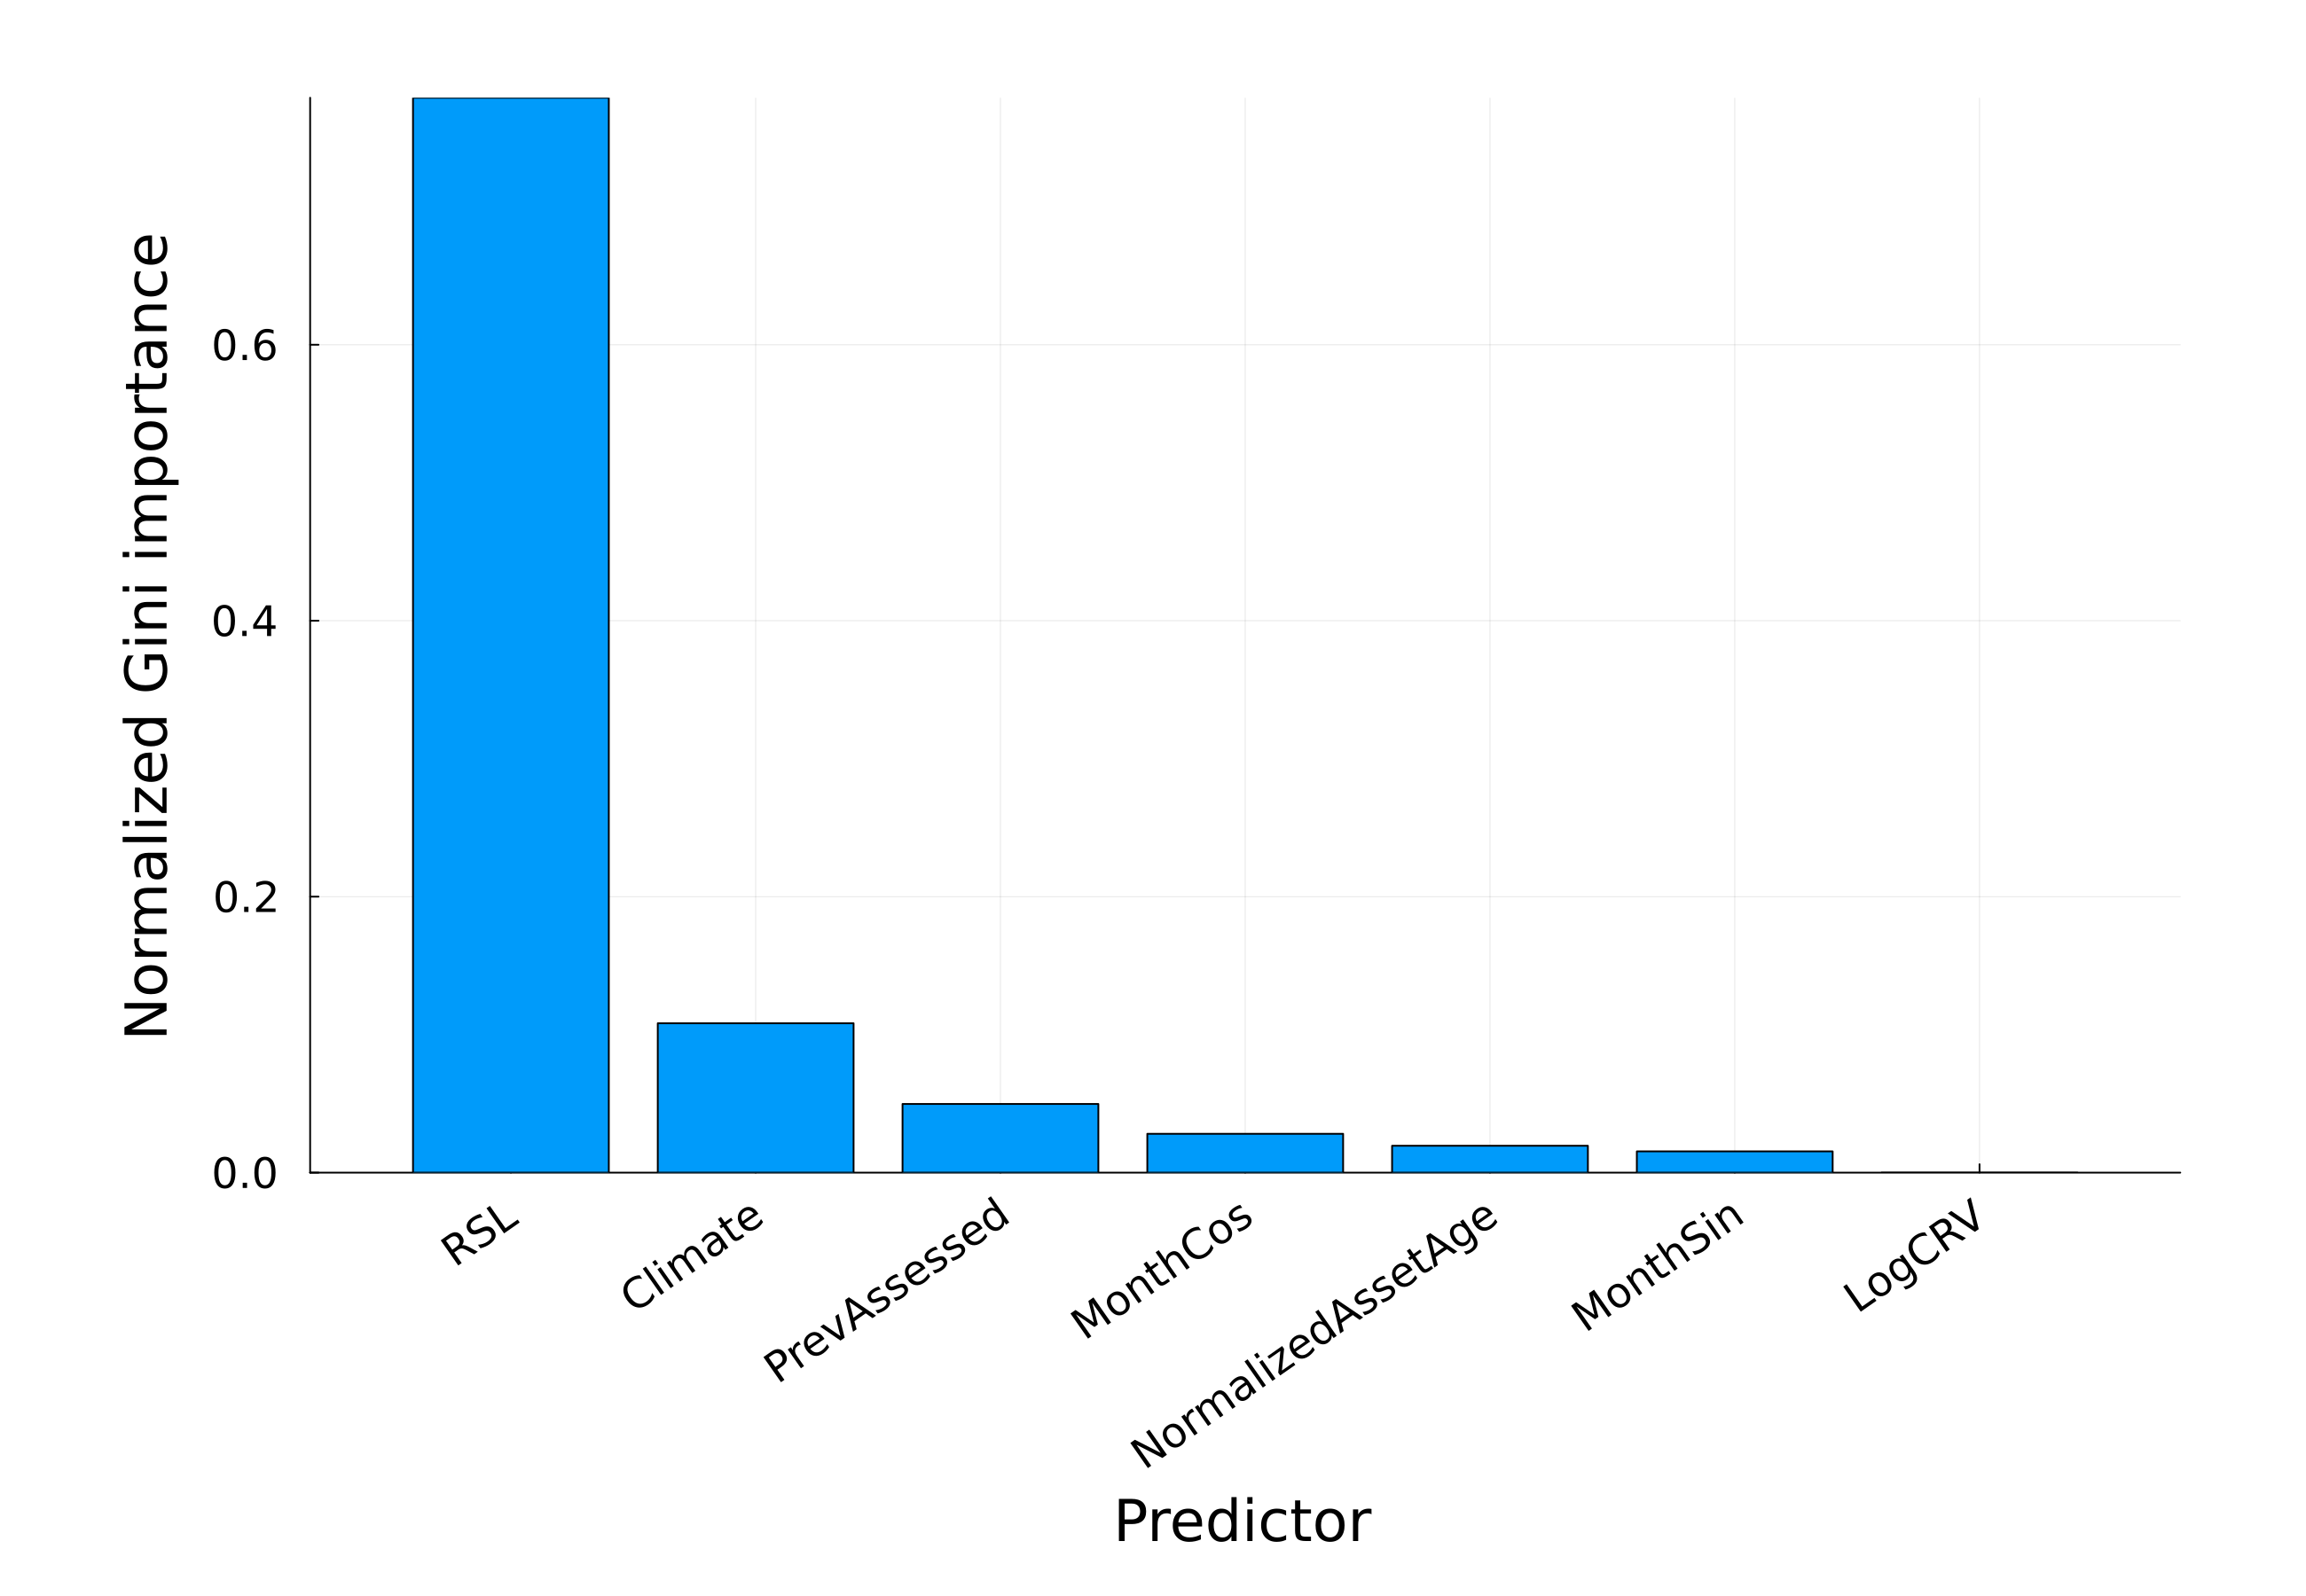
\includegraphics[width=.8\linewidth]{DT_Feature_Importance.png}
\caption{Decision Tree Predictor Importance}
\label{fig:dt-importance}
\end{figure}

Evaluation was performed using a random split of assessment records rather than a split by component or assessment date, so performance on new components and future assessments has not been verified. Predictor availability before a new assessment and the numerical treatment of Climate should also be considered for practical use.

\FloatBarrier

\subsection{Artificial Neural Network (ANN)}

An artificial neural network (ANN) was developed using Julia's MLJ, Flux, and Optimisers packages. The ANN was configured to be a binary classifier for deriving decision region probabilities in a value of information model. The same eight predictors used for the regression and baseline decision-tree models were included in the initial feature set. Baseline hyperparameters are shown in Table~\ref{tab:ann-baseline}.

\begin{table}[htbp]
\centering
\caption{Baseline ANN configuration.}
\label{tab:ann-baseline}
\begin{tabular}{ll}
\hline
\textbf{Parameter} & \textbf{Baseline setting} \\
\hline
ANN architecture & Two hidden layers: 16 and 8 nodes \\
Learning Rate & 0.001 \\
Regularization & $\lambda = 0.0001$ \\
Feature selection & 8 predictors \\
Epochs & 150 \\
Batch size & 32 \\
Optimizer & Adam \\
\hline
\end{tabular}
\end{table}

Cross-validation was performed with a five-fold strategy on 80\% of the total data, with 20\% held out for testing. A cross-validation log loss of approximately 0.3986 and held-out test log loss of approximately 0.4014 were obtained for the baseline ANN (Table~\ref{tab:ann-baseline-performance}). In a prevalence only model, the same probability distribution is assigned to every observation based on the observed frequency in the training data ($\approx$ 79\% DoNothing, 21\% NeedsAction). The prevalence only log loss of 0.5237 is used as a baseline for comparison against the 0.4014 for the baseline ANN. The relative reduction is approximately 23.4\%. At the 0.50 cutoff, approximately 40\% of all observed NeedsAction cases were identified by the baseline ANN.

\begin{table}[htbp]
\centering
\caption{Performance of the initial baseline ANN using the held-out test subset. Precision, recall, and accuracy are expressed as proportions.}
\label{tab:ann-baseline-performance}
\begin{tabular}{lr}
\hline
\textbf{Metric} & \textbf{Value} \\
\hline
Cross-validated log loss & 0.398558 \\
Held out test log loss & 0.401356 \\
Prevalence only baseline test log loss & 0.523673 \\
Relative reduction in test log loss & 23.4\% \\
Precision at 0.50 cutoff & 0.713376 \\
Recall at 0.50 cutoff & 0.401434 \\
Accuracy at 0.50 cutoff & 0.834762 \\
\hline
\end{tabular}
\end{table}

With the baseline developed, a series of experiments were performed to improve upon the initial hyperparameter selection. Iterative tests were performed by sweeping different values of one parameter at a time, with the best settings retained for successive tests (Table~\ref{tab:ann-tuning}). Baseline epochs, batch size, optimizer, and learning rate were retained, while $\lambda$ and hidden layer configuration parameters were updated. Forty architecture selections were tried, with one hidden layer of 112 nodes selected. Randomization was initialized with a fixed seed to ensure experimentation was repeatable.

With hyperparameters tuned, the final stage of experimentation was variable feature selection. Trials of approximately 100 feature combinations were performed, and RSL, NormalizedAge, EffectiveAge, PredictedCI, Recency, PrevScore, PrevAssessed, NormalizedAssetAge, MonthSin, MonthCos, LogCRV, and Climate were selected. While the performance difference was minimal, lower log loss was obtained with the inclusion of additional lifecycle parameters. The selected ANN configuration is shown in Table~\ref{tab:ann-configuration}.

\begin{table}[htbp]
\centering
\caption{Summary of ANN tuning experiments.}
\label{tab:ann-tuning}
\begin{tabular}{llll}
\hline
\textbf{Experiment} & \textbf{Configurations} & \textbf{Selected setting} & \textbf{Best CV log loss} \\
\hline
Network architecture & 40 architectures & One 112 node layer & 0.384918 \\
Learning rate & 9 values & 0.001 & 0.384918 \\
Regularization & 12 $\lambda$ values & $\lambda = 0.01$ & 0.383320 \\
Feature selection & 100 combinations & 12 features & 0.377854 \\
Epochs & 12 values & 150 & No Improvement \\
Batch size & 12 values & 32 & No Improvement \\
Optimizer & 10 models & Adam & No Improvement \\
PCA Space & 1-6 PC modes & None & No Improvement \\
\hline
\end{tabular}
\end{table}

\begin{table}[htbp]
\centering
\caption{Selected ANN configuration.}
\label{tab:ann-configuration}
\begin{tabular}{ll}
\hline
\textbf{Model element} & \textbf{Selected setting} \\
\hline
Input representation & Standardized parameters; no PCA \\
Selected feature count & 12 \\
Hidden-layer architecture & One hidden layer with 112 nodes \\
Optimizer & Adam \\
Learning rate & 0.001 \\
Regularization coefficient ($\lambda$) & 0.01 \\
Epochs & 150 \\
Batch size & 32 \\
Train/test partition & 80\% / 20\%, stratified \\
Cross-validation & Five-fold stratified cross-validation \\
\hline
\end{tabular}
\end{table}

Held-out test log loss was reduced from 0.4014 to 0.3885, and the relative reduction from the prevalence-only baseline was increased from 23.4\% to 25.8\% (Table~\ref{tab:ann-performance}). At the 0.50 cutoff, precision was increased from 0.713376 to 0.726644, while recall was reduced from 0.401434 to 0.376344 and accuracy from 0.834762 to 0.833593. A smaller proportion of actual NeedsAction cases was therefore identified despite the lower log loss.

\begin{table}[htbp]
\centering
\caption{Performance of the selected ANN using the held-out test subset. Precision, recall, and accuracy are expressed as proportions.}
\label{tab:ann-performance}
\begin{tabular}{lr}
\hline
\textbf{Metric} & \textbf{Value} \\
\hline
Cross-validated log loss & 0.377854 \\
Held-out test log loss & 0.388509 \\
Prevalence-only baseline test log loss & 0.523673 \\
Relative reduction in test log loss & 25.8\% \\
Precision at 0.50 cutoff & 0.726644 \\
Recall at 0.50 cutoff & 0.376344 \\
Accuracy at 0.50 cutoff & 0.833593 \\
\hline
\end{tabular}
\end{table}

A threshold selection tradeoff was examined for cutoffs between 0.2 and 0.9 (Figure~\ref{fig:ann_cutoff_tradeoff}); reasonable selections could vary between .3 and .5 depending on decision maker priority. For boilers observed in DoNothing, predominantly low $P(\mathrm{NeedsAction})$ values were assigned; however, more evenly distributed probabilities were assigned to boilers observed in NeedsAction, with a slight bias toward low probabilities (Figure~\ref{fig:ann_probs_by_region}). A clear distinction between the two categories was not obtained.

\begin{figure}
\centering
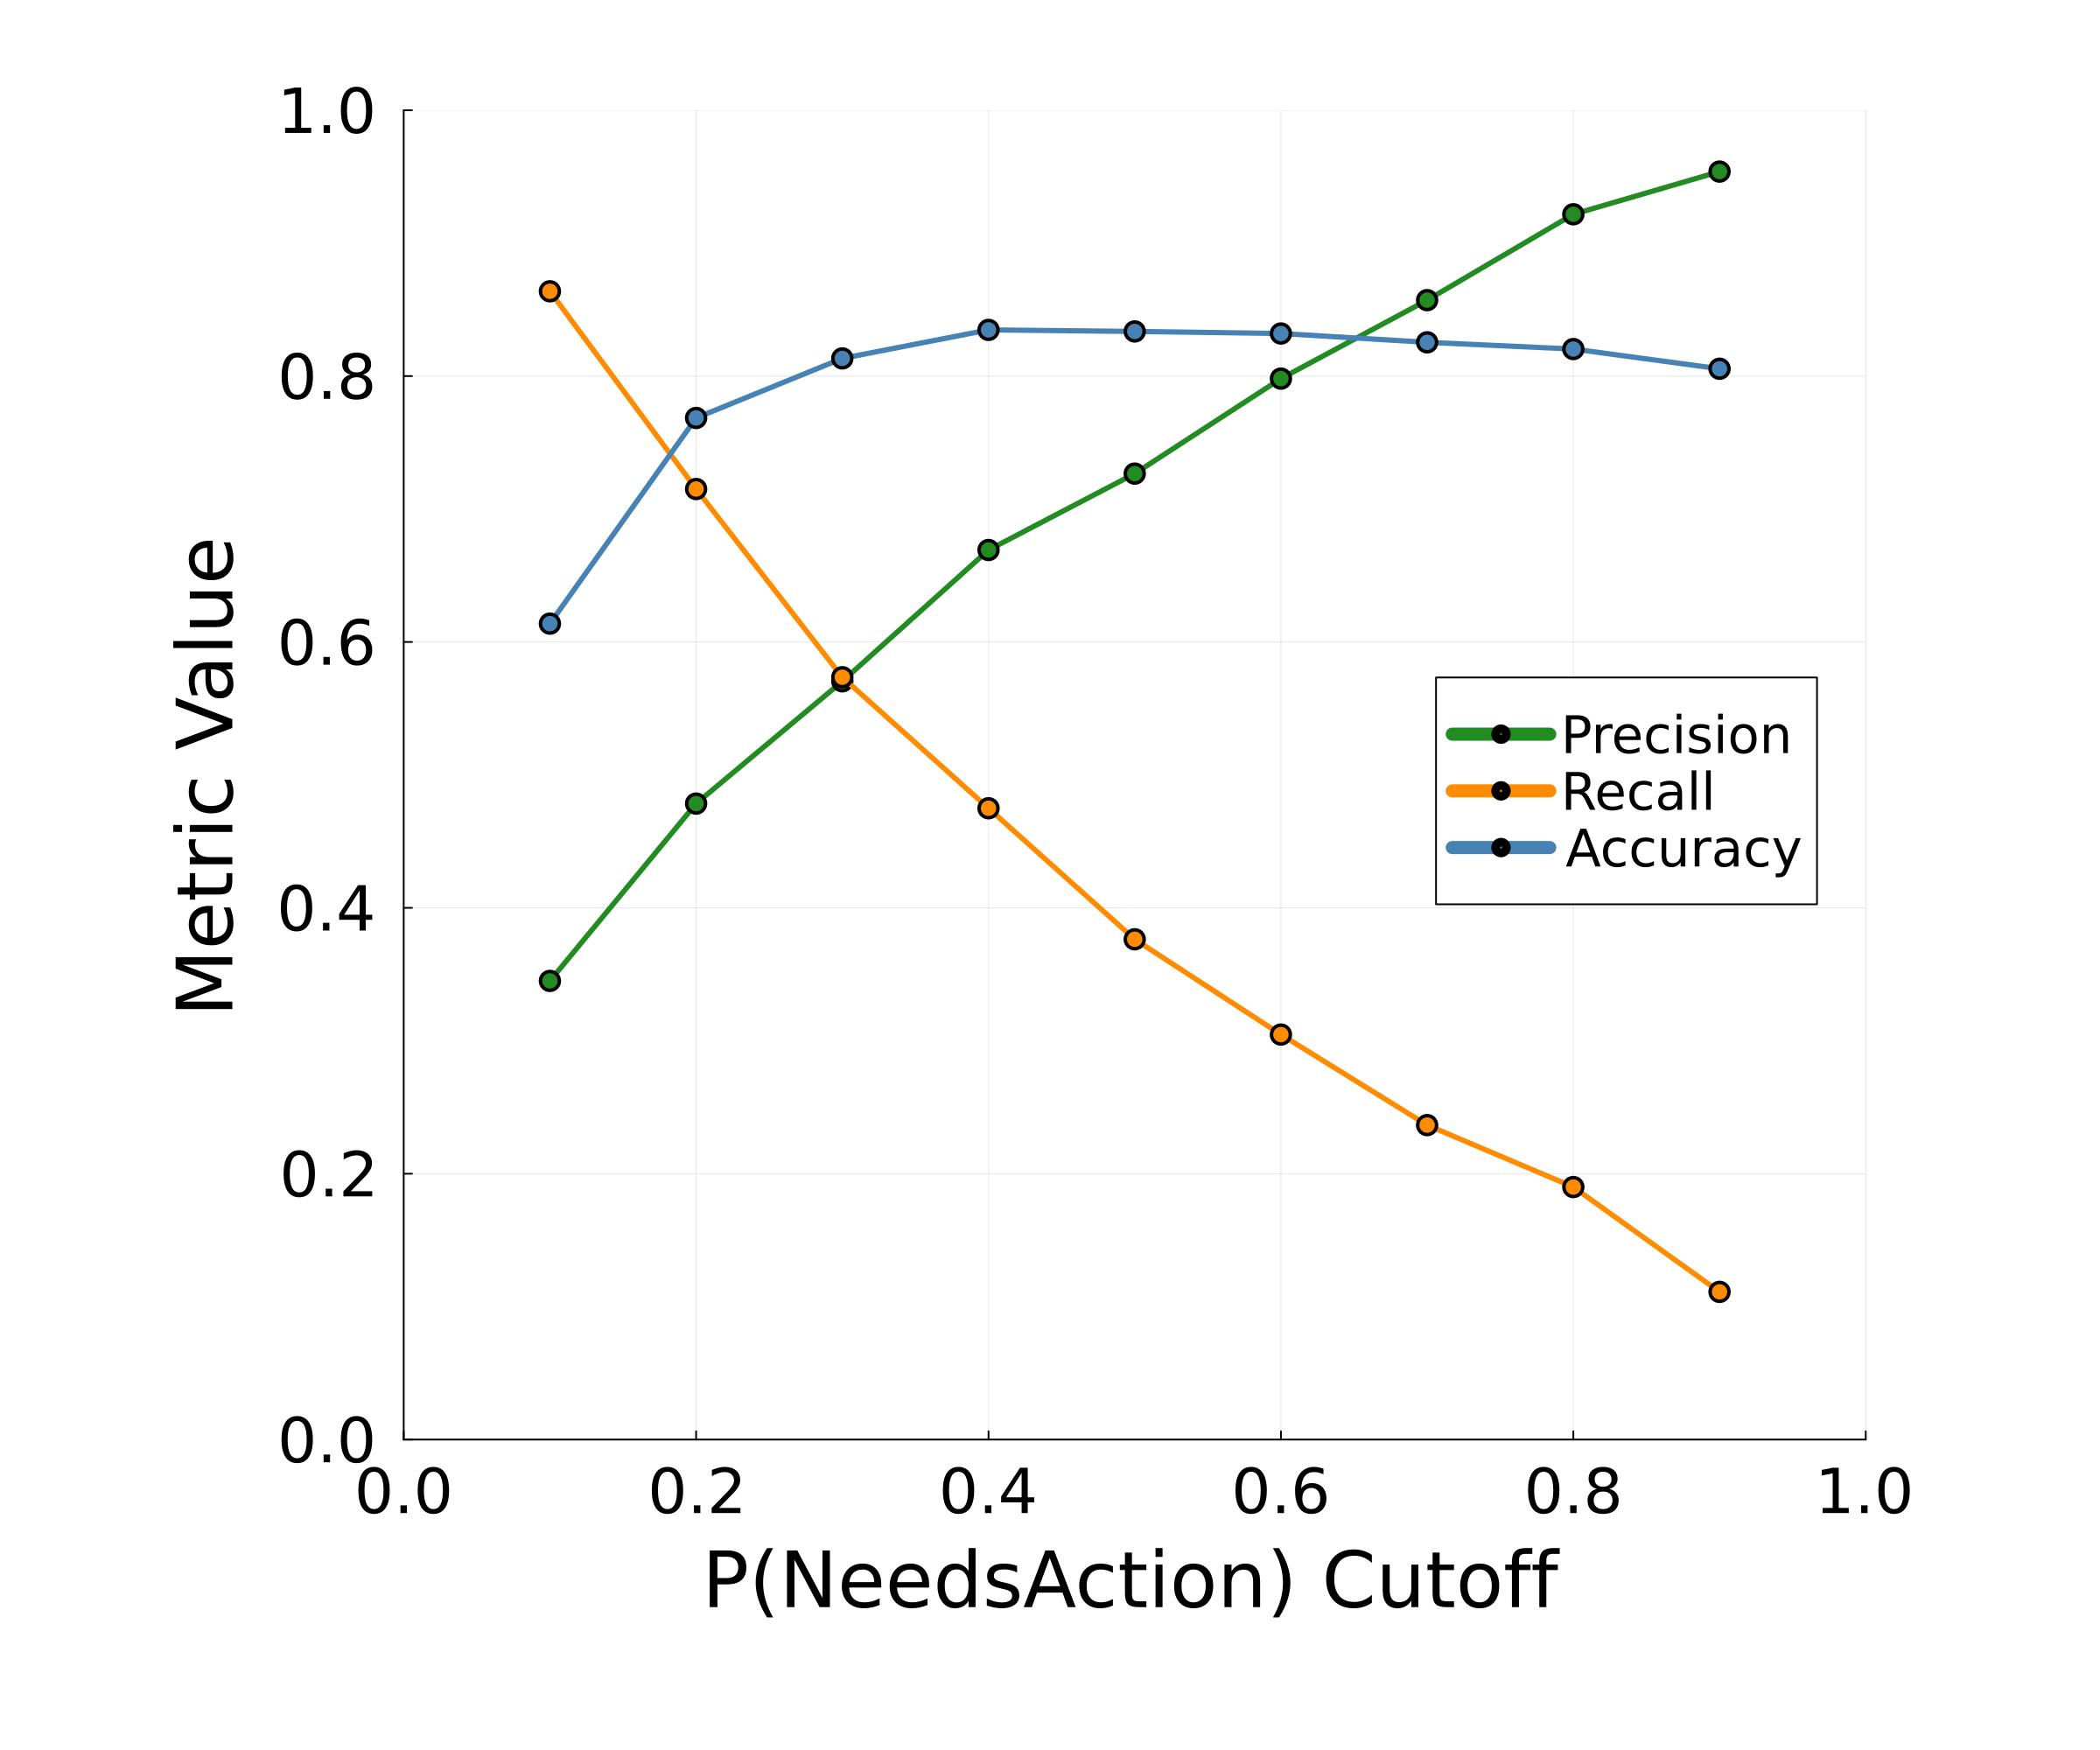
\includegraphics[width=.8\linewidth]{ANN_Cutoff_Tradeoff.png}
\caption{Classifier Threshold Selection Tradeoff}
\label{fig:ann_cutoff_tradeoff}
\end{figure}

\begin{figure}
\centering
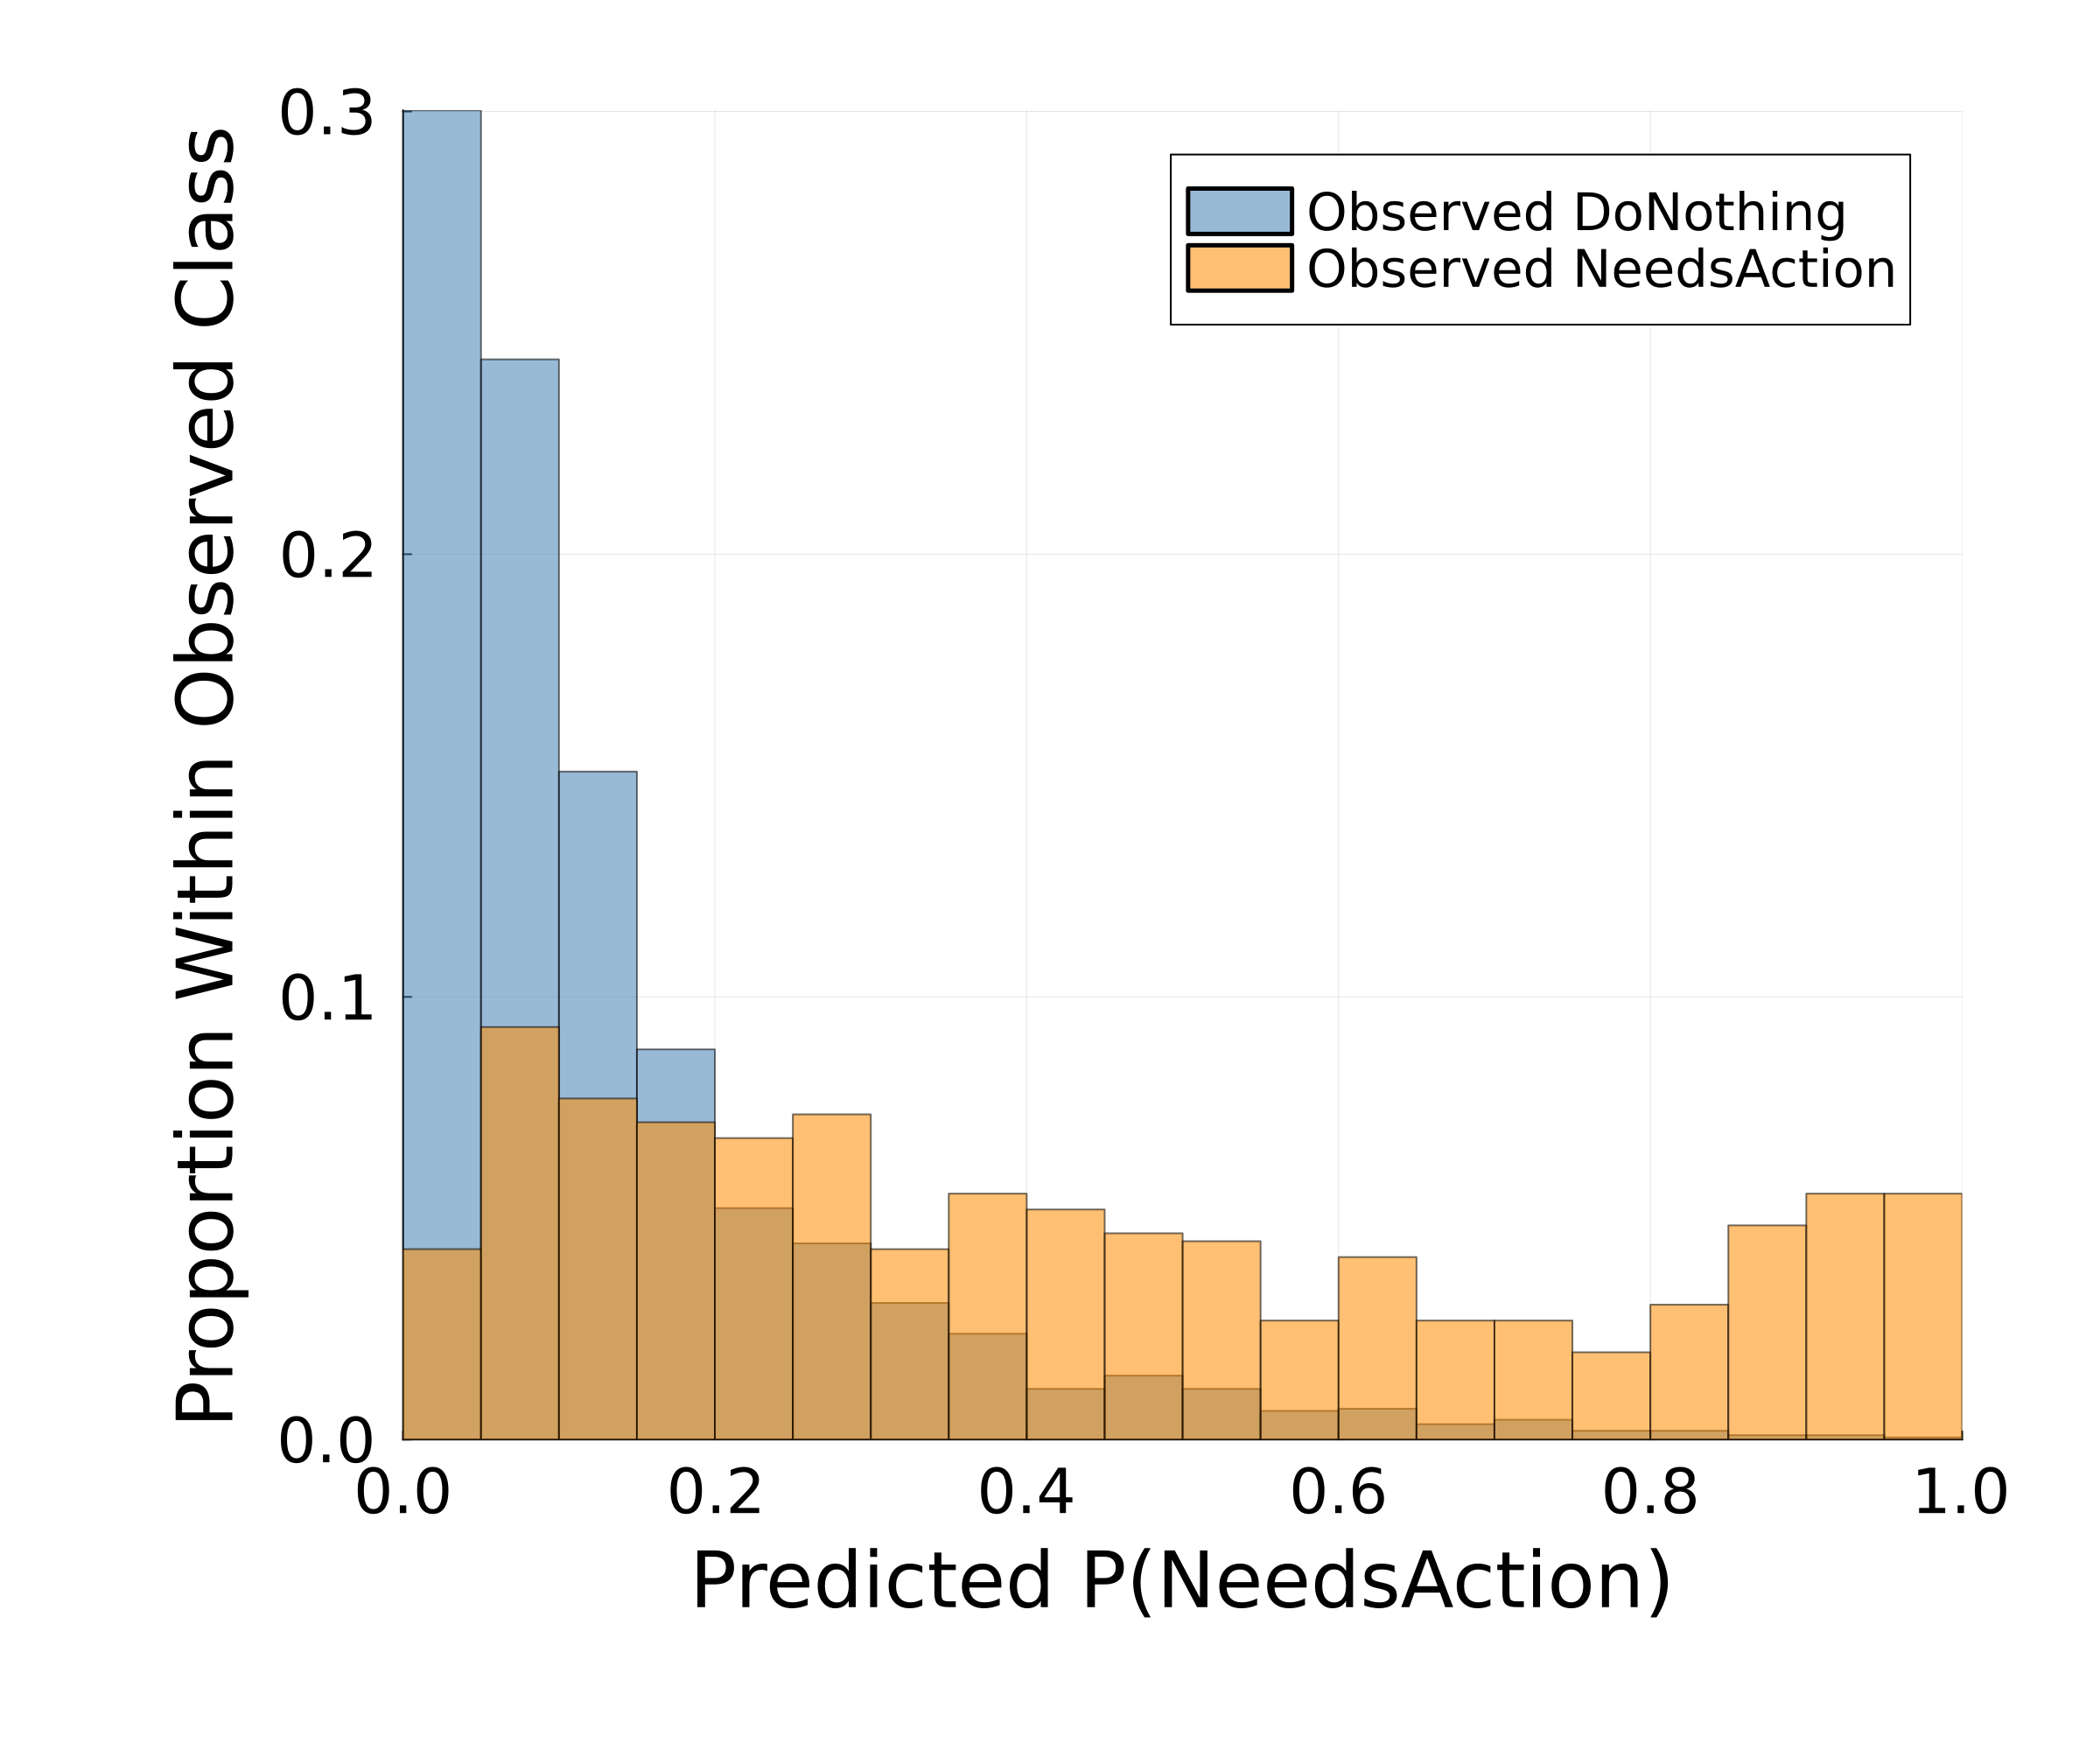
\includegraphics[width=.8\linewidth]{ANN_Probabilities_By_Region.png}
\caption{Predicted Probability by Observed Region}
\label{fig:ann_probs_by_region}
\end{figure}

Binned mean predicted NeedsAction probabilities were compared with the observed NeedsAction frequency within each bin (Figure~\ref{fig:ann_prediction_reliability}). Little deviation was reported between predicted probabilities and observed frequencies, indicating that despite the lack of clear distinction between DoNothing and NeedsAction, the frequencies of detection are consistent with the data.

\begin{figure}
\centering
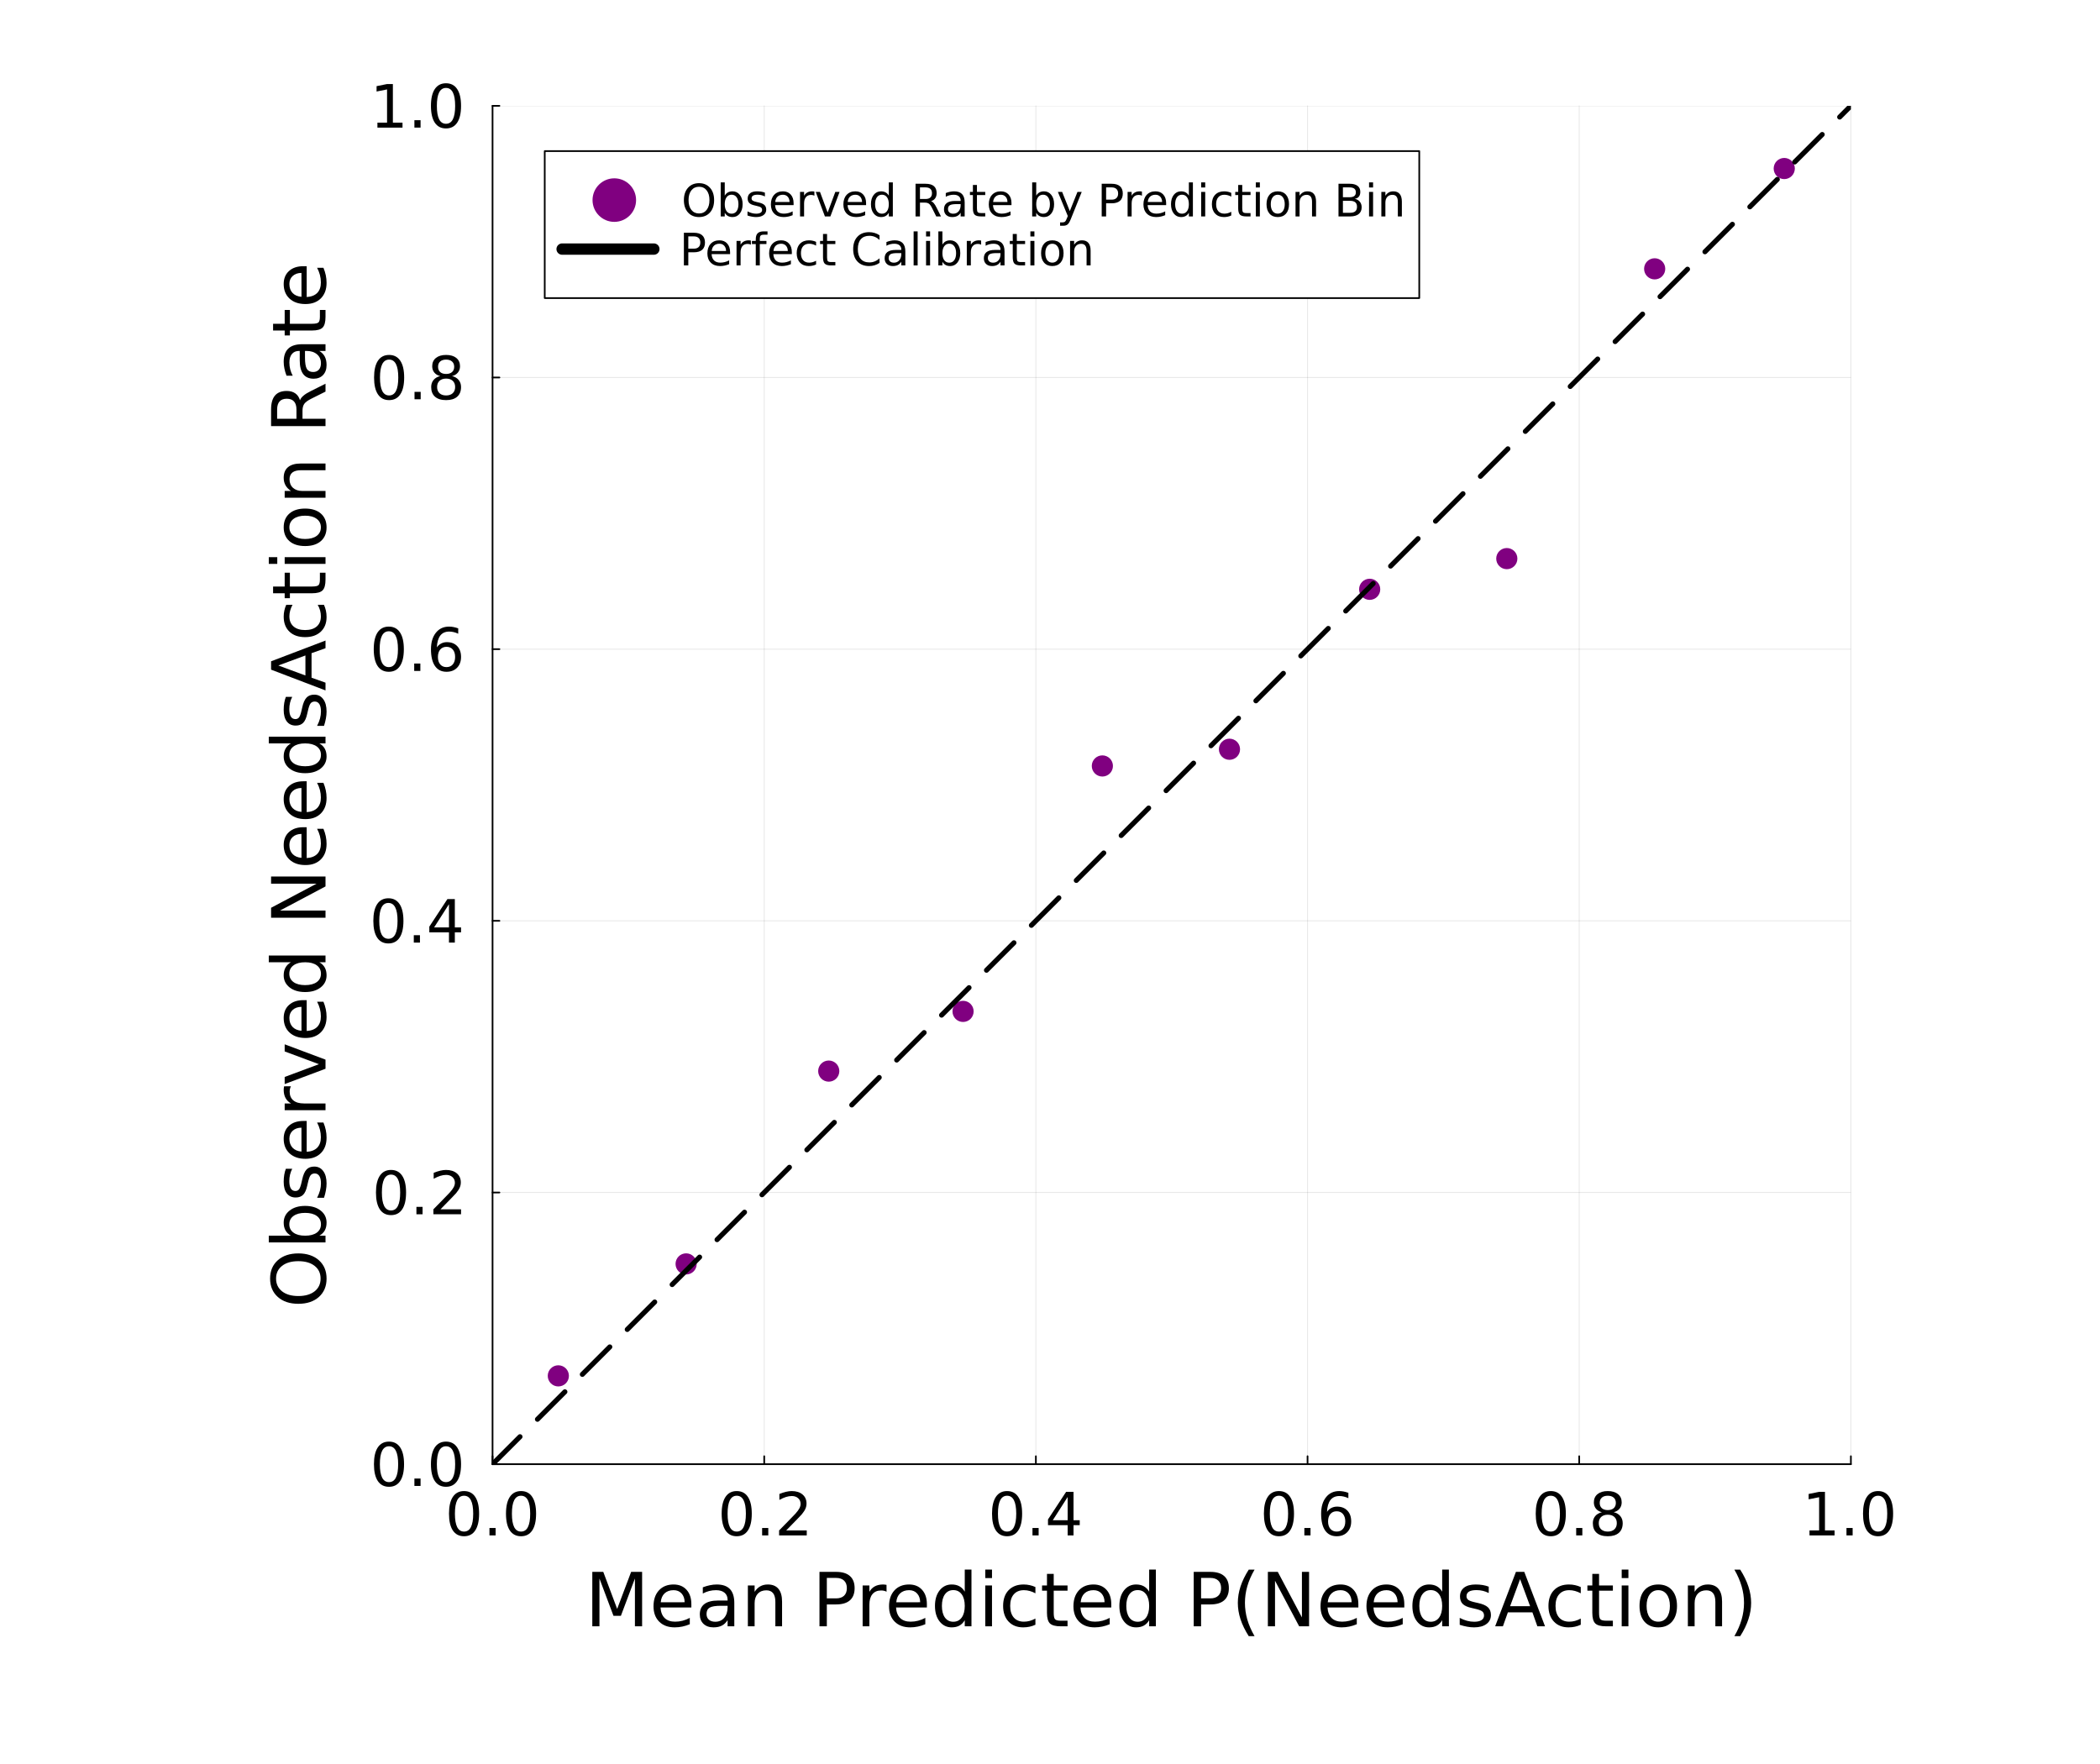
\includegraphics[width=.8\linewidth]{ANN_Prediction_Reliabilty.png}
\caption{Calibration of Predicted Probabilities}
\label{fig:ann_prediction_reliability}
\end{figure}

\FloatBarrier

\section{Discussion}

This study seeks to improve the quality of a VOI model for building boiler condition ratings by using historical assessment data to build a predictive model that accounts for previous sustainment trends by classifying boilers as "Do Nothing" or "Repair." (Refer to the Introduction for a more in-depth description of Grussing's proposed implementation of using VOI to optimize condition assessment planning \cite{grussing2018optimized}). Toward these objectives, an exploratory analysis including data visualization, correlation analysis, and principal component analysis was completed prior to the construction of three types of predictive models (logistic regression, decision tree, and ANN).

The ANN model had the best performance as measured by log-loss, although the three models had similar performance, as shown in Table~\ref{tab:model_comparison}. The logistic regression, decision tree, and ANN models had testing log loss values of 0.438, 0.416, and 0.399, respectively. In addition to the lowest held-out test log loss, the ANN also had the highest accuracy and precision at the $P(\mathrm{NeedsAction}) = 0.50$ cutoff (See Table \ref{tab:model_comparison}). The logistic regression model produced higher recall at this cutoff, but with lower precision. As described, the difference in the quality of predicted probabilities across all models was fairly small, and considering they were developed independently, this provides reasonable confidence that the models are approaching the performance potential given the available data. Additionally, although the ANN model was a far from perfect predictor of boiler maintenance classification, it still provides a practical improvement over the prevalence only approach (which had a baseline log loss of 0.524), suggesting that this study achieves the stated objective of improving the quality of the VOI model. The ANN is also an improvement upon sole reliance on the Weibull degradation model (refer to Equation 1 in the Introduction), which was not a particularly strong predictor of a boiler's actual Score, as demonstrated by the Spearman correlation coefficient of 0.50 between the two variables (refer to the Pairwise Correlation Analysis section for further details).

\begin{table}[htbp]
    \centering
    \caption{Comparison of model performance with $P(\mathrm{NeedsAction}) = 0.50$ cutoff.}
    \label{tab:model_comparison}
    \begin{tabular}{lrrrr}
        \toprule
        Model & Test Log Loss & Accuracy (\%) & Precision (\%) & Recall (\%) \\
        \midrule
        Logistic Regression & 0.438335 & 81.10 & 24.87 & 68.14 \\
        Decision Tree       & 0.413995 & 82.62 & 69.05 & 36.38 \\
        ANN                 & 0.388509 & 83.36 & 72.66 & 37.63 \\
        \bottomrule
    \end{tabular}

    \vspace{0.5em}
    \parbox{0.9\linewidth}{\footnotesize
    \textit{Note.} Log loss evaluates the quality of predicted probabilities and does not require a classification cutoff. Accuracy, precision, and recall are dependent on the selected $P(\mathrm{NeedsAction})$ cutoff and measures can change if the threshold is adjusted.}
\end{table}

Further work beyond the scope of this project may include a formal quantification of the VOI associated with the developed ANN model as a decision-making tool. Also, additional ANN configurations or types of models could be tested in an effort to improve overall model performance, although the similarity in performance of the developed models suggests that further gains may be incremental. Finally, the boilers MEC constitutes only a small subset of the observations in the full SMS BUILDER dataset, so the approaches outlined in this study may be applied to additional building components in the real estate portfolio.

\FloatBarrier

\label{section:references}
\bibliography{references}
\end{document}
